% !TEX TS-program = xelatex
% !TEX encoding = UTF-8 Unicode

% -----------------
% START OF PREAMBLE
% -----------------
\documentclass[11pt,a4paper,headinclude=false,footinclude=false]{scrreprt}
\usepackage[a4paper,top=2cm,bottom=2cm,left=3cm,right=3cm]{geometry}

% Commands
\newcommand{\HRule}{\rule{\linewidth}{0.5mm}}


% Packages
\usepackage{fontspec}
\usepackage{eurosym}
\usepackage{amssymb}
\usepackage{mathtools}
\usepackage{upquote}
\usepackage{microtype}
%\usepackage{polyglossia}
\usepackage{longtable,booktabs}
\usepackage{graphicx}
\usepackage{grffile}
\usepackage{ulem}[normalem]
\usepackage{cite}
\usepackage{hyperref}[setpagesize=false,
            unicode=false,
            colorlinks=true,
            urlcolor=blue,
	    linkcolor=black]
\usepackage{float}
\usepackage{tabu}
\usepackage{gensymb}
\usepackage{listings}


% Polyglossia settings
%\setmainlanguage{english} % or danish
%\addto\captionsenglish{%
%  \renewcommand{\contentsname}{Table of Contents}
%}


% Required for syntax highlighting



% Don't let images overflow the page
% Can still explicit set width/height/options for an image
\makeatletter
\def\maxwidth{\ifdim\Gin@nat@width>\linewidth\linewidth\else\Gin@nat@width\fi}
\def\maxheight{\ifdim\Gin@nat@height>\textheight\textheight\else\Gin@nat@height\fi}
\makeatother
\setkeys{Gin}{width=\maxwidth,height=\maxheight,keepaspectratio}


% Make links footnotes instead of hotlinks
\renewcommand{\href}[2]{#2\footnote{\url{#1}}}


% Avoid problems with \sout in headers with hyperref:
\pdfstringdefDisableCommands{\renewcommand{\sout}{}}


% No paragraph indentation
% and set space between paragraphs
\setlength{\parindent}{0pt}
\setlength{\parskip}{1em}
\setlength{\emergencystretch}{3em} % Prevent overfull lines
\renewcommand{\baselinestretch}{1.0}
\pagestyle{plain}
\pagenumbering{arabic}

% -----------------
%  END OF PREAMBLE
% -----------------
\begin{document}


\begin{titlepage}
  \begin{center}

    \textsc{\LARGE Dublin City University}\\[1.5cm]
    \textsc{\Large Electronic and Computer Engineering}\\[0.5cm]

    \HRule\\[0.4cm]
    {\huge \bfseries Streaming Audio Server with Listener-Tracking Embedded Clients\\[0.4cm]}
    \HRule\\[1.5cm]

    \begin{figure}[H]
	
\includegraphics{images/Dcu-logo.png}
	\centering
    \end{figure}

    \emph{Authors}\\[0.1cm]
    \noindent\makebox[\textwidth]{%
      \begin{tabular}{lr}%
        Michael Lenehan & \texttt{michael.lenehan4@mail.dcu.ie}\\
    \end{tabular}}\\[0.1cm]

    \emph{Supervisor}
    \noindent\makebox[\textwidth]{%
      \begin{tabular}{lr}%
        Martin Collier & \texttt{martin.collier@mail.dcu.ie}\\
    \end{tabular}}\\[1cm]

    \vfill

    % Bottom of the page
    % Probably replaced with date of deadline
      {\large{08/04/2019}}

  \end{center}
\end{titlepage}


% Chapter: 0, section: 1, subsection: 2 etc
\setcounter{secnumdepth}{1}
\setcounter{tocdepth}{1}
\tableofcontents
\listoftables
\listoffigures
%\end{document}
\chapter{Acknowledgmenets}\label{acknowledgmenets}

I would like to thank my project supervisor, Dr.~Martin Collier. He
provided guidance and assistance with all aspects of this project, and
his knowledge and insight on the topic were invaluable. I would also
like to thank Dr.~Gabriel-Miro Muntean, who acted as the second assessor
for this project. His insight into testing practices, which gave greater
clarity to the overall project results.

\begingroup
\renewcommand{\cleardoublepage}{} \renewcommand{\clearpage}{}

\chapter{Declaration}\label{declaration}

\endgroup

I declare that this material, which I now submit for assessment, is
entirely my own work and has not been taken from the work of others,
save and to the extent that such work has been cited and acknowledged
within the text of my work. I understand that plagiarism, collusion, and
copying are grave and serious offences in the university and accept the
penalties that would be imposed should I engage in plagiarism, collusion
or copying. I have read and understood the Assignment Regulations set
out in the module documentation. I have identified and included the
source of all facts, ideas, opinions, and viewpoints of others in the
assignment references. Direct quotations from books, journal articles,
internet sources, module text, or any other source whatsoever are
acknowledged and the source cited are identified in the assignment
references. This assignment, or any part of it, has not been previously
submitted by me or any other person for assessment on this or any other
course of study.

I have read and understood the DCU Academic Integrity and Plagiarism at
https://www4.dcu.ie/sites/default/files/policy/1\%20-\%20integrity\_and\_plagiarism\hspace{0pt}\_ovpaa\_v3.pdf
and IEEE referencing guidelines found at
https://loop.dcu.ie/mod/url\hspace{0pt}/view.php?id=448779.

Name: \underline{Michael Lenehan} Date: \underline{08/04/2019}

\chapter{Abstract}\label{abstract}

Open-Source audio server softwares are numerous. The most popular
available options for embedded linux devices are intended for use as
``headless'' audio devices, controlled over the network, and outputting
their audio locally. With a large number of subscription based audio
streaming services available, such as Spotify, Tidal, and Google Play
Music, there is an increasing need for an option to stream a users own
music, from a central storage device, to their client device of choice.

The addition of listener tracking allows a user to play audio through
multiple speakers as they traverse a space, such as their home, without
needing to play music through all available speakers, or without turning
device volumes up or down.

\chapter{Introduction}\label{introduction}

There are many options for open-source audio streaming available to
users. A number of configurations of the available open-source audio
streaming hardware and software allow for end-users to play locally
stored audio on a so-called ``Headless'' system, whereby the server
software is controlled remotely by the user.

In recent years, a movement away from locally stored audio solutions has
taken place. Subscription based audio streaming services such as Spotify
exist to allow users access audio which they have no access to physical
copies of. While this trend exists, an optimal server software solution
would serve both locally stored, and streaming audio options to
listeners.

This project explores the idea of implementing a streaming server which
allows users access a stored collection of audio, from any connected
device, and to stream this audio to the nearest available client device.
A solution must offer an accessible user experience, and importantly
provide good quality playback, achieved through the combination of
chosen software and hardware.

\chapter{Background Literature
Survey}\label{background-literature-survey}

\section{Hardware Requirements}\label{hardware-requirements}

\subsection{Embedded Linux Devices}\label{embedded-linux-devices}

There are a number of Linux based embedded systems which may be
configured to act as an audio streaming server with the appropriate
software. Commonly used systems include the Raspberry Pi 3 Model B+,
BeagleBone Black, and ASUS Tinker Board. There are differences between
these development platforms which allow them more or less suitability
for the purposes of this project.

The BeagleBone Black (BBB) is a low cost platform, with compatibility
for many Linux distributions. The device has on board flash memory,
Ethernet and HDMI outputs. There is also on board \(I^2S\) support,
allowing for hardware Digital to Analog Converters (DACs) to be
connected. The BBB has 512MB of DDR3 RAM, and a 1GHz ARM processor on
board\cite{BBB18}.

\begin{figure}[H]
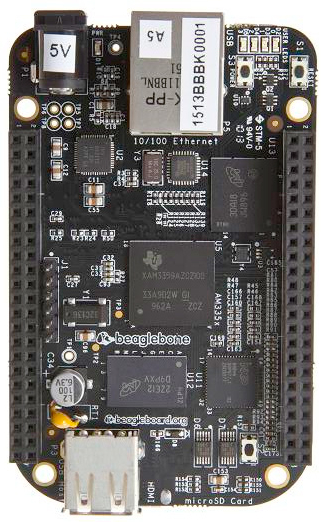
\includegraphics{BackgroundLitSurvey/BBB.jpg}
\centering
\caption{BeagleBone Black\cite{BBB18}}
\label{BBBFig}
\end{figure}

The ASUS Tinker Board is a small form-factor Single Board Computer
(SBC). The computer has Gigabit Ethernet, HDMI output, multiple IO,
including 40 GPIO pins and 4 USB ports. The 1.8GHz ARM based CPU
provides high performance when coupled with the 600MHz GPU and 2GB of
dual-channel DDR3 RAM. This SBC also supports the \(I^2S\) audio
protocol\cite{Tinker18}.

\begin{figure}[H]
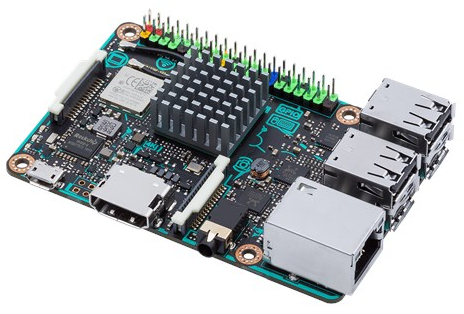
\includegraphics{BackgroundLitSurvey/AsusTB.jpeg}
\centering
\caption{Asus TinkerBoard}\cite{Tinker18}
\label{AsusTBFig}
\end{figure}

The Raspberry Pi 3 Model B+ is one of the most commonly used embedded
Linux development platforms. The device has a 1.4GHz ARM processor, 1GB
of DDR2 RAM, Gigabit Ethernet, Bluetooth Low Energy, and multiple IO
ports. Again, this board supports the \(I^2S\) protocol, with outputs on
its GPIO\cite{RPI18}.

\begin{figure}[H]
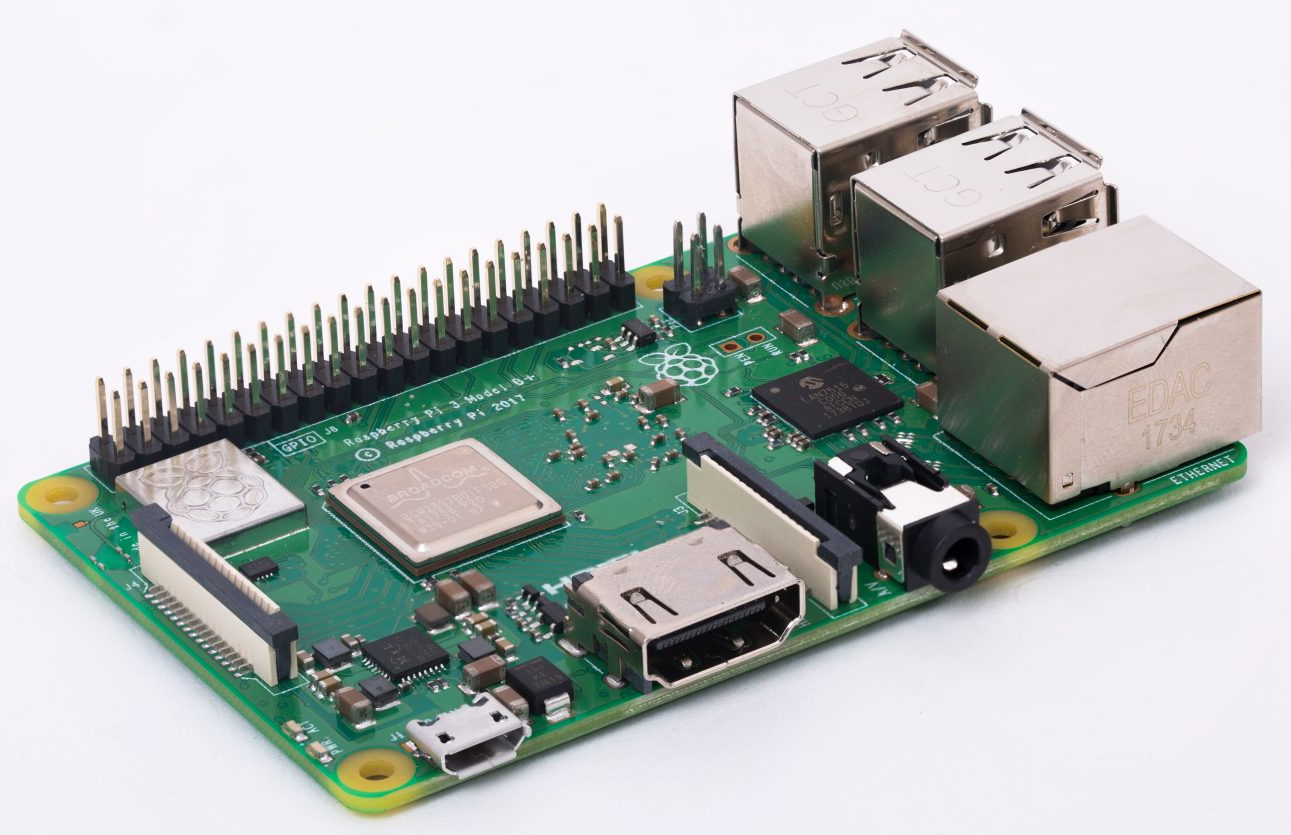
\includegraphics{BackgroundLitSurvey/Rpi.jpg}
\centering
\caption{Raspberry Pi 3 Model B+\cite{RPI18}}
\label{RPiFig}
\end{figure}

Each of the aforementioned options offers different levels of
performance at different price points. The BeagleBone Black is both the
cheapest and least powerful option. The ASUS TinkerBoard is the most
powerful and most expensive option, while the Raspberry Pi offers
comparatively high performance at a mid price. The benefits and costs of
these Single Board Computers must be compared in order to choose that
which is most appropriate for the application of serving and streaming
audio.

For the purposes of this project, the Raspberry Pi Model 3 B+ was
chosen. This platform has a large user base, and an active online
community, allowing for a more user friendly experience, especially with
regards to aspects such as initial setup and software installation. The
Raspberry Pi also has a large number of available add-on boards,
commonly referred to as ``Hats'' or ``Bonnets''. These boards may be
used to give additional functionality to the Raspberry Pi, with boards
available for purposes such as adding display capabilities, numerous
sensors, and, as is applicable to this project, audio DAC and
amplifiers.

\subsection{Audio DAC}\label{audio-dac}

As previously mentioned, there are a number of amplifier and DAC add-on
options for the Raspberry Pi 3 Model B+. Some of the most popular
options available are from HiFiBerry, including their HiFiBerry Dac+
Pro. This board offers RCA output, with dual-domain low-jitter
clocks\cite{HiFiBerry}.

The option chosen was the Adafruit I2S Audio Bonnet for Raspberry Pi.
This DAC also utilises the \(I^2S\) audio protocol, through the UDA1334A
stereo DAC. The board outputs audio via a standard 3.5mm audio jack,
with the option of soldering RCA jacks to the PCB.

\begin{figure}[H]
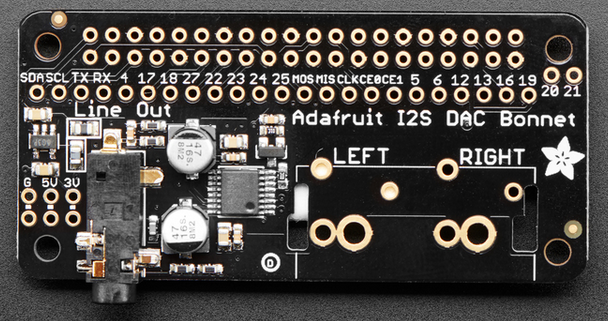
\includegraphics{BackgroundLitSurvey/adafruitdac.png}
\centering
\caption{Adafruit I2S Audio Bonnet \cite{adafruit}}
\label{AdaFig}
\end{figure}

\section{Open Source Software}\label{open-source-software}

A number of software solutions exist for streaming audio from low
powered hardware. Options such as MPD - the Music Player Daemon -,
Mopidy, and Volumio, allow for users to play music on the system. These
options are typically used to implement headless audio player setups,
with the user sending messages over the network to control the player.

While these options provide much of the basic required functionality,
they are not a suitable solution for the project. The required
functionality from the software will be to stream media from the server
system to the client system. This functionality exists in these
open-source software options, but requires modifications to be made to
configuration files in order to be implemented.

Audio software PulseAudio may also be utilised, as it is often found on
Linux based systems. PulseAudio is a sound server which routes audio
from the running application to the selected output device. On Linux
systems, this is used to send audio output to the system speakers, or
connected USB devices. However, the functionality exists to pass the
output audio over the network to a specified address\cite{Pulse14}.

\subsection{MPD}\label{mpd}

MPD is a server-side audio application, available on Debian based Linux
platforms, such as Raspbian, via the standard ``apt'' package manager
repositories. Via the available configuration files, parameters such as
the music directory, audio output device, audio encoder and decoder
plugins, and audio format settings may be set. MPD allows for playback
of a number of audio formats, including WAV, FLAC, and MP3, and supports
both FIFO, and HTTPD streaming\cite{MPD18}.

\subsection{Mopidy}\label{mopidy}

Mopidy is a server-side audio application, written in python, which
extends the functionality of MPD. It is availbale on Debian based Linux
platforms, such as Raspbian, via the standard ``apt'' package manager
respositories. In it's default configuration, Mopidy acts as a local
media server, based on MPD. The advantage of Mopidy however, lies in
it's extensibility via available ``Extensions''. These extensions
include Spotify connectivity, allowing users not only access to locally
stored audio files, but also to streaming audio.

\subsection{Volumio}\label{volumio}

Volumio is a stand alone Linux based operating system, or
``distribution'', which has been designed specifically for audio
playback\cite{Volumio18}. It is designed to be used on low powered
computers, such as the Raspberry Pi. Playback is accessible via a web
application user interface. The playback functionality of Volumio is
controlled by an MPD server.

\subsection{Snapcast}\label{snapcast}

Snapcast is a time synchronized client-server audio player. Snapcast
reads audio data from the server device, and, utilising the TCP
protocol, sends the data to all connected network client devices. Using
the aforementioned audio playback softwares, audio data can be passed to
a file, which Snapcast may then read from. Synchronicity is achieved by
passing the server's time to all clients, allowing their received data
buffers to be played back at the appropriate timing.

\section{Listener Tracking}\label{listener-tracking}

Another aspect of the project is the listener tracking and audio
routing. There are multiple protocols which may be used in order to
determine location of a mobile device. Bluetooth ``Beacons'' or Access
Points are used, sending a packet to the device, the signal strength may
be used to calculation and approximate distance\cite{Park15}. Using
filtering techniques, distances may be calculated, using Bluetooth, to
an accuracy of approximately 1.8 meters\cite{Park15}.

Location using WiFi may provide greater accuracy, however requires
specialised hardware\cite{Gjengset14}. The 802.11AC WiFi standard allows
for the use of Beamforming, in which multiple antennas transmit at once,
allowing for the targeted transmission of data\cite{Heejung14}. Using
Angle-of-Arrival (AoA), and Time-of-Flight (ToF), and Multiple Signal
Classification (MUSIC) algorithms, the distance and direction from the
Access Point may be determined \cite{Afaz18}. The operations which must
be performed are complex, and dependent on the hardware being used. As
such, less complex solutions, such as RSSI, may be implemented, however
there is also a reduction in accuracy.

\subsection{Bluetooth Beacons}\label{bluetooth-beacons}

A number of Bluetooth Beacon Specifications are currently accessible for
use on embedded Linux platforms. These specifications include
AltBeacon\cite{altbeacon}, from Radius Networks, and
Eddystone\cite{eddystone} from Google Beacon Platform. These
specifications allow for ranging requests, which provide the requesting
device with a distance estimate, based on the received signal strength
indication (RSSI) from beacon device to the user device.

\subsection{802.11MC WiFi}\label{mc-wifi}

The 802.11MC WiFi protocol provides location determination
functionality, using Round Trip Time (RTT). This protocol, if
implemented on the embedded Linux platforms, would allow for ranging
requests to be performed from Android devices on API level 28 (Android 9
``Pie'')\cite{droidRTT}.

\chapter{Concepts, Modelling, and
Design}\label{concepts-modelling-and-design}

There are two main design aspects to this project, firstly the audio
streaming server, with multiple connected devices, and secondly, the
listener tracking. Outlined are the proposed solutions to each of these
aspects, along with any complications or limitations faced.

\section{Audio Streaming}\label{audio-streaming}

The proposed design solution for the implementation of the audio
streaming system utilizes three Raspberry Pi 3 Model B+, each with a DAC
for outputting high quality audio. The chosen audio server software runs
on one device, alongside the streaming server, with the streaming
clients running on the other devices.

Figure \ref{floorplan} shows the placement of the client and server
devices, with the server being the lower of the devices on the
downstairs portion of the floor plan. This device is connected to the
network router/access point. Each of the client devices is connected to
the network via Wi-Fi.

\begin{figure}[H]
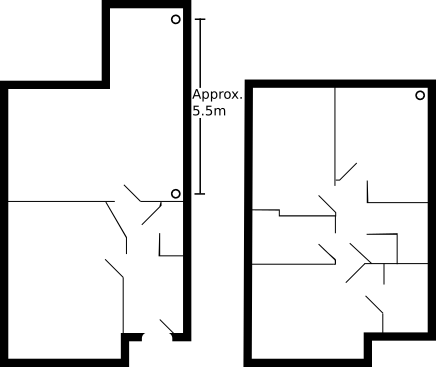
\includegraphics{ConceptsModellingDesign/floorplan.png}
\centering
\caption{Floor Plan with Downstairs (Left), Upstairs (Right), and Raspberry Pi
Locations (Represented by 'O's)}
\label{floorplan}
\end{figure}

Utilising Snapcast, multiple client devices may be connected to a
central server device, with audio playback controlled from this server
device, and transmit across the network for synchronous playback on the
client devices.

\section{Listener Tracking}\label{listener-tracking-1}

Listener tracking is implemented using a combination of Bluetooth Low
Energy Beacons, and an accompanying Android application. The BLE Beacons
must be available to be scanned from the Android application, which, in
turn, must control the volume of the audio client devices,

\subsection{Beacons}\label{beacons}

The AltBeacon BLE Beacon protocol is used for proximity data. The audio
client devices are configured using modified ``BlueZ'' example
code\cite{RPIAltBeacon}. AltBeacon is an open-source implementation of
Apple's iBeacon standard. The AltBeacon device constantly transmits
data, which is intended to be read by the Android application for the
purpose of ranging.

While there is an ``Android Beacon Library'', which allows for ranging
of Google's Eddystone Beacons\cite{beaconlibrary}, this library is not
available in Flutter, which negates the cross-platform compatibility
advantage held by Flutter applications. This is discussed further in the
following section.

The AltBeacon protocol has a data structure which has a number of
significant bytes. Bytes 7 and 8 must be set to ``0xBEAC'', which
represents the AltBeacon advertisement code\cite{altbeaconprotocol}.
Bytes 9-29 are reserved for the unique beacon identifier. In order to
correctly calibrate the AltBeacon, the average RSSI value at a distance
of 1 meter from the beacon device must be measured, and this value
placed in byte 29.

\subsection{Android Application}\label{android-application}

The proposed Android application, built using Google's ``Flutter''
framework, connects to the audio server, allowing for the control of
volume parameters. This is achieved via the transmission of JSON encoded
messages, as defined in the Snapcast JSON RPC API\cite{snaprpc}, via a
TCP socket connection from the application to the server device, on port
1705. Given an audio client device ID, which may be parsed from a server
response message, the client devices volume can be adjusted, or muted
from within the application. In order to create a JSON message in Dart,
the language used by Flutter, a number of classes and constructors are
required. The following is the Snapcast command for adjusting the volume
of a connected client device.

\lstset{
    caption=Example Snapcast "Client.SetVolume" Request,
    basicstyle=\footnotesize, frame=tb,
    xleftmargin=.2\textwidth, xrightmargin=.2\textwidth
}

\begin{lstlisting}[language=Java]
{"id":8,
"jsonrpc":"2.0",
"method":"Client.SetVolume",
"params":
    {"id":"00:21:6a:7d:74:fc",
    "volume":{"muted":false,"percent":74}
    }
}
\end{lstlisting}

As both the ``params'' and ``volume'' fields have multiple arguments,
they each require separate constructors, as follows:

\lstset{
    caption=Dart JSON "volume" Field Constructor,
    basicstyle=\footnotesize, frame=tb,
    xleftmargin=.2\textwidth, xrightmargin=.2\textwidth
}

\begin{lstlisting}[language=Java]
JSONVolume(bool mute, int percent){
    this.volume["muted"] = mute;
    this.volume["percent"] = percent;
}
\end{lstlisting}

\lstset{
    caption=Dart JSON "params" Field Constructor,
    basicstyle=\footnotesize, frame=tb,
    xleftmargin=.2\textwidth, xrightmargin=.2\textwidth
}

\begin{lstlisting}[language=Java]
JSONParams(String id, bool mute, int percent){
    this.params["id"] = id;
    this.params["volume"] = JSONVolume(mute,
    percent).volume;
}
\end{lstlisting}

Finally, the Dart equivalent of the JSON message can be constructed:

\lstset{
    caption=Dart JSON Client.SetVolume Constructor,
    basicstyle=\footnotesize, frame=tb,
    xleftmargin=.2\textwidth, xrightmargin=.2\textwidth
}

\begin{lstlisting}[language=Java]
ClientVolume(String id, bool mute, int percent){
    this.jsonMessage["id"] = 8;
    this.jsonMessage["jsonrpc"] = "2.0";
    this.jsonMessage["method"] = "Client.SetVolume";
    this.jsonMessage["params"] = JSONParams(id, mute,
    percent).params;
    this.messageString = json.encode(this.jsonMessage)
    + "\r\n";   // '\r\n' required for newline delimited
            // JSON messages
}
\end{lstlisting}

The encoded message can be transmit to the server using the
``Socket.connect(IP, Port)'', and ``Socket.write(String)'' methods. An
issue arose however in receiving the JSON response from the Snapcast
server, with notification responses being received when audio playback
was started or stopped, but no responses being received to the
``Server.GetStatus'', or ``Client.SetVolume'' requests. This meant that
client ID's could not be parsed from the server response, and, as such,
client ID's were required to be hard-coded.

The BLE Beacon ranging is implemented by utilising the Flutter
``beacons'' plugin, which supports monitoring, and ranging of both
iBeacon and AltBeacon Bluetooth Beacons\cite{flutterBeacons}. This
plugin's GitHub repository gives an example application, which, when
passed a Beacon ID performs a ranging request, printing the RSSI value
to the screen. Also provided are methods for ranging while the
application is in the background.

\lstset{
    caption=Flutter Beacons Generic Beacon Ranging,
    basicstyle=\footnotesize, frame=tb,
    xleftmargin=.2\textwidth, xrightmargin=.2\textwidth
}

\begin{lstlisting}[language=Java]
Beacons.ranging(region: BeaconRegion(
    identifier: 'test',
        ids: ['id1', 'id2', 'id3'],
      ),
      inBackground: true,
      ).listen((result) {
            final Beacon beacon = result.beacons.first;
      });
\end{lstlisting}

When combined with the volume control code, the intended implementation
is to increase volume as the listener moves closer to the client device,
and decrease the volume on the device being moved away from. This
implementation was not completed due to issues faced in Dart
development, with packages inconsistently loading correctly. This could
be due to the relative infancy of the Flutter framework, or due to an
inexperience in developing using Flutter and Dart. The advantages of
using Flutter however, are that applications, using standard packages,
and not platform specific code, may be executed on both Android and iOS
devices, for example, the JSON volume control code could be executed on
an iOS device, if available.

\section{Extensibility}\label{extensibility}

An ideal solution to the system proposed in this project would provide
extensibility, both in the number of clients, and in teh number of
concurrent users. With the implementation of Snapcast, any number of
client devices may be used, so long as the network can handle the number
of connections. Many router/access points combinations have a limit on
the nnumber of Wi-Fi devices which can be connected to the network at
once, with the Sky Q Hub used having a maximum number of 64 connected
devices\cite{SkyQ}.

As devices are added, the accuracy of the BLE beacons could act as an
obstruction to extending the number of devices. Differences in accuracy
between closely placed beacons could result in the scanning application
choosing to route audio to the incorrect client device. However, as
Snapcast can group client devices, and modify group volumes rather than
individual volumes, client devices placed in too close of a proximity
for accureate differentiation could be grouped, with one device in a
group acting as a BLE beacon.

Within the context of a home audio setup, it could be desirable to have
multiple users have separate access to audio playback, from different
client, at the same time. MPD and Mopidy can both be configure to run in
multiple instances on the same device, with different ports. From these
multiple audio server software instances, audio can be fed to Snapcast,
which has the ability to be configured with multiple streams, from
multiple inputs, which can be assigned by the useri\cite{snapcastZones}.

\chapter{Experimental Equipment and
Procedures}\label{experimental-equipment-and-procedures}

\section{Experimental Equipment
Requirements}\label{experimental-equipment-requirements}

The following hardware equipment is required for testing of both the
audio server software and the listener tracking implementations:

\begin{table}[H]
\centering
    \begin{tabular}{||c|c||}
    \hline
    \multicolumn{2}{|c|}{\textbf{Experimental Equipment}} \\
    \hline\hline
    \textbf{Description} & \textbf{Quantity} \\
    \hline\hline
    Raspberry Pi 3 Model B+ & 3 \\
    \hline
    T5989DV - AC/DC Power Supply, 1 Output, 13 W, 5.1 V, 2.4 A & 3 \\
    \hline
    Adafruit I2S Audio Bonnet for Raspberry Pi - UDA1334A & 3 \\
    \hline
    SanDisk SDSDQAF3-008G-I & 3 \\
    \hline
    Audio Amplifier/Speaker Device (with Line In) & 3 \\
    \hline
    \end{tabular}
    \caption{Required Experimental Equipment}
    \label{ExperimentalEquip}
\end{table}

\subsection{Audio Server Software Equipment
Requirements}\label{audio-server-software-equipment-requirements}

In order to follow the testing steps outlined below in Section
\ref{servertesting}, three Raspberry Pi Model 3 B+ are required, along
with three T5989DC AC/DC Power Supplies, three SanDisk Industrial 8GB
Class 10 MicroSD cards, two Adafruit I2S Audio Bonnets, and two audio
amplifier/speaker devices for audio output- This will allow for the
client server streaming implementation between two Rasperry Pi's, with
the third utilised for monitoring the devices used for streaming.

\subsection{Listener Tracking Equipment
Requirements}\label{listener-tracking-equipment-requirements}

In order to follow the testing steps outlined below in Section
\ref{servertesting}, three Raspberry Pi Model 3 B+ are required, along
with three T5989DC AC/DC Power Supplies, three SanDisk Industrial 8GB
Class 10 Micro SD cards, and one Android device. This will allow for the
Bluetooth AltBeacons to be implemented on the Raspberry Pi's, with the
Android device running the Bluetooth Beacon detection application.

\section{\texorpdfstring{Experimental Procedures
\label{expprocedure}}{Experimental Procedures }}\label{experimental-procedures}

\subsection{\texorpdfstring{Audio Server Software Testing Procedure
\label{servertesting}}{Audio Server Software Testing Procedure }}\label{audio-server-software-testing-procedure}

The testing steps outlined below will initiate playback of the available
audio files from the audio server. Audio will be played for a total of
six hours, divided amongst the three available audio formats, wave,
FLAC, and MP3. As shown below, the three available albums are
``Hardwired To Self Destruct'' by Metallica, in wave format, ``Superfuzz
Bigmuff'' by Mudhoney in FLAC format, and ``Sonic Highways'' by Foo
Fighters in MP3.

The Music Player Client ``mpc'' is used to control playback on each of
the audio server softwares. The following mpc commands are used for
playback configuration:

\begin{itemize}
 \item "add"
 \begin{itemize}
  \item Adds the specified audio to the current playlist
 \end{itemize}
 \item "repeat"
 \begin{itemize}
  \item Toggles the repeat option, or sets this option to the input argument, i.e. on
   or off
  \end{itemize}
 \item "play"
 \begin{itemize}
  \item Begins playback of the current playlist
 \end{itemize}
 \item "stop"
 \begin{itemize}
  \item Stops playback of the current playlist
 \end{itemize}
 \item "clear"
 \begin{itemize}
  \item Clears all audio files from the current playlist
 \end{itemize}
\end{itemize}

\subsection{Testing Steps:}\label{testing-steps}

The following test procedure must be followed in order to retrieve data
for the comparison of the chosen audio server softwares.

\begin{enumerate}
  \item Using ssh, connect to the audio server device
  \begin{itemize}
    \item \$ ssh pi@<Server Pi IP>
  \end{itemize}
  \item Create a crontable on the server device to start and stop audio playback
  at a set time(s):
  \begin{itemize}
    \item \$ crontab -e
    \item Enter the following lines to the crontable
    \begin{itemize}
     \item 00 10 * * * mpc add Hardwired\_To\textendash{}Self\textendash{}Destruct\_BoxSet\_WAV/ \&\& mpc repeat on \&\& mpc play
     \item 00 12 * * * mpc stop \&\& mpc clear \&\& mpc repeat off
     \item 02 12 * * * mpc add
     mudhoney\textendash{}superfuzz\_bigmuff\textendash{}flac/ \&\& mpc repeat on \&\& mpc play
     \item 02 14 * * * mpc stop \&\& mpc clear \&\& mpc repeat off
     \item 04 14 * * * mpc add Sonic\_Highways/ \&\& mpc repeat on \&\& mpc play
     \item 04 16 * * * mpc stop \&\& mpc clear \&\& mpc repeat off
   \end{itemize}
  \end{itemize}
  \item Once testing is complete of all available audio formats, replace the audio
   server software - "MPD" - with the "Mopidy" audio server software. Repeat step
   one for the "mopidy" server software.
  \item Once testing is complete of all available audio formats, replace the audio
   server software - "Mopidy" - with the "Volumio" audio server software. Repeat
   step one for the "Volumio" server software.
  \item Record the data output from Munin, available in the browser from <Munin
  Server IP>/munin.
\end{enumerate}

For analysis, compare all applicable parameters as recorded from Munin.
The results and analysis may be seen in Section
\ref{AudioServerSoftwareResults}.

\subsection{Listener Tracking Testing
Procedure}\label{listener-tracking-testing-procedure}

The testing steps outlined below will test the ranging capabilities of
three Bluetooth Beacons, as measured using an Android Smartphone. Three
AltBeacons, running on Raspberry Pi 3 Model B+, are scanned for, with
ranging requests done at distances of 1-5 meters at one meter intervals.

Nicolas Bridoux's ``Beacon Scanner'' Android
application\cite{beaconscan} is used in order to approximate the
distance from the Android device to the AltBeacon, utilising bluetooth
RSSI to estimate this distance. The following information may be taken
from the application:

\begin{itemize}
 \item "Beacon Type"
 \begin{itemize}
  \item Returns the type of bluetooth beacon being used, e.g. iBeacon,
  Eddystone Beacon, and AltBeacon
 \end{itemize}
 \item "Beacon ID"
 \begin{itemize}
  \item The UUID for the beacon being used
 \end{itemize}
 \item "RSSI"
 \begin{itemize}
  \item The Received Signal Strength Indication from the bluetooth beacon to
  the Android device
 \end{itemize}
 \item "TX"
 \begin{itemize}
  \item The signal transmission strength from the bluetooth beacon
 \end{itemize}
\end{itemize}

\subsection{Testing Steps:}\label{testing-steps-1}

The following test procedure must be followed in order to retrieve data
for the ranging accuracy of the bluetooth beacons.

\begin{enumerate}
 \item Using ssh, connect to the bluetooth beacon device.
 \begin{itemize}
  \item \$ ssh pi@<Beacon Device IP>
 \end{itemize}
 \item Execute the AltBeacon script on the Raspberry Pi.
 \begin{itemize}
  \item \$ sudo ./altbeacon
 \end{itemize}
 \item Enable Bluetooth on the Android device.
 \item Run the Beacon Scanner application on the Android device.
 \item Place the Android device at a distance of 1m from the beacon device.
 \item Begin scanning for bluetooth devices.
 \item Record the estimated distance from the beacon device to the Android
 device.
 \item Repeat steps 5-7 for distances of 2, 3, 4, and 5 meters.
\end{enumerate}

For analysis, compare all distance measured in the Beacon Scanner
application with the actual distance. The results and analysis may be
seen in Section \ref{clienttrackresults}.

\chapter{Implementation and Testing}\label{implementation-and-testing}

\section{\texorpdfstring{Audio Server Software Implementation
\label{audioserverimplementation}}{Audio Server Software Implementation }}\label{audio-server-software-implementation}

In order to excecute the required testing of the audio server software,
the following softwares must be installed on the server device, and the
following configurations completed.

\subsection{SSH}\label{ssh}

SSH is a protocol used for end-to-end client-server secure
connections\cite{ssh}. SSH allows for remote login, and file transfers,
from a client to a server device, i.e.~from a development PC to an
embedded Linux device. SSH utilises ``keys'' for authentication, and
provides secure encryption between the client and server. Within this
project, SSH is used in order to log in to, and run commands on the
Raspberry Pi's, which do not have a graphical desktop environment.

\subsection{Munin}\label{munin}

Munin is a server performance monitoring software, which runs on an
Apache server, with the client software running on each device requiring
monitoring \cite{MuninMonitoring}. The recorded information is hosted on
a locally accessible website, at the IP address of the server device.
The output information is displayed in graphical representation, which
can be analysed.

\subsection{Cron}\label{cron}

Cron is a scheduling utility, which allows for the automation of command
execution at specified times, or set time intervals \cite{crontab}.
Using a crontable, a file for entering cron jobs, the required testing
schedule can be run on the audio server Raspberry Pi. For the purposes
of testing the audio server software while streaming audio files of
different formats, a crontable is configured to play audio in the Wave
format, followed by audio in the FLAC format, followed by audio in the
MP3 format. Each audio format is played continuously for two hours, with
a two minute space between formats.

\subsection{MPC}\label{mpc}

MPC is the ``Music Player Controller'', a software used for controlling
MPD, or MPD derived softwares \cite{mpc}. As such, it may be used to
control MPD, Mopidy, and Volumio. Within the audio server software
testing procedure, MPC is used in order to queue, play, and stop audio
playback on each of the server configurations.

\subsection{Configurations}\label{configurations}

On the MPD server device, the configuration file, found at the location
``/etc/mpd.conf'' must be modified in order to output audio to the
Snapcast server. The default ``ALSA'' output must first be deleted, and
a new ``FIFO'' output must be added as follows:

\lstset{
    caption=MPD SnapServer Configuration,
    basicstyle=\footnotesize, frame=tb,
    xleftmargin=.2\textwidth, xrightmargin=.2\textwidth
}

\begin{lstlisting}[language=bash]
audio_output {
    type    "fifo"
    name    "my pipe"
    path    "/tmp/snapfifo"
    format  "48000:16:2"
    mixer_type  "software"
}
\end{lstlisting}

On the Mopidy server device, the configuration file, found at the
location ``/etc/mopidy/mopidy.conf'' must be modified in order to output
audio to the Snapcast server. The defualt audio output must be removed,
with a new ``filesink'' output added as follows:

\lstset{
    caption=Mopidy SnapServer Configuration,
    basicstyle=\footnotesize, frame=tb,
    xleftmargin=.2\textwidth, xrightmargin=.2\textwidth
}

\begin{lstlisting}[language=bash]
[audio]
output = audioresample ! audioconvert !
audio/x-raw,rate=48000,channels=2,format=S16LE
! wavenc ! filesink location=/tmp/snapfifo
\end{lstlisting}

These audio outputs are used to feed audio to the Snapcast server, to be
send via the network to the Snapcast client devices. The MPD
configuration can also be used on the Volumio server, as Volumio
utilises MPD and it's configuration files for its audio playback.

\section{Audio Server Software
Testing}\label{audio-server-software-testing}

A number of parameters must be tested in order to determine the optimal
open-source audio server solution. Each audio server software is tested
under equal testing conditions, with the values for network usage, CPU
temperature, CPU load, and CPU frequency monitored and recorded.

Testing setup consists of three Raspberry Pi's, each running the
Raspbian Stretch Light OS, with the exception of the Volumio server test
configuration. One Raspberry Pi runs the audio server software, and the
Snapcast server software. The second Raspberry Pi runs the Snapclient
software. The final Raspberry Pi runs the Munin server software,
allowing to monitor the clients, which are running on the other two
Raspberry Pi's. Both the audio server device and the Munin server device
are connected to the network router/access point via Ethernet, with the
client device connected to the network wirelessly.

Munin returns graphs of system parameters for the system being
monitored. The graphs are divided into the categories of ``Network'',
``Processes'', ``System'', and ``Sensors''. The information contained in
these graphs must be extracted, with the maximum, minimum, and average
parameter values placed in a table for analysis.

\section{Listener Tracking
Implementation}\label{listener-tracking-implementation}

In order to execute the required testing of the listener tracking, the
following softwares must be installed, and the following configurations
completed on the beacon devices, and the Android device.

\subsection{SSH}\label{ssh-1}

As described in Section \ref{audioserverimplementation}, SSH allows for
the remote login from a client device to a server device, allowing for
commands to be run on the Raspberry Pi, sent from a client PC.

\subsection{BlueZ}\label{bluez}

BlueZ is the ``Official Linux Bluetooth protocol stack''\cite{bluez}.
BlueZ provides a number of code examples for creating bluetooth beacons,
using the AltBeacon protocol. These examples can be modified for the
creation of AltBeacons with unique ID's, and allow for the calibration
of these beacons.

\subsection{Beacon Scanner
Application}\label{beacon-scanner-application}

The Beacon Scanner android application allows for the monitoring and
ranging of bluetooth beacons from an android device\cite{beaconscan}.
Utilising Bluetooth RSSI, the application estimates the distance from
the Android device to the Bluetooth beacon. The device reports on beacon
type, ID, RSSI, and Transmission power. These parameters allow for the
identification and calibration of the beacon, along with the location
determination for the client.

\section{Listener Tracking Testing}\label{listener-tracking-testing}

In order to determine the accuracy and reliability of a Bluetooth
Beacon, specifically the AltBeacon protocol, for the purposes of
distance measurements in client tracking applications, a number of
readings must be taken, at multiple distances from the beacon. This will
show how the measured distance value changes with an increase in
physical distance from beacon to scanning device.

Testing setup consists of three Raspberry Pi's, each running the
Raspbian Stretch Light OS, with an AltBeacon with a unique ID. The
AltBeacons must be calibrated, by taking the RSSI value at 1 meter from
the beacon device. The value is added into byte 29 of the AltBeacon,
allowing for the beacon to more accurately provide ranging information.
An Android device running the ``Beacon Scanner'' application is used to
measure the RSSI value, and in turn to calculate an approximate distance
to the beacon.

The distance results obtained from the execution of the testing steps
outlined in Section \ref{expprocedure} must be utilised to create tables
of physical distance, estimated distance, and the deviation of the
estimate from the actual distance. As such, these tables may be used in
the analysis of the accuracy of bluetooth beacons in location
determination.

\chapter{Results and Analysis}\label{results-and-analysis}

The following results and analysis have been completed following testing
of the audio server softwares, and the client tracking, as described in
Section \ref{servertesting}.

\section{\texorpdfstring{Audio Server Software
\label{AudioServerSoftwareResults}}{Audio Server Software }}\label{audio-server-software}

The following tables have been extracted from the data collected from
Munin. A full list of results can be found within the Appendices Section
\ref{AppendicesAudioServerSoftwareTables}. The client and server data
has been combined under the headings of Network, System, and Sensors,
for each of the audio server software solutions.

\subsection{MPD}\label{mpd-1}

The network information for the MPD Server and SnapClient configuration
below shows there are no Ethernet errors or traffic on the Client
device, as it is connected to the network via WiFi. Conversely, on the
Server device, there are Wireless network errors, and traffic values, as
the server device is both setup on the network via WiFi and Ethernet.

\begin{table}[H]
\centering
    \begin{tabular}{||c|c|c|c|c|c|c||}
    \hline
    \multicolumn{7}{|c|}{\textbf{Network}} \\
    \hline
    \multicolumn{7}{|c|}{\textbf{Eth0 Errors (Client)}} \\
    \hline\hline
      & \multicolumn{2}{|c|}{Min} & \multicolumn{2}{|c|}{Avg} & \multicolumn{2}{|c|}{Max} \\
    \hline
     & - & + & - & + & - & + \\
    \hline
    Errors & 0.00 & 0.00 & 0.00 & 0.00 & 0.00 & 0.00 \\
    \hline
    Drops & 0.00 & 0.00 & 0.00 & 0.00 & 0.00 & 0.00 \\
    \hline
    Collisions & 0.00 & 0.00 & 0.00 & 0.00 & 0.00 & 0.00 \\
    \hline\hline
    \multicolumn{7}{|c|}{\textbf{Eth0 Errors (Server)}} \\
    \hline\hline
      & \multicolumn{2}{|c|}{Min} & \multicolumn{2}{|c|}{Avg} & \multicolumn{2}{|c|}{Max} \\
    \hline
     & - & + & - & + & - & + \\
    \hline
    Errors & 0.00 & 0.00 & 0.00 & 0.00 & 0.00 & 0.00 \\
    \hline
    Drops & 830.03m & 0.00 & 835.49m & 0.00 & 853.19m & 0.00 \\
    \hline
    Collisions & 0.00 & 0.00 & 0.00 & 0.00 & 0.00 & 0.00 \\
    \hline\hline
    \multicolumn{7}{|c|}{\textbf{Eth0 Traffic (Client)}} \\
    \hline\hline
      & \multicolumn{2}{|c|}{Min} & \multicolumn{2}{|c|}{Avg} & \multicolumn{2}{|c|}{Max} \\
    \hline
      & - & + & - & + & - & + \\
    \hline
    bps & 0.00 & 0.00 & 0.00 & 0.00 & 0.00 & 0.00 \\
    \hline\hline
    \multicolumn{7}{|c|}{\textbf{Eth0 Traffic (Server)}} \\
    \hline\hline
      & \multicolumn{2}{|c|}{Min} & \multicolumn{2}{|c|}{Avg} & \multicolumn{2}{|c|}{Max} \\
    \hline
      & - & + & - & + & - & + \\
    \hline
    bps & 1.25k & 1.31k & 23.66k & 951.47k & 29.07k & 1.27M \\
    \hline\hline
    \multicolumn{7}{|c|}{\textbf{Wlan0 Errors (Client)}} \\
    \hline\hline
      & \multicolumn{2}{|c|}{Min} & \multicolumn{2}{|c|}{Avg} & \multicolumn{2}{|c|}{Max} \\
    \hline
      & - & + & - & + & - & + \\
    \hline
    Errors  & 0.00 & 0.00 & 0.00 & 0.00 & 0.00 & 0.00 \\
    \hline
    Drops & 270.53m & 0.00 & 302.72m & 0.00 & 343.80m & 0.00 \\
    \hline
    Collisions & \multicolumn{2}{|c|}{0.00} & \multicolumn{2}{|c|}{0.00} & \multicolumn{2}{|c|}{0.00} \\
    \hline\hline
    \multicolumn{7}{|c|}{\textbf{Wlan0 Errors (Server)}} \\
    \hline\hline
      & \multicolumn{2}{|c|}{Min} & \multicolumn{2}{|c|}{Avg} & \multicolumn{2}{|c|}{Max} \\
    \hline
      & - & + & - & + & - & + \\
    \hline
    Errors  & 0.00 & 0.00 & 0.00 & 0.00 & 0.00 & 0.00 \\
    \hline
    Drops & 327.00m & 0.00 & 335.22m & 0.00 & 349.93m & 0.00 \\
    \hline
    Collisions & \multicolumn{2}{|c|}{0.00} & \multicolumn{2}{|c|}{0.00} & \multicolumn{2}{|c|}{0.00} \\
    \hline\hline
    \multicolumn{7}{|c|}{\textbf{Wlan0 Traffic (Client)}} \\
    \hline\hline
      & \multicolumn{2}{|c|}{Min} & \multicolumn{2}{|c|}{Avg} & \multicolumn{2}{|c|}{Max} \\
    \hline
      & - & + & - & + & - & + \\
    \hline
    bps  & 669.92 & 1.58k & 939.62k & 31.80k & 1.26M & 39.03k \\
    \hline\hline
    \multicolumn{7}{|c|}{\textbf{Wlan0 Traffic (Server)}} \\
    \hline\hline
      & \multicolumn{2}{|c|}{Min} & \multicolumn{2}{|c|}{Avg} & \multicolumn{2}{|c|}{Max} \\
    \hline
      & - & + & - & + & - & + \\
    \hline
    bps  & 186.42 & 17.12 & 321.71 & 22.45 & 741.32 & 39.21 \\
    \hline\hline
    \end{tabular}
    \caption{MPD Server and SnapClient Device Network Parameters}
    \label{MPDclientserverNetTab}
\end{table}

Within the Munin system measurements, it can be seen that on the Server
device, approximately 964MB of the 1GB of DDR2 RAM on the Raspberry Pi
Model 3B+ is in use on average, with average system load of 0.41, and
CPU usage of 5.89\% (idling at 92\% - Note: The Munin monitoring
software measures CPU usage percentage from 0-400\%, i.e.~usage on each
CPU core). On the Client device, approximately 327MB of the 1GB of DDR2
RAM is in use on average, with average system load of 0.13, and CPU
usage of 3.35\% (idling at 96\%)

\begin{table}[H]
\centering
    \begin{tabular}{||c|c|c|c|c|c|c||}
    \hline
    \multicolumn{7}{|c|}{\textbf{System}} \\
    \hline
    \multicolumn{7}{|c|}{\textbf{Load Average (Client)}} \\
    \hline\hline
      & \multicolumn{2}{|c|}{Min} & \multicolumn{2}{|c|}{Avg} & \multicolumn{2}{|c|}{Max} \\
    \hline
    Load & \multicolumn{2}{|c|}{0.02} & \multicolumn{2}{|c|}{0.13} & \multicolumn{2}{|c|}{0.46} \\
    \hline\hline
    \multicolumn{7}{|c|}{\textbf{Load Average (Server)}} \\
    \hline\hline
      & \multicolumn{2}{|c|}{Min} & \multicolumn{2}{|c|}{Avg} & \multicolumn{2}{|c|}{Max} \\
    \hline
    Load & \multicolumn{2}{|c|}{0.03} & \multicolumn{2}{|c|}{0.41} & \multicolumn{2}{|c|}{1.03} \\
    \hline\hline
    \multicolumn{7}{|c|}{\textbf{Memory Usage (Bytes) (Client)}} \\
    \hline\hline
      & \multicolumn{2}{|c|}{Min} & \multicolumn{2}{|c|}{Avg} & \multicolumn{2}{|c|}{Max} \\
    \hline
    Active & \multicolumn{2}{|c|}{164.04M} & \multicolumn{2}{|c|}{165.38M} & \multicolumn{2}{|c|}{167.67M} \\
    \hline
    Inactive & \multicolumn{2}{|c|}{51.14M} & \multicolumn{2}{|c|}{51.17M} & \multicolumn{2}{|c|}{51.21M} \\
    \hline
    Unused & \multicolumn{2}{|c|}{670.26M} & \multicolumn{2}{|c|}{673.18M} & \multicolumn{2}{|c|}{675.15M} \\
    \hline\hline
    \multicolumn{7}{|c|}{\textbf{Memory Usage (Bytes) (Server)}} \\
    \hline\hline
      & \multicolumn{2}{|c|}{Min} & \multicolumn{2}{|c|}{Avg} & \multicolumn{2}{|c|}{Max} \\
    \hline
    Active & \multicolumn{2}{|c|}{270.40M} & \multicolumn{2}{|c|}{408.59M} & \multicolumn{2}{|c|}{437.63M} \\
    \hline
    Inactive & \multicolumn{2}{|c|}{424.17M} & \multicolumn{2}{|c|}{541.23M} & \multicolumn{2}{|c|}{589.36M} \\
    \hline
    Unused & \multicolumn{2}{|c|}{31.03M} & \multicolumn{2}{|c|}{35.88M} & \multicolumn{2}{|c|}{43.78M} \\
    \hline\hline
    \multicolumn{7}{|c|}{\textbf{CPU Usage (\%) (Client)}} \\
    \hline\hline
      & \multicolumn{2}{|c|}{Min} & \multicolumn{2}{|c|}{Avg} & \multicolumn{2}{|c|}{Max} \\
    \hline
    System & \multicolumn{2}{|c|}{1.05} & \multicolumn{2}{|c|}{3.35} & \multicolumn{2}{|c|}{9.27} \\
    \hline
    Idle & \multicolumn{2}{|c|}{381.73} & \multicolumn{2}{|c|}{384.41} & \multicolumn{2}{|c|}{394.69} \\
    \hline\hline
    \multicolumn{7}{|c|}{\textbf{CPU Usage (\%) (Server)}} \\
    \hline\hline
      & \multicolumn{2}{|c|}{Min} & \multicolumn{2}{|c|}{Avg} & \multicolumn{2}{|c|}{Max} \\
    \hline
    System & \multicolumn{2}{|c|}{1.21} & \multicolumn{2}{|c|}{5.89} & \multicolumn{2}{|c|}{15.08} \\
    \hline
    Idle & \multicolumn{2}{|c|}{363.71} & \multicolumn{2}{|c|}{369.60} & \multicolumn{2}{|c|}{394.16} \\
    \hline\hline
    \end{tabular}
    \caption{MPD Server and SnapClient Device System Parameters}
    \label{MPDclientserverSysTab}
\end{table}

The Raspberry Pi CPU frequency and temperature were measured using a
Munin plugin. The Client device kept an average frequency of 600MHz,
with average frequency scaling of 618.10MHz on CPU core 1 and 2, and
average frequency scaling of 610.10MHz on CPU core 3 and 4. The average
temperature of the Client device is 42.66 \degree C.

The Server device had an average frequency of 656.53MHz, however at
times reached its maximum frequency of 1.4GHz. On CPU cores 1-4 the
average frequency scaling is 691.30MHz, and had an average temperature
of 56.11 \degree C.

\begin{table}[H]
\centering
    \begin{tabular}{||c|c|c|c|c|c|c||}
    \hline
    \multicolumn{7}{|c|}{\textbf{Sensors}} \\
    \hline
    \multicolumn{7}{|c|}{\textbf{CPU Frequency (MHz) (Client)}} \\
    \hline\hline
      & \multicolumn{2}{|c|}{Min} & \multicolumn{2}{|c|}{Avg} & \multicolumn{2}{|c|}{Max} \\
    \hline
    CPU & \multicolumn{2}{|c|}{600.00} & \multicolumn{2}{|c|}{600.00} & \multicolumn{2}{|c|}{600.00} \\
    \hline\hline
    \multicolumn{7}{|c|}{\textbf{CPU Frequency (MHz) (Server)}} \\
    \hline\hline
      & \multicolumn{2}{|c|}{Min} & \multicolumn{2}{|c|}{Avg} & \multicolumn{2}{|c|}{Max} \\
    \hline
    CPU & \multicolumn{2}{|c|}{600.00} & \multicolumn{2}{|c|}{656.53} & \multicolumn{2}{|c|}{1.40k} \\
    \hline\hline
    \multicolumn{7}{|c|}{\textbf{CPU Frequency Scaling (MHz) (Client)}} \\
    \hline
      & \multicolumn{2}{|c|}{Min} & \multicolumn{2}{|c|}{Avg} & \multicolumn{2}{|c|}{Max} \\
    \hline
    CPU1 & \multicolumn{2}{|c|}{613.87} & \multicolumn{2}{|c|}{618.10} & \multicolumn{2}{|c|}{620.98} \\
    \hline
    CPU2 & \multicolumn{2}{|c|}{613.92} & \multicolumn{2}{|c|}{618.10} & \multicolumn{2}{|c|}{620.97} \\
    \hline
    CPU3 & \multicolumn{2}{|c|}{613.87} & \multicolumn{2}{|c|}{610.10} & \multicolumn{2}{|c|}{620.99} \\
    \hline
    CPU4 & \multicolumn{2}{|c|}{613.92} & \multicolumn{2}{|c|}{610.10} & \multicolumn{2}{|c|}{620.98} \\
    \hline\hline
    \multicolumn{7}{|c|}{\textbf{CPU Frequency Scaling (MHz) (Server)}} \\
    \hline
      & \multicolumn{2}{|c|}{Min} & \multicolumn{2}{|c|}{Avg} & \multicolumn{2}{|c|}{Max} \\
    \hline
    CPU1 & \multicolumn{2}{|c|}{624.32} & \multicolumn{2}{|c|}{691.30} & \multicolumn{2}{|c|}{842.15} \\
    \hline
    CPU2 & \multicolumn{2}{|c|}{624.32} & \multicolumn{2}{|c|}{691.30} & \multicolumn{2}{|c|}{842.12} \\
    \hline
    CPU3 & \multicolumn{2}{|c|}{624.30} & \multicolumn{2}{|c|}{691.30} & \multicolumn{2}{|c|}{842.14} \\
    \hline
    CPU4 & \multicolumn{2}{|c|}{624.30} & \multicolumn{2}{|c|}{691.30} & \multicolumn{2}{|c|}{842.11} \\
    \hline\hline
    \multicolumn{7}{|c|}{\textbf{CPU Temperature (\degree C) (Client)}} \\
    \hline\hline
      & \multicolumn{2}{|c|}{Min} & \multicolumn{2}{|c|}{Avg} & \multicolumn{2}{|c|}{Max} \\
    \hline
    CPU & \multicolumn{2}{|c|}{41.86} & \multicolumn{2}{|c|}{42.66} & \multicolumn{2}{|c|}{44.00} \\
    \hline\hline
    \multicolumn{7}{|c|}{\textbf{CPU Temperature (\degree C) (Server)}} \\
    \hline\hline
      & \multicolumn{2}{|c|}{Min} & \multicolumn{2}{|c|}{Avg} & \multicolumn{2}{|c|}{Max} \\
    \hline
    CPU & \multicolumn{2}{|c|}{53.69} & \multicolumn{2}{|c|}{56.11} & \multicolumn{2}{|c|}{58.52} \\
    \hline\hline
    \end{tabular}
    \caption{MPD Server and SnapClient Device Sensor Parameters}
    \label{MPDclientserverSensorTab}
\end{table}

\subsection{Mopidy}\label{mopidy-1}

The network information for the Mopidy Server and SnapClient
configuration below, again, shows that there are no Ethernet errors or
traffic on the Client device, due to the network connection being
wireless. The Server device has both wireless and wired errors and
traffic.

\begin{table}[H]
\centering
    \begin{tabular}{||c|c|c|c|c|c|c||}
    \hline
    \multicolumn{7}{|c|}{\textbf{Network}} \\
    \hline
    \multicolumn{7}{|c|}{\textbf{Eth0 Errors (Client)}} \\
    \hline\hline
      & \multicolumn{2}{|c|}{Min} & \multicolumn{2}{|c|}{Avg} & \multicolumn{2}{|c|}{Max} \\
    \hline
     & - & + & - & + & - & + \\
    \hline
    Errors & 0.00 & 0.00 & 0.00 & 0.00 & 0.00 & 0.00 \\
    \hline
    Drops & 0.00 & 0.00 & 0.00 & 0.00 & 0.00 & 0.00 \\
    \hline
    Collisions & 0.00 & 0.00 & 0.00 & 0.00 & 0.00 & 0.00 \\
    \hline\hline
    \multicolumn{7}{|c|}{\textbf{Eth0 Errors (Server)}} \\
    \hline\hline
      & \multicolumn{2}{|c|}{Min} & \multicolumn{2}{|c|}{Avg} & \multicolumn{2}{|c|}{Max} \\
    \hline
     & - & + & - & + & - & + \\
    \hline
    Errors & 0.00 & 0.00 & 0.00 & 0.00 & 0.00 & 0.00 \\
    \hline
    Drops & 827.43m & 0.00 & 835.03m & 0.00 & 852.73m & 0.00 \\
    \hline
    Collisions & 0.00 & 0.00 & 0.00 & 0.00 & 0.00 & 0.00 \\
    \hline\hline
    \multicolumn{7}{|c|}{\textbf{Eth0 Traffic (Client)}} \\
    \hline\hline
      & \multicolumn{2}{|c|}{Min} & \multicolumn{2}{|c|}{Avg} & \multicolumn{2}{|c|}{Max} \\
    \hline
      & - & + & - & + & - & + \\
    \hline
    bps & 0.00 & 0.00 & 0.00 & 0.00 & 0.00 & 0.00 \\
    \hline\hline
    \multicolumn{7}{|c|}{\textbf{Eth0 Traffic (Server)}} \\
    \hline\hline
      & \multicolumn{2}{|c|}{Min} & \multicolumn{2}{|c|}{Avg} & \multicolumn{2}{|c|}{Max} \\
    \hline
      & - & + & - & + & - & + \\
    \hline
    bps & 1.23k & 1.34k & 25.65k & 961.24k & 35.72k & 1.34M \\
    \hline\hline
    \multicolumn{7}{|c|}{\textbf{Wlan0 Errors (Client)}} \\
    \hline\hline
      & \multicolumn{2}{|c|}{Min} & \multicolumn{2}{|c|}{Avg} & \multicolumn{2}{|c|}{Max} \\
    \hline
      & - & + & - & + & - & + \\
    \hline
    Errors  & 0.00 & 0.00 & 0.00 & 0.00 & 0.00 & 0.00 \\
    \hline
    Drops & 313.56m & 0.00 & 330.82m & 0.00 & 344.32m & 0.00 \\
    \hline
    Collisions & \multicolumn{2}{|c|}{0.00} & \multicolumn{2}{|c|}{0.00} & \multicolumn{2}{|c|}{0.00} \\
    \hline\hline
    \multicolumn{7}{|c|}{\textbf{Wlan0 Errors (Server)}} \\
    \hline\hline
      & \multicolumn{2}{|c|}{Min} & \multicolumn{2}{|c|}{Avg} & \multicolumn{2}{|c|}{Max} \\
    \hline
      & - & + & - & + & - & + \\
    \hline
    Errors  & 0.00 & 0.00 & 0.00 & 0.00 & 0.00 & 0.00 \\
    \hline
    Drops & 329.11m & 0.00 & 334.61m & 0.00 & 347.44m & 0.00 \\
    \hline
    Collisions & \multicolumn{2}{|c|}{0.00} & \multicolumn{2}{|c|}{0.00} & \multicolumn{2}{|c|}{0.00} \\
    \hline\hline
    \multicolumn{7}{|c|}{\textbf{Wlan0 Traffic (Client)}} \\
    \hline\hline
      & \multicolumn{2}{|c|}{Min} & \multicolumn{2}{|c|}{Avg} & \multicolumn{2}{|c|}{Max} \\
    \hline
      & - & + & - & + & - & + \\
    \hline
    bps  & 181.87 & 17.17 & 280.87 & 22.18 & 756.88 & 31.00 \\
    \hline\hline
    \multicolumn{7}{|c|}{\textbf{Wlan0 Traffic (Server)}} \\
    \hline\hline
      & \multicolumn{2}{|c|}{Min} & \multicolumn{2}{|c|}{Avg} & \multicolumn{2}{|c|}{Max} \\
    \hline
      & - & + & - & + & - & + \\
    \hline
    bps  & 636.24 & 1.58k & 950.23k & 34.74k & 1.33M & 48.40k \\
    \hline\hline
    \end{tabular}
    \caption{Mopidy Server and SnapClient Device Network Parameters}
    \label{MopidyclientserverNetTab}
\end{table}

In the system measurements, the Server device uses approximately 950MB
of RAM on average, with average system load on 0.23, and average CPU
Usage of 3.64\%. The Client device uses on average approximately 338MB
of RAM, with average system load of 0.11, and CPU usage of 3.43\% on
average.

\begin{table}[H]
\centering
    \begin{tabular}{||c|c|c|c|c|c|c||}
    \hline
    \multicolumn{7}{|c|}{\textbf{System}} \\
    \hline
    \multicolumn{7}{|c|}{\textbf{Load Average (Client)}} \\
    \hline\hline
      & \multicolumn{2}{|c|}{Min} & \multicolumn{2}{|c|}{Avg} & \multicolumn{2}{|c|}{Max} \\
    \hline
    Load & \multicolumn{2}{|c|}{0.02} & \multicolumn{2}{|c|}{0.11} & \multicolumn{2}{|c|}{0.26} \\
    \hline\hline
    \multicolumn{7}{|c|}{\textbf{Load Average (Server)}} \\
    \hline\hline
      & \multicolumn{2}{|c|}{Min} & \multicolumn{2}{|c|}{Avg} & \multicolumn{2}{|c|}{Max} \\
    \hline
    Load & \multicolumn{2}{|c|}{0.05} & \multicolumn{2}{|c|}{0.23} & \multicolumn{2}{|c|}{0.40} \\
    \hline\hline
    \multicolumn{7}{|c|}{\textbf{Memory Usage (Bytes) (Client)}} \\
    \hline\hline
      & \multicolumn{2}{|c|}{Min} & \multicolumn{2}{|c|}{Avg} & \multicolumn{2}{|c|}{Max} \\
    \hline
    Active & \multicolumn{2}{|c|}{170.56M} & \multicolumn{2}{|c|}{171.03M} & \multicolumn{2}{|c|}{171.55M} \\
    \hline
    Inactive & \multicolumn{2}{|c|}{56.72M} & \multicolumn{2}{|c|}{56.77M} & \multicolumn{2}{|c|}{56.81M} \\
    \hline
    Unused & \multicolumn{2}{|c|}{661.03M} & \multicolumn{2}{|c|}{661.75M} & \multicolumn{2}{|c|}{662.69M} \\
    \hline\hline
    \multicolumn{7}{|c|}{\textbf{Memory Usage (Bytes) (Server)}} \\
    \hline\hline
      & \multicolumn{2}{|c|}{Min} & \multicolumn{2}{|c|}{Avg} & \multicolumn{2}{|c|}{Max} \\
    \hline
    Active & \multicolumn{2}{|c|}{161.88M} & \multicolumn{2}{|c|}{375.25M} & \multicolumn{2}{|c|}{445.90M} \\
    \hline
    Inactive & \multicolumn{2}{|c|}{245.70M} & \multicolumn{2}{|c|}{462.17M} & \multicolumn{2}{|c|}{701.93M} \\
    \hline
    Unused & \multicolumn{2}{|c|}{26.69M} & \multicolumn{2}{|c|}{54.62M} & \multicolumn{2}{|c|}{472.22M} \\
    \hline\hline
    \multicolumn{7}{|c|}{\textbf{CPU Usage (\%) (Client)}} \\
    \hline\hline
      & \multicolumn{2}{|c|}{Min} & \multicolumn{2}{|c|}{Avg} & \multicolumn{2}{|c|}{Max} \\
    \hline
    System & \multicolumn{2}{|c|}{1.01} & \multicolumn{2}{|c|}{3.43} & \multicolumn{2}{|c|}{9.45} \\
    \hline
    Idle & \multicolumn{2}{|c|}{381.26} & \multicolumn{2}{|c|}{384.85} & \multicolumn{2}{|c|}{394.51} \\
    \hline\hline
    \multicolumn{7}{|c|}{\textbf{CPU Usage (\%) (Server)}} \\
    \hline\hline
      & \multicolumn{2}{|c|}{Min} & \multicolumn{2}{|c|}{Avg} & \multicolumn{2}{|c|}{Max} \\
    \hline
    System & \multicolumn{2}{|c|}{1.68} & \multicolumn{2}{|c|}{3.64} & \multicolumn{2}{|c|}{7.53} \\
    \hline
    Idle & \multicolumn{2}{|c|}{351.52} & \multicolumn{2}{|c|}{365.23} & \multicolumn{2}{|c|}{386.77} \\
    \hline\hline
    \end{tabular}
    \caption{Mopidy Server and SnapClient Device System Parameters}
    \label{MopidyclientserverSysTab}
\end{table}

The CPU frequency of the Client device is on average 608.89MHz, with an
average of 616.29 frequency scaling on all four CPU cores. The CPU
temperature on the Client device has an average value of 44.63
\degree C.

The CPU frequency of the Server device kept, on average, at the maximum
frequency of 1.4GHz, with all four CPU cores frequecny scaling at
646.91MHz, and average temperature of 58.94 \degree C.

\begin{table}[H]
\centering
    \begin{tabular}{||c|c|c|c|c|c|c||}
    \hline
    \multicolumn{7}{|c|}{\textbf{Sensors}} \\
    \hline
    \multicolumn{7}{|c|}{\textbf{CPU Frequency (MHz) (Client)}} \\
    \hline\hline
      & \multicolumn{2}{|c|}{Min} & \multicolumn{2}{|c|}{Avg} & \multicolumn{2}{|c|}{Max} \\
    \hline
    CPU & \multicolumn{2}{|c|}{600.00} & \multicolumn{2}{|c|}{608.89} & \multicolumn{2}{|c|}{1.37k} \\
    \hline\hline
    \multicolumn{7}{|c|}{\textbf{CPU Frequency (MHz) (Server)}} \\
    \hline\hline
      & \multicolumn{2}{|c|}{Min} & \multicolumn{2}{|c|}{Avg} & \multicolumn{2}{|c|}{Max} \\
    \hline
    CPU & \multicolumn{2}{|c|}{1.40k} & \multicolumn{2}{|c|}{1.40k} & \multicolumn{2}{|c|}{1.40k} \\
    \hline\hline
    \multicolumn{7}{|c|}{\textbf{CPU Frequency Scaling (MHz) (Client)}} \\
    \hline
      & \multicolumn{2}{|c|}{Min} & \multicolumn{2}{|c|}{Avg} & \multicolumn{2}{|c|}{Max} \\
    \hline
    CPU1 & \multicolumn{2}{|c|}{611.73} & \multicolumn{2}{|c|}{616.29} & \multicolumn{2}{|c|}{620.02} \\
    \hline
    CPU2 & \multicolumn{2}{|c|}{611.73} & \multicolumn{2}{|c|}{616.29} & \multicolumn{2}{|c|}{620.02} \\
    \hline
    CPU3 & \multicolumn{2}{|c|}{611.73} & \multicolumn{2}{|c|}{616.29} & \multicolumn{2}{|c|}{620.02} \\
    \hline
    CPU4 & \multicolumn{2}{|c|}{611.73} & \multicolumn{2}{|c|}{616.29} & \multicolumn{2}{|c|}{620.02} \\
    \hline\hline
    \multicolumn{7}{|c|}{\textbf{CPU Frequency Scaling (MHz) (Server)}} \\
    \hline
      & \multicolumn{2}{|c|}{Min} & \multicolumn{2}{|c|}{Avg} & \multicolumn{2}{|c|}{Max} \\
    \hline
    CPU1 & \multicolumn{2}{|c|}{638.58} & \multicolumn{2}{|c|}{646.91} & \multicolumn{2}{|c|}{674.50} \\
    \hline
    CPU2 & \multicolumn{2}{|c|}{638.58} & \multicolumn{2}{|c|}{646.91} & \multicolumn{2}{|c|}{674.50} \\
    \hline
    CPU3 & \multicolumn{2}{|c|}{638.58} & \multicolumn{2}{|c|}{646.91} & \multicolumn{2}{|c|}{674.50} \\
    \hline
    CPU4 & \multicolumn{2}{|c|}{638.58} & \multicolumn{2}{|c|}{646.91} & \multicolumn{2}{|c|}{674.50} \\
    \hline\hline
    \multicolumn{7}{|c|}{\textbf{CPU Temperature (\degree C) (Client)}} \\
    \hline\hline
      & \multicolumn{2}{|c|}{Min} & \multicolumn{2}{|c|}{Avg} & \multicolumn{2}{|c|}{Max} \\
    \hline
    CPU & \multicolumn{2}{|c|}{43.48} & \multicolumn{2}{|c|}{44.63} & \multicolumn{2}{|c|}{46.14} \\
    \hline\hline
    \multicolumn{7}{|c|}{\textbf{CPU Temperature (\degree C) (Server)}} \\
    \hline\hline
      & \multicolumn{2}{|c|}{Min} & \multicolumn{2}{|c|}{Avg} & \multicolumn{2}{|c|}{Max} \\
    \hline
    CPU & \multicolumn{2}{|c|}{56.93} & \multicolumn{2}{|c|}{58.94} & \multicolumn{2}{|c|}{60.15} \\
    \hline\hline
    \end{tabular}
    \caption{Mopidy SnapClient Device Sensor Parameters}
    \label{MopidyclientserverSensorTab}
\end{table}

\subsection{Volumio}\label{volumio-1}

The network information for the Volumio Server and SnapClient
configuration below, again, shows that there are no Ethernet errors or
traffic on the Client device, due to the network connection being
wireless. The Server device has both wireless and wired errors and
traffic.

\begin{table}[H]
\centering
    \begin{tabular}{||c|c|c|c|c|c|c||}
    \hline
    \multicolumn{7}{|c|}{\textbf{Network}} \\
    \hline
    \multicolumn{7}{|c|}{\textbf{Eth0 Errors (Client)}} \\
    \hline\hline
      & \multicolumn{2}{|c|}{Min} & \multicolumn{2}{|c|}{Avg} & \multicolumn{2}{|c|}{Max} \\
    \hline
     & - & + & - & + & - & + \\
    \hline
    Errors & 0.00 & 0.00 & 0.00 & 0.00 & 0.00 & 0.00 \\
    \hline
    Drops & 0.00 & 0.00 & 0.00 & 0.00 & 0.00 & 0.00 \\
    \hline
    Collisions & 0.00 & 0.00 & 0.00 & 0.00 & 0.00 & 0.00 \\
    \hline\hline
    \multicolumn{7}{|c|}{\textbf{Eth0 Errors (Server)}} \\
    \hline\hline
      & \multicolumn{2}{|c|}{Min} & \multicolumn{2}{|c|}{Avg} & \multicolumn{2}{|c|}{Max} \\
    \hline
     & - & + & - & + & - & + \\
    \hline
    Errors & 0.00 & 0.00 & 0.00 & 0.00 & 0.00 & 0.00 \\
    \hline
    Drops & 826.87m & 0.00 & 835.74m & 0.00 & 856.40m & 0.00 \\
    \hline
    Collisions & 0.00 & 0.00 & 0.00 & 0.00 & 0.00 & 0.00 \\
    \hline\hline
    \multicolumn{7}{|c|}{\textbf{Eth0 Traffic (Client)}} \\
    \hline\hline
      & \multicolumn{2}{|c|}{Min} & \multicolumn{2}{|c|}{Avg} & \multicolumn{2}{|c|}{Max} \\
    \hline
      & - & + & - & + & - & + \\
    \hline
    bps & 0.00 & 0.00 & 0.00 & 0.00 & 0.00 & 0.00 \\
    \hline\hline
    \multicolumn{7}{|c|}{\textbf{Eth0 Traffic (Server)}} \\
    \hline\hline
      & \multicolumn{2}{|c|}{Min} & \multicolumn{2}{|c|}{Avg} & \multicolumn{2}{|c|}{Max} \\
    \hline
      & - & + & - & + & - & + \\
    \hline
    bps & 15.75k & 1.75k & 38.40k & 1.01M & 44.88k & 1.34M \\
    \hline\hline
    \multicolumn{7}{|c|}{\textbf{Wlan0 Errors (Client)}} \\
    \hline\hline
      & \multicolumn{2}{|c|}{Min} & \multicolumn{2}{|c|}{Avg} & \multicolumn{2}{|c|}{Max} \\
    \hline
      & - & + & - & + & - & + \\
    \hline
    Errors  & 0.00 & 0.00 & 0.00 & 0.00 & 0.00 & 0.00 \\
    \hline
    Drops & 304.44m & 0.00 & 332.58m & 0.00 & 342.16m & 0.00 \\
    \hline
    Collisions & \multicolumn{2}{|c|}{0.00} & \multicolumn{2}{|c|}{0.00} & \multicolumn{2}{|c|}{0.00} \\
    \hline\hline
    \multicolumn{7}{|c|}{\textbf{Wlan0 Errors (Server)}} \\
    \hline\hline
      & \multicolumn{2}{|c|}{Min} & \multicolumn{2}{|c|}{Avg} & \multicolumn{2}{|c|}{Max} \\
    \hline
      & - & + & - & + & - & + \\
    \hline
    Errors  & 0.00 & 0.00 & 0.00 & 0.00 & 0.00 & 0.00 \\
    \hline
    Drops & 0.00 & 0.00 & 0.00 & 0.00 & 0.00 & 0.00 \\
    \hline
    Collisions & \multicolumn{2}{|c|}{0.00} & \multicolumn{2}{|c|}{0.00} & \multicolumn{2}{|c|}{0.00} \\
    \hline\hline
    \multicolumn{7}{|c|}{\textbf{Wlan0 Traffic (Client)}} \\
    \hline\hline
      & \multicolumn{2}{|c|}{Min} & \multicolumn{2}{|c|}{Avg} & \multicolumn{2}{|c|}{Max} \\
    \hline
      & - & + & - & + & - & + \\
    \hline
    bps  & 631.61 & 1.60k & 993.84k & 31.64k & 1.32M & 39.29k \\
    \hline\hline
    \multicolumn{7}{|c|}{\textbf{Wlan0 Traffic (Server)}} \\
    \hline\hline
      & \multicolumn{2}{|c|}{Min} & \multicolumn{2}{|c|}{Avg} & \multicolumn{2}{|c|}{Max} \\
    \hline
      & - & + & - & + & - & + \\
    \hline
    bps  & 0.00 & 0.00 & 2.30 & 3.69 & 13.02 & 20.92 \\
    \hline\hline
    \end{tabular}
    \caption{Volumio Server and SnapClient Device Network Parameters}
    \label{VolumioclientserverNetTab}
\end{table}

Within the System measurements, it can be seen that the Server device
uses on average 965MB of the 1GB of available RAM, has average load of
0.11. The Server device has approxiamtely 2.61\% CPU Usage on average.

The Client device uses, on average, 224MB of the available 1GB of RAM,
and has system load of 0.14 on average. The Client device averages
approximately 4.07\% CPU Usage.

\begin{table}[H]
\centering
    \begin{tabular}{||c|c|c|c|c|c|c||}
    \hline
    \multicolumn{7}{|c|}{\textbf{System}} \\
    \hline
    \multicolumn{7}{|c|}{\textbf{Load Average (Client)}} \\
    \hline\hline
      & \multicolumn{2}{|c|}{Min} & \multicolumn{2}{|c|}{Avg} & \multicolumn{2}{|c|}{Max} \\
    \hline
    Load & \multicolumn{2}{|c|}{0.01} & \multicolumn{2}{|c|}{0.14} & \multicolumn{2}{|c|}{0.34} \\
    \hline\hline
    \multicolumn{7}{|c|}{\textbf{Load Average (Server)}} \\
    \hline\hline
      & \multicolumn{2}{|c|}{Min} & \multicolumn{2}{|c|}{Avg} & \multicolumn{2}{|c|}{Max} \\
    \hline
    Load & \multicolumn{2}{|c|}{0.02} & \multicolumn{2}{|c|}{0.11} & \multicolumn{2}{|c|}{0.23} \\
    \hline\hline
    \multicolumn{7}{|c|}{\textbf{Memory Usage (Bytes) (Client)}} \\
    \hline\hline
      & \multicolumn{2}{|c|}{Min} & \multicolumn{2}{|c|}{Avg} & \multicolumn{2}{|c|}{Max} \\
    \hline
    Active & \multicolumn{2}{|c|}{92.55M} & \multicolumn{2}{|c|}{93.46M} & \multicolumn{2}{|c|}{94.27M} \\
    \hline
    Inactive & \multicolumn{2}{|c|}{30.49M} & \multicolumn{2}{|c|}{30.54M} & \multicolumn{2}{|c|}{30.58M} \\
    \hline
    Unused & \multicolumn{2}{|c|}{774.41M} & \multicolumn{2}{|c|}{775.71M} & \multicolumn{2}{|c|}{777.38M} \\
    \hline\hline
    \multicolumn{7}{|c|}{\textbf{Memory Usage (Bytes) (Server)}} \\
    \hline\hline
      & \multicolumn{2}{|c|}{Min} & \multicolumn{2}{|c|}{Avg} & \multicolumn{2}{|c|}{Max} \\
    \hline
    Active & \multicolumn{2}{|c|}{508.26M} & \multicolumn{2}{|c|}{525.56M} & \multicolumn{2}{|c|}{596.66M} \\
    \hline
    Inactive & \multicolumn{2}{|c|}{296.90M} & \multicolumn{2}{|c|}{364.93M} & \multicolumn{2}{|c|}{374.74M} \\
    \hline
    Unused & \multicolumn{2}{|c|}{30.66M} & \multicolumn{2}{|c|}{36.30M} & \multicolumn{2}{|c|}{47.90M} \\
    \hline\hline
    \multicolumn{7}{|c|}{\textbf{CPU Usage (\%) (Client)}} \\
    \hline\hline
      & \multicolumn{2}{|c|}{Min} & \multicolumn{2}{|c|}{Avg} & \multicolumn{2}{|c|}{Max} \\
    \hline
    System & \multicolumn{2}{|c|}{1.14} & \multicolumn{2}{|c|}{4.07} & \multicolumn{2}{|c|}{10.54} \\
    \hline
    Idle & \multicolumn{2}{|c|}{381.29} & \multicolumn{2}{|c|}{384.25} & \multicolumn{2}{|c|}{394.36} \\
    \hline\hline
    \multicolumn{7}{|c|}{\textbf{CPU Usage (\%) (Server)}} \\
    \hline\hline
      & \multicolumn{2}{|c|}{Min} & \multicolumn{2}{|c|}{Avg} & \multicolumn{2}{|c|}{Max} \\
    \hline
    System & \multicolumn{2}{|c|}{1.50} & \multicolumn{2}{|c|}{2.61} & \multicolumn{2}{|c|}{3.06} \\
    \hline
    Idle & \multicolumn{2}{|c|}{378.43} & \multicolumn{2}{|c|}{382.80} & \multicolumn{2}{|c|}{395.45} \\
    \hline\hline
    \end{tabular}
    \caption{Volumio Server and SnapClient Device System Parameters}
    \label{VolumioclientserverSysTab}
\end{table}

Within Munins Sensor measurements, it can be seen that the average CPU
frequency of the Client device is 1.39GHz with average frequency scaling
of 627.54MHz on all four CPU cores. The client device had an average
temperature of 45.65 \degree C.

The Server device's CPU frequency kept at it's maximum value of 1.4GHz,
with the average frequency scaling on all four CPU cores also averaging
at 1.4GHz. The CPU temperature of the Server device averaged at 59.97
\degree C.

\begin{table}[H]
\centering
    \begin{tabular}{||c|c|c|c|c|c|c||}
    \hline
    \multicolumn{7}{|c|}{\textbf{Sensors}} \\
    \hline
    \multicolumn{7}{|c|}{\textbf{CPU Frequency (MHz) (Client)}} \\
    \hline\hline
      & \multicolumn{2}{|c|}{Min} & \multicolumn{2}{|c|}{Avg} & \multicolumn{2}{|c|}{Max} \\
    \hline
    CPU & \multicolumn{2}{|c|}{613.33} & \multicolumn{2}{|c|}{1.39k} & \multicolumn{2}{|c|}{1.40k} \\
    \hline\hline
    \multicolumn{7}{|c|}{\textbf{CPU Frequency (MHz) (Server)}} \\
    \hline\hline
      & \multicolumn{2}{|c|}{Min} & \multicolumn{2}{|c|}{Avg} & \multicolumn{2}{|c|}{Max} \\
    \hline
    CPU & \multicolumn{2}{|c|}{1.40k} & \multicolumn{2}{|c|}{1.40k} & \multicolumn{2}{|c|}{1.40k} \\
    \hline\hline
    \multicolumn{7}{|c|}{\textbf{CPU Frequency Scaling (MHz) (Client)}} \\
    \hline
      & \multicolumn{2}{|c|}{Min} & \multicolumn{2}{|c|}{Avg} & \multicolumn{2}{|c|}{Max} \\
    \hline
    CPU1 & \multicolumn{2}{|c|}{621.70} & \multicolumn{2}{|c|}{627.54} & \multicolumn{2}{|c|}{631.72} \\
    \hline
    CPU2 & \multicolumn{2}{|c|}{621.70} & \multicolumn{2}{|c|}{627.54} & \multicolumn{2}{|c|}{631.72} \\
    \hline
    CPU3 & \multicolumn{2}{|c|}{621.72} & \multicolumn{2}{|c|}{627.54} & \multicolumn{2}{|c|}{631.72} \\
    \hline
    CPU4 & \multicolumn{2}{|c|}{621.72} & \multicolumn{2}{|c|}{627.54} & \multicolumn{2}{|c|}{631.70} \\
    \hline\hline
    \multicolumn{7}{|c|}{\textbf{CPU Frequency Scaling (MHz) (Server)}} \\
    \hline
      & \multicolumn{2}{|c|}{Min} & \multicolumn{2}{|c|}{Avg} & \multicolumn{2}{|c|}{Max} \\
    \hline
    CPU1 & \multicolumn{2}{|c|}{1.40k} & \multicolumn{2}{|c|}{1.40k} & \multicolumn{2}{|c|}{1.40k} \\
    \hline
    CPU2 & \multicolumn{2}{|c|}{1.40k} & \multicolumn{2}{|c|}{1.40k} & \multicolumn{2}{|c|}{1.40k} \\
    \hline
    CPU3 & \multicolumn{2}{|c|}{1.40k} & \multicolumn{2}{|c|}{1.40k} & \multicolumn{2}{|c|}{1.40k} \\
    \hline
    CPU4 & \multicolumn{2}{|c|}{1.40k} & \multicolumn{2}{|c|}{1.40k} & \multicolumn{2}{|c|}{1.40k} \\
    \hline\hline
    \multicolumn{7}{|c|}{\textbf{CPU Temperature (\degree C)(Client)}} \\
    \hline\hline
      & \multicolumn{2}{|c|}{Min} & \multicolumn{2}{|c|}{Avg} & \multicolumn{2}{|c|}{Max} \\
    \hline
    CPU & \multicolumn{2}{|c|}{44.55} & \multicolumn{2}{|c|}{45.65} & \multicolumn{2}{|c|}{47.23} \\
    \hline\hline
    \multicolumn{7}{|c|}{\textbf{CPU Temperature (\degree C) (Server)}} \\
    \hline\hline
      & \multicolumn{2}{|c|}{Min} & \multicolumn{2}{|c|}{Avg} & \multicolumn{2}{|c|}{Max} \\
    \hline
    CPU & \multicolumn{2}{|c|}{58.53} & \multicolumn{2}{|c|}{59.97} & \multicolumn{2}{|c|}{60.69} \\
    \hline\hline
    \end{tabular}
    \caption{Volumio Server and SnapClient Device Sensor Parameters}
    \label{VolumioclientserverSensorTab}
\end{table}

\subsection{Audio Server Software
Analysis}\label{audio-server-software-analysis}

\label{AudioServerSoftwareAnalysis}

From the results in Table \ref{MPDclientserverNetTab}, Table
\ref{MopidyclientserverNetTab}, Table and
\ref{VolumioclientserverNetTab} it can be seen that the Mopidy Audio
Server experienced the least Ethernet drops, and the most outbound
Ethernet Traffic (with the same value as Volumio). The Mopidy server
also had the highest WLAN Traffic. The difference in Ethernet drops
experienced by each of the server options is minimal, with the MPD
server having an average value of \(835.49m\), the Mopidy server having
an average value of \(835.03m\), and the Volumio having an average value
of \(835.74m\). There is variation in the output packets from the
Ethernet traffic measurements between each Server. The MPD server has an
average value of \(951.47k\) packets sent, the Mopidy server has an
average value of \(961.24k\) packets sent, and the Volumio server has an
average value of \(1.01M\) packets sent. A large difference can be seen
in the WLAN traffic between the server options. The MPD server has an
average value of \(22.45\) packets sent, the Mopidy server has an
average value of \(34.74k\) packets sent, and the Volumio server has an
average value of \(3.69\) packets sent.

From the results in Table \ref{MPDclientserverSysTab}, Table
\ref{MopidyclientserverSysTab}, and Table
\ref{VolumioclientserverSysTab}, it can be seen that the highest system
load was experienced by the MPD audio server, with an average value of
\(0.41\), and a maximum value of \(1.03\). The Mopidy and Volumio Server
had an average load of \(0.23\) and \(0.11\) respectively, with maximum
values of \(0.40\) and \(0.23\) respectively. The memory usage of the
Mopidy server was the lowest, with an average value of \(945.38MB\), and
a maximum usage of approximately \(973.31MB\). The MPD and Volumio
Servers had an average memory usage of \(964.12MB\) and \(963.70MB\),
with maximum values of \(968.97MB\) and \(969.34MB\) respectively. The
Volumio Server experienced the lowest CPU usage, with system usage
averaging \(2.61\%\), and a maximum value of \(3.06\%\). The MPD and
Mopidy Servers had system CPU Usage values of \(5.89\%\) and \(3.64\%\),
with maximum values of \(15.08\%\) and \(7.53\%\) respectively.

From the results in Table \ref{MPDclientserverSensorTab}, Table
\ref{MopidyclientserverSensorTab}, Table
\ref{VolumioclientserverSensorTab} it can be seen that the lowest
average CPU frequency, temperature, and CPU frequency scaling were
achieved by the MPD server. This server had an average CPU frequency of
\(656.53MHz\), average CPU frequency scaling of \(691.30MHz\), and
average CPU temperature of \(56.11 \degree C\). The Mopidy and Volumio
Servers had average CPU frequency values of \(1.4GHz\), with average
frequecy scaling values of \(646.91MHz\) and \(1.4GHz\) respectively.
The low CPU frequency value of the MPD Server device can be attributed
to a number of issues, such as thermal throttling, however, due to
idling, the device can also lower CPU frequency to 600MHz\cite{RPiFreq}.

While streaming, there were no noticable audio issues detected. It can
be seen in the case of all audio server softwares, Section
\ref{MuninData}, the highest network throughput occurs for files of the
WAV format, followed by MP3. The lowest network throughput is
experienced by audio in the FLAC format. Audio played from both the
audio serving device, and the client device, streamed via Snapcast, with
no ``popping'' or audio distortion experienced. As the performance of
audio playback was not varying during testing, and due to the minimal
differences between the server softwares, it is concluded that, due to
ease of configuration, and lowest memory usage and CPU temperatures,
along with comparable Network and System measurement values, the MPD
server was chosen as the Server software to be used.

\section{\texorpdfstring{Listener Tracking
\label{clienttrackresults}}{Listener Tracking }}\label{listener-tracking-2}

The following tables are the outcome of the testing described in Section
\ref{expprocedure}, Listener Tracking Testing Procedure. The distance
estimates from the Android device to the three calibrated Raspberry Pi
AltBeacons are listed, alongside the actual distance measurements.

\subsection{Server Device Beacon}\label{server-device-beacon}

\begin{table}[H]
\centering
    \begin{tabular}{||c|c|c||}
    \hline
    \multicolumn{3}{|c|}{\textbf{Bluetooth Distance Measurements (m)}} \\
    \hline\hline
    Distance Measurement & BLE Distance Estimate & Deviation \\
    \hline
    1 & 0.97 & 0.03 \\
    \hline
    2 & 2.44 & -0.44 \\
    \hline
    3 & 3.19 & -0.19 \\
    \hline
    4 & 3.62 & 0.38 \\
    \hline
    5 & 4.54 & 0.46 \\
    \hline\hline
    \end{tabular}
    \caption{Server Device Beacon Bluetooth Distance Measurements}
    \label{serverBLEmeasurement}
\end{table}

As seen in Table \ref{serverBLEmeasurement}, there is a deviation in the
distance estimate of 0.03m at 1m, 0.44m at 2m, 0.19m at 3m, 0.38m at 4m,
and 0.46m at 5m.

\subsection{\texorpdfstring{``Client1'' Device
Beacon}{Client1 Device Beacon}}\label{client1-device-beacon}

\begin{table}[H]
\centering
    \begin{tabular}{||c|c|c||}
    \hline
    \multicolumn{3}{|c|}{\textbf{Bluetooth Distance Measurements (m)}} \\
    \hline\hline
    Distance Measurement & BLE Distance Estimate & Deviation \\
    \hline
    1 & 0.98 & 0.02 \\
    \hline
    2 & 1.34 & 0.66 \\
    \hline
    3 & 2.16 & 0.84 \\
    \hline
    4 & 1.35 & 2.65 \\
    \hline
    5 & 2.40 & 2.60 \\
    \hline\hline
    \end{tabular}
    \caption{"Client1" Device Beacon Bluetooth Distance Measurements}
    \label{client1BLEmeasurement}
\end{table}

As seen in Table \ref{client1BLEmeasurement}, there is a deviation in
the distance estimate of 0.02m at 1m, 0.66m at 2m, 0.84m at 3m, 2.65m at
4m, and 2.60m at 5m.

\subsection{\texorpdfstring{``Client2'' Device
Beacon}{Client2 Device Beacon}}\label{client2-device-beacon}

\begin{table}[H]
\centering
    \begin{tabular}{||c|c|c||}
    \hline
    \multicolumn{3}{|c|}{\textbf{Bluetooth Distance Measurements (m)}} \\
    \hline\hline
    Distance Measurement & BLE Distance Estimate & Deviation \\
    \hline
    1 & 1.16 & -0.16 \\
    \hline
    2 & 2.21 & -0.21 \\
    \hline
    3 & 2.89 & 0.11 \\
    \hline
    4 & 4.18 & -0.18 \\
    \hline
    5 & 5.34 & -0.34 \\
    \hline\hline
    \end{tabular}
    \caption{"Client2" Device Beacon Bluetooth Distance Measurements}
    \label{client2BLEmeasurement}
\end{table}

As seen in Table \ref{client2BLEmeasurement}, there is a deviation in
the distance estimate of 0.16m at 1m, 0.21m at 2m, 0.11m at 3m, 0.18m at
4m, and 0.34m at 5m.

From the results obtained from testing, it can be seen that there is a
maximum deviation of 2.65 meters, with a minimum deviation of 0.02
meters. There is an average deviation of 0.618 meters. There is no
direct correlation between increases in physical distance, and increases
in the BLE distance estimate visible from the captured data. More
thourough testing would be required in order to more accurately
determine the accuracy of the BLE distance estimates. From the obtained
results however, it can be seen that a minimum accuracy of within 2
meters may be achieved, which is sufficient for movement within a home
environment. This, in addition to the multiple measurements being taken,
will allow for greater accuracy, with outlier values being able to be
discarded from measurements.

\chapter{Ethics}\label{ethics}

\section{Audio Tracks}\label{audio-tracks}

While there have been questions raised in recent years over the ethical
problems with streaming services, and the revenue paid to artists whose
music is played via their platforms, there are also a number of issues
with audio piracy from users illegally downloading audio tracks. As
solutions such as the one provided by this project offer both options
for both streaming and locally stored audio, these ethical issues must
be explored in order to determine the impact that a solution such as
this may have.

\subsection{Streaming Solutions}\label{streaming-solutions}

With the large increase in paying subscribers in audio streaming
services, such as Spotify, in the last number of years questions have
arisen with regards to the payment received by artists. Spotify, which,
as of 2018\cite{SpotPay18} is the largest audio streaming service, with
a paying subscriber count of approximately 96 million as of Q4
2018\cite{SpotSubs18}, as displayed in Figure \ref{PayingSubs}, has been
criticized for the payment which the artists on its service receive.
More popular artists, who hold a larger percentage of the rights to
their music can earn between \$0.006 and \$0.0084 per stream. Studies
have shown that per million plays, an artist generates approximately
\$7,000 on Spotify, or approximately \$1,650 on
Pandora\cite{CNBCSpot18}.

While Spotify and other streaming services may provide users with
unprecedented access to audio, it has been noted that the effect it has
had on audio track sales could be a detriment to artist income. A paper
co-authored by Spotify's Director of Economics has examined the
``pro-rata'' model used by Spotify to distribute subscriber income,
which is based on an artists percentage of total track plays, concluding
that a pro-rata model is beneficial to artists over a user-centric model
when, in the case of \$70 million distributable income, increasing
system costs exceed 4.64\%\cite{allocateRevenue}.

Conversely, a 2017 paper from Digital Media Finland explores the
benefits of the user-centric system\cite{rataVuser}. This study shows
that in the ``pro-rata'' model, individual user habits are not accounted
for, with subscription income distributed across all tracks played. In a
``user-centric'' model, the subscription income is distributed across
all of the tracks played by the user. This is beneficial to artists of
less popular genres, giving their listeners the opportunity to support
the artists they listen to, without placing their money in a pot for
distribution.

\begin{figure}[H]
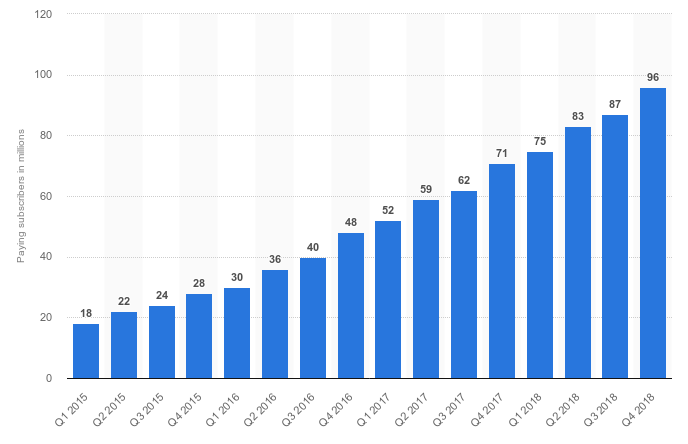
\includegraphics{Ethics/PayingSubscribers.png}
\centering
\caption{Spotify Paying Subscribers in Millions from Q1 2015 to Q4 2018}
\label{PayingSubs}
\end{figure}

With the significant increase in spending on streaming service
subscriptions over physical media sales, and digital downloads, as in
Figure \ref{StreamBecomesRiver}, the fair and equal payment of artists
must be considered. Artists of more niche genres can be negatively
affected by the currently used ``pro-rata'' models, however, the change
to a ``user-centric'' model may not benefit these artists, as they
increase the processing costs at the side of the streaming service. As
such, care must be taken to ensure that artists incomes are not so
negatively affected so as to reduce the number of smaller artists within
the industry.

\begin{figure}[H]
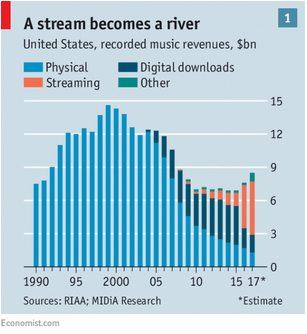
\includegraphics{Ethics/StreamBecomesRiver.png}
\centering
\caption{Recorded Music Revenues for the United States \cite{SpotPay18}}
\label{StreamBecomesRiver}
\end{figure}

\subsection{Audio Piracy}\label{audio-piracy}

When considering solutions which use locally stored audio, the ethical
issue of sourcing these audio tracks must be discussed. While it may be
presumed that, with the increase in the availability of audio streaming,
audio piracy would significantly decrease, it has been noted that audio
piracy affects physical and digital media
consumption\cite{onlinePiracy}. While the Global Online Piracy
Study\cite{onlinePiracy} suggests that audio piracy is decreasing, MUSO,
a company aiming to study and solve issues with audio piracy, has stated
in their annual piracy report a 1.6\% increase in global piracy in
2017\cite{muso}. Joost and Quintais however contest these figures,
noting that MUSO ``overestimate the number of and visits to pirate
websites''\cite{onlinePiracy}.

While piracy via illegal downloads seems to be decreasing, only
replacing the declining digital and physical sales\cite{SpotPay18},
illegal streaming via personal licences being used in place of business
licences may be a more prominent issue, with a survey showing 83\% of
small business owners use a personal streaming service account in their
premises\cite{licence}.

Sourcing audio files from legal sources, such as physical or online
retailers, is important in order to ensure proper payment is received by
artists and production companies. The use of locally stored audio in
this project may however increase the use of pirated audio, due to a
lack of accessibility to these physical or digital media.

\section{Listener Tracking}\label{listener-tracking-3}

Mobile tracking has a number of ethical implications, imposing on an
individuals right to privacy. Access to a users location data must be
privileged, accessible only when necessary, and only from the
application requiring the data. Bluetooth beacons, as used within this
project, have the capacity for two-way communication. As such, there is
the concern of the information being intercepted, which could lead to
malicious use of the captured data\cite{bleprivacy}.

As proximity based services become more common, it becomes increasingly
important to ensure the protection of a users personal data, and
location information. Both the Apple App Store, and Google Play Store
require that any application which requires access to location services,
or to bluetooth services request permission from the user to access
these services. This allows users the ability to block applications
accessing this information. Furthermore, laws have been introduced
prohibiting companies from using personal data from non-consenting
users\cite{proxmarketing}. Transparency is required throughout the
privacy policies of applications and services, in order to correctly
inform users of the data being accessed, and the storage and usage
conditions of this data.

\chapter{Conclusions and
Recommendations}\label{conclusions-and-recommendations}

\section{Conclusions}\label{conclusions}

\section{Recommendations}\label{recommendations}

\chapter{\texorpdfstring{Appendix
\label{Appendix}}{Appendix }}\label{appendix}

\section{\texorpdfstring{Audio Server Software Munin Data
\label{MuninData}}{Audio Server Software Munin Data }}\label{audio-server-software-munin-data}

\subsection{MPD}\label{mpd-2}

\textbf{Disk}

\begin{figure}[H]
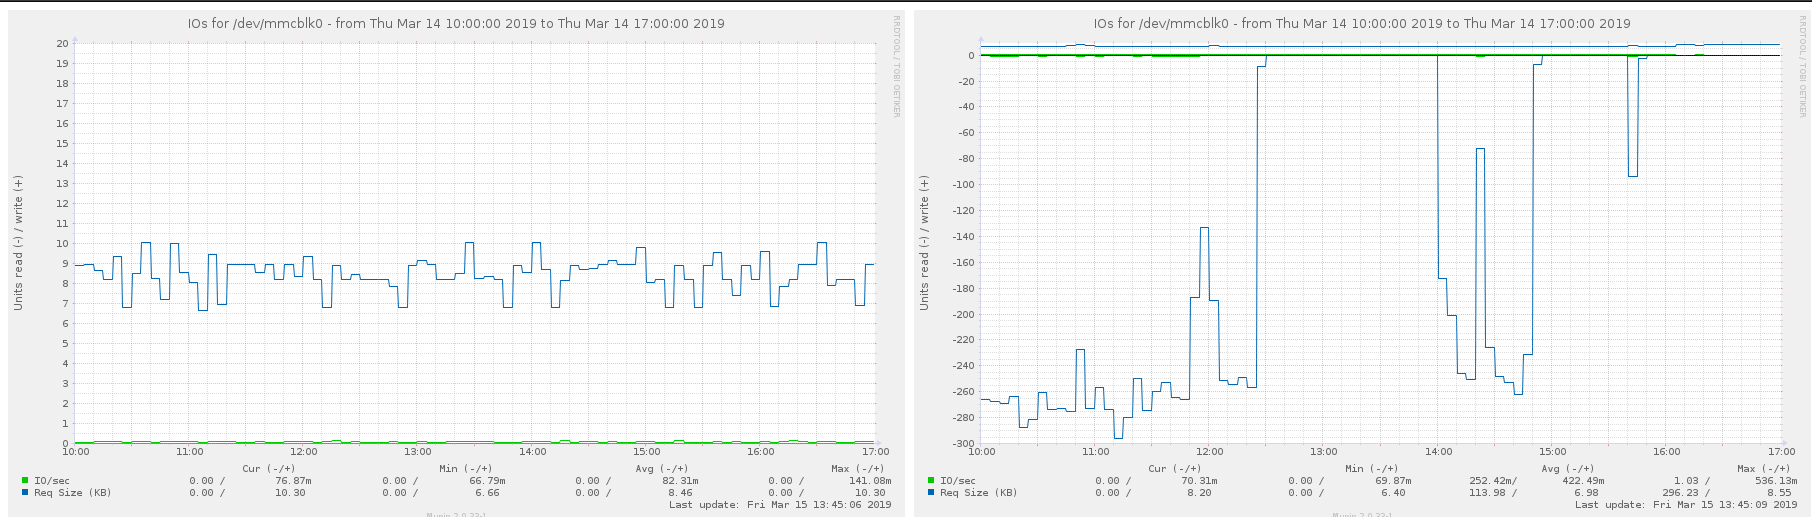
\includegraphics{ResultsAndAnalysis/MPDServerTestImages/005MPDDiskIO.png}
\centering
\caption{MPD Disk I/O on Client and Server Device}
\label{MPDDiskIO}
\end{figure}

\begin{figure}[H]
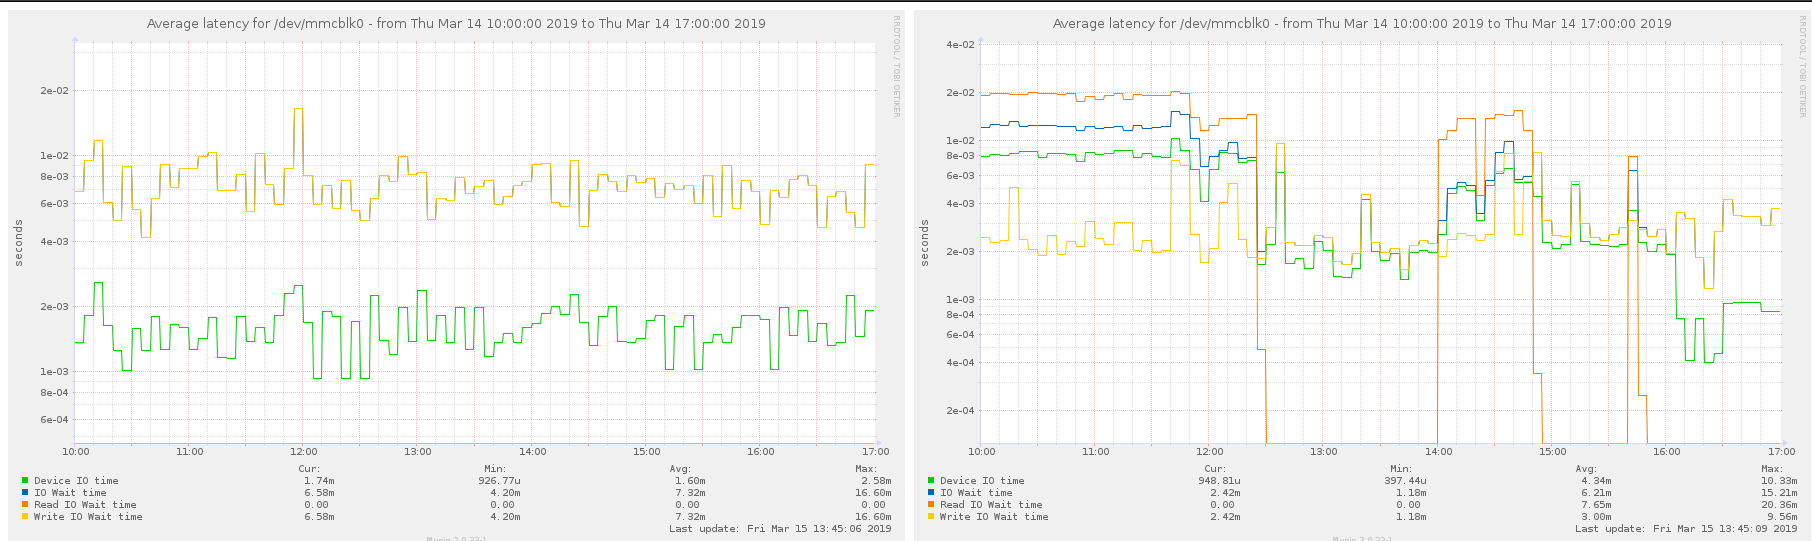
\includegraphics{ResultsAndAnalysis/MPDServerTestImages/006MPDDiskLatency.png}
\centering
\caption{MPD Client and Server Device Disk Latency}
\label{MPDDiskLatency}
\end{figure}

\begin{figure}[H]
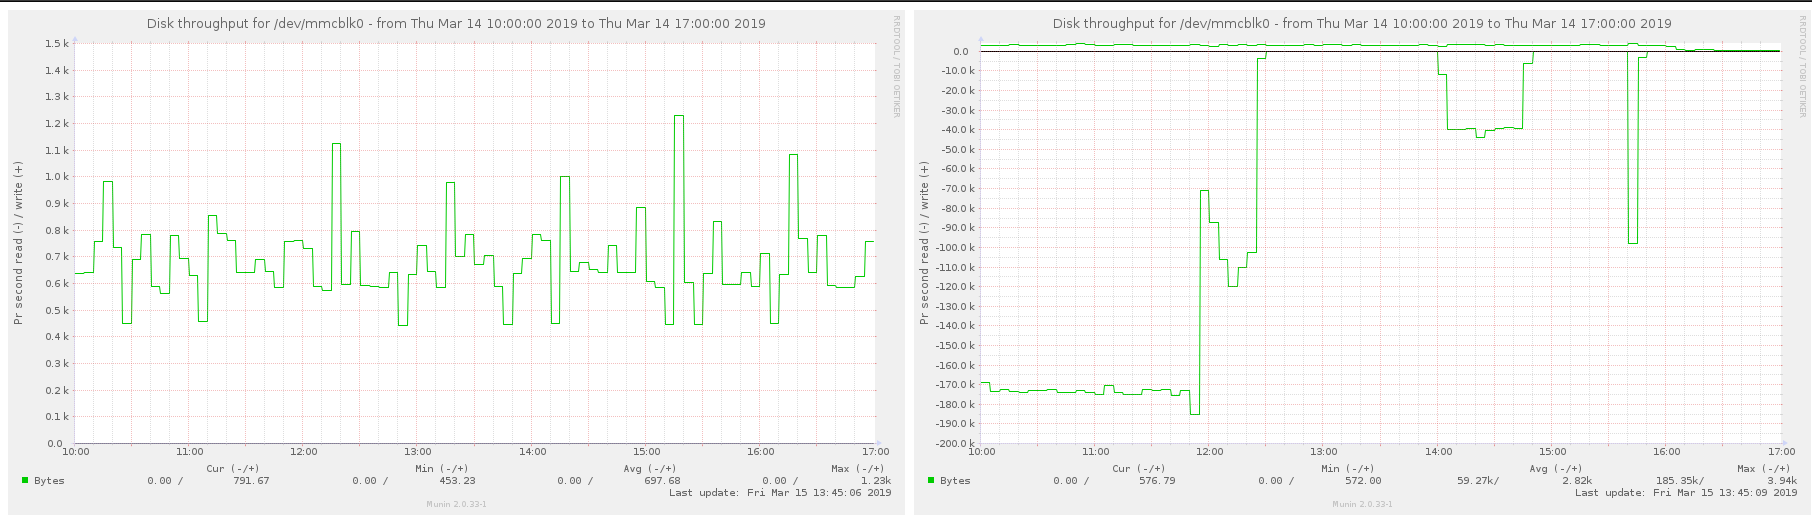
\includegraphics{ResultsAndAnalysis/MPDServerTestImages/007MPDDiskThroughput.png}
\centering
\caption{MPD Client and Server Device Disk Throughput}
\label{MPDDiskThroughput}
\end{figure}

\begin{figure}[H]
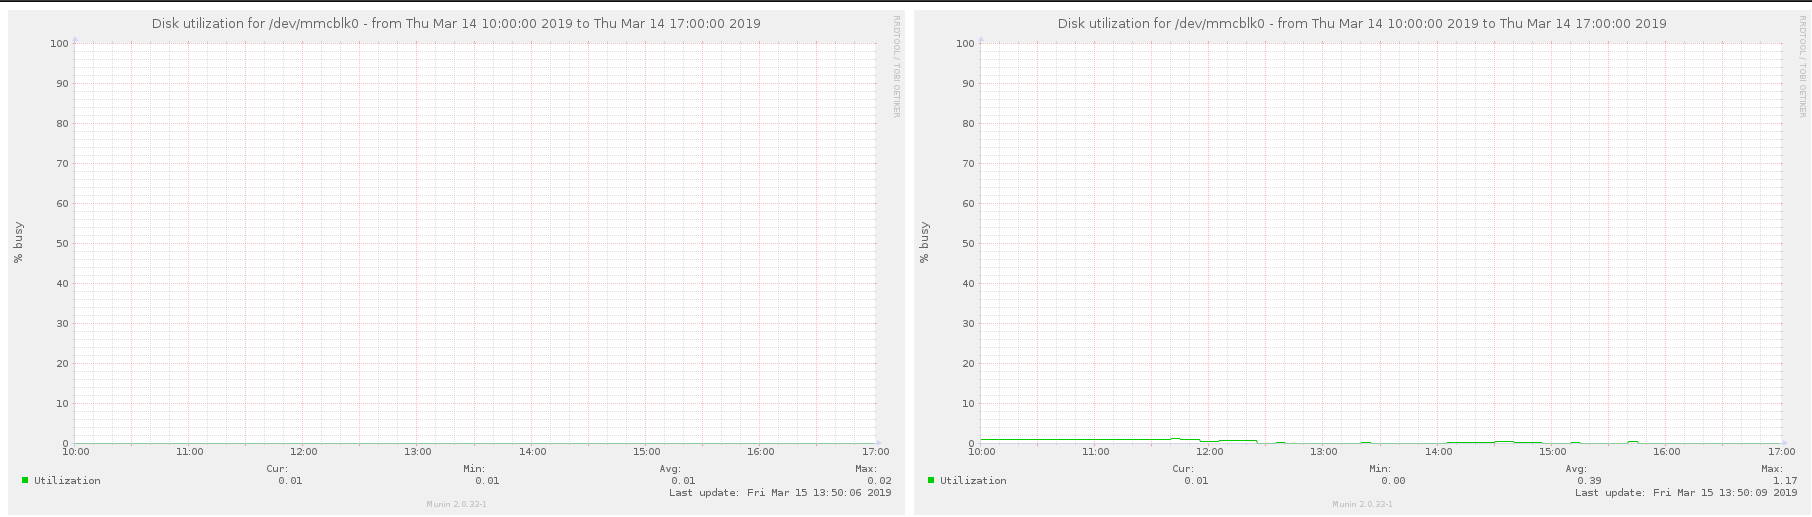
\includegraphics{ResultsAndAnalysis/MPDServerTestImages/008MPDDiskUtilization.png}
\centering
\caption{MPD Client and Server Device Disk Utilization}
\label{MPDDiskUtil}
\end{figure}

\textbf{Network}

\begin{figure}[H]
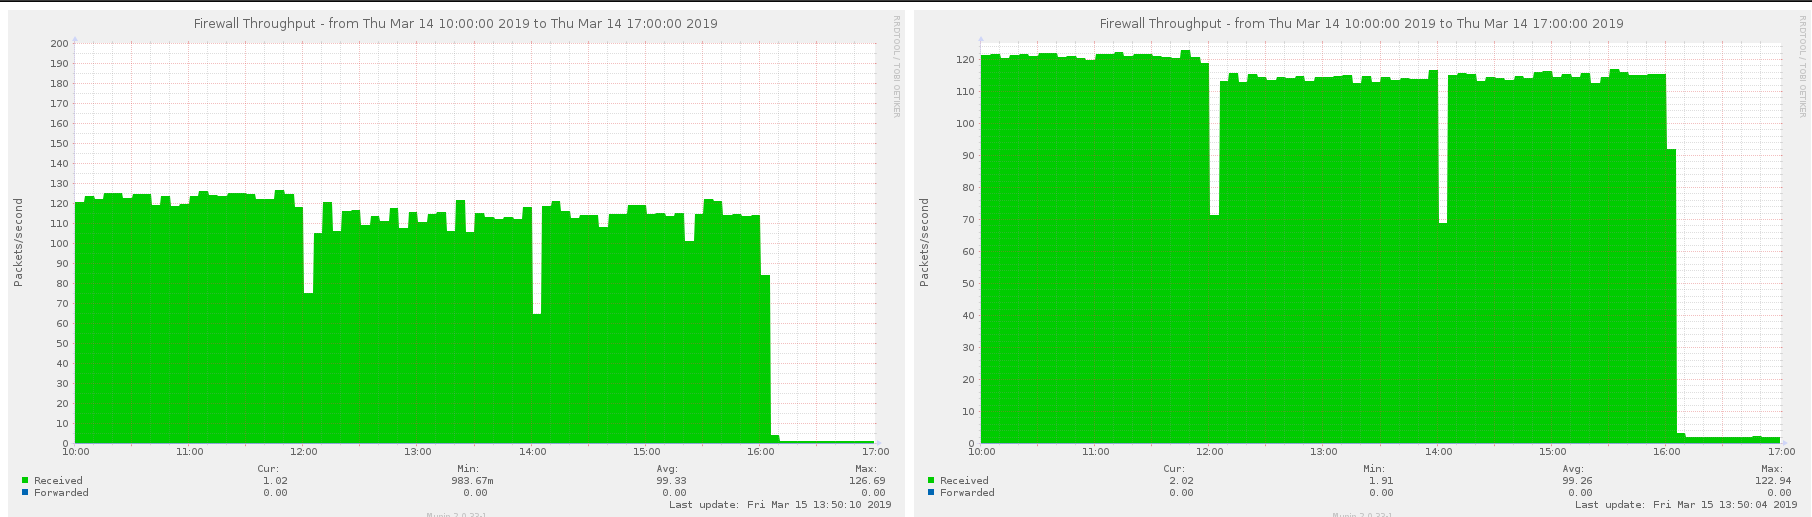
\includegraphics{ResultsAndAnalysis/MPDServerTestImages/011MPDFirewallThroughput.png}
\centering
\caption{MPD Client and Server Device Firewall Throughput}
\label{MPDFirewallThroughput}
\end{figure}

\begin{figure}[H]
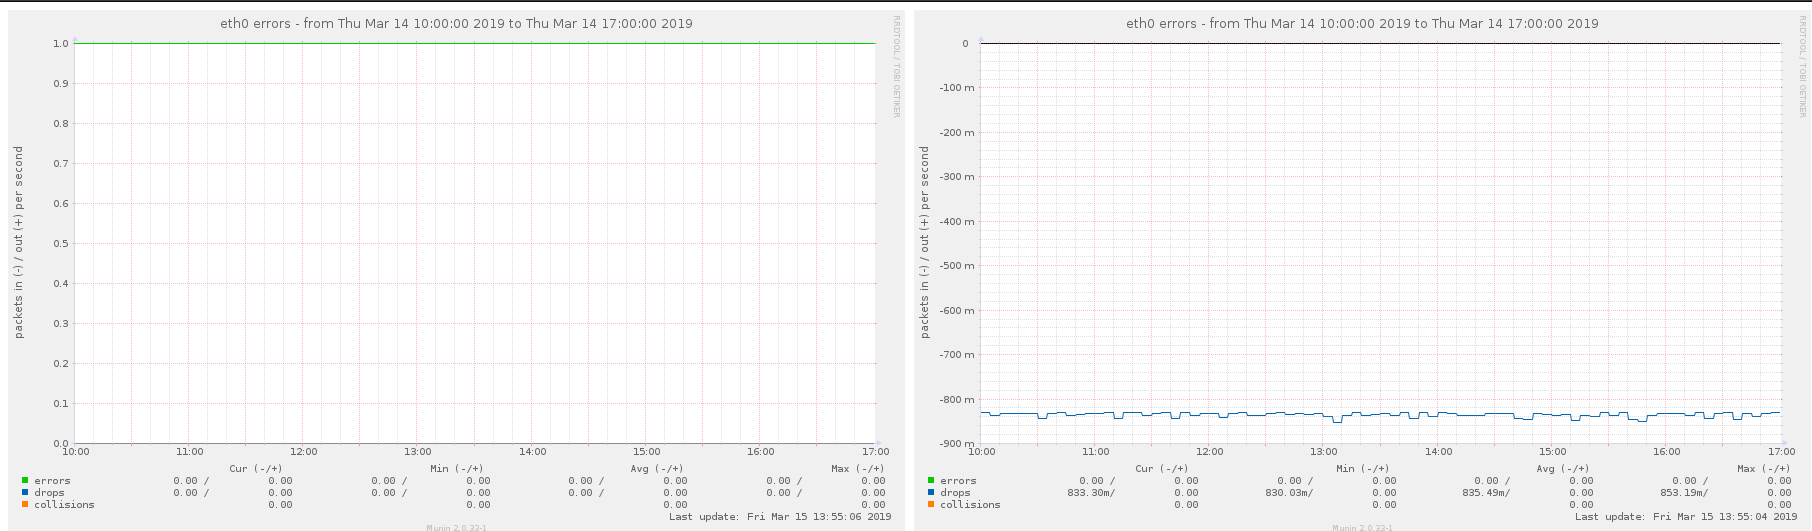
\includegraphics{ResultsAndAnalysis/MPDServerTestImages/009MPDEth0Errors.png}
\centering
\caption{MPD Client and Server Device Eth Errors}
\label{MPDEthError}
\end{figure}

\begin{figure}[H]
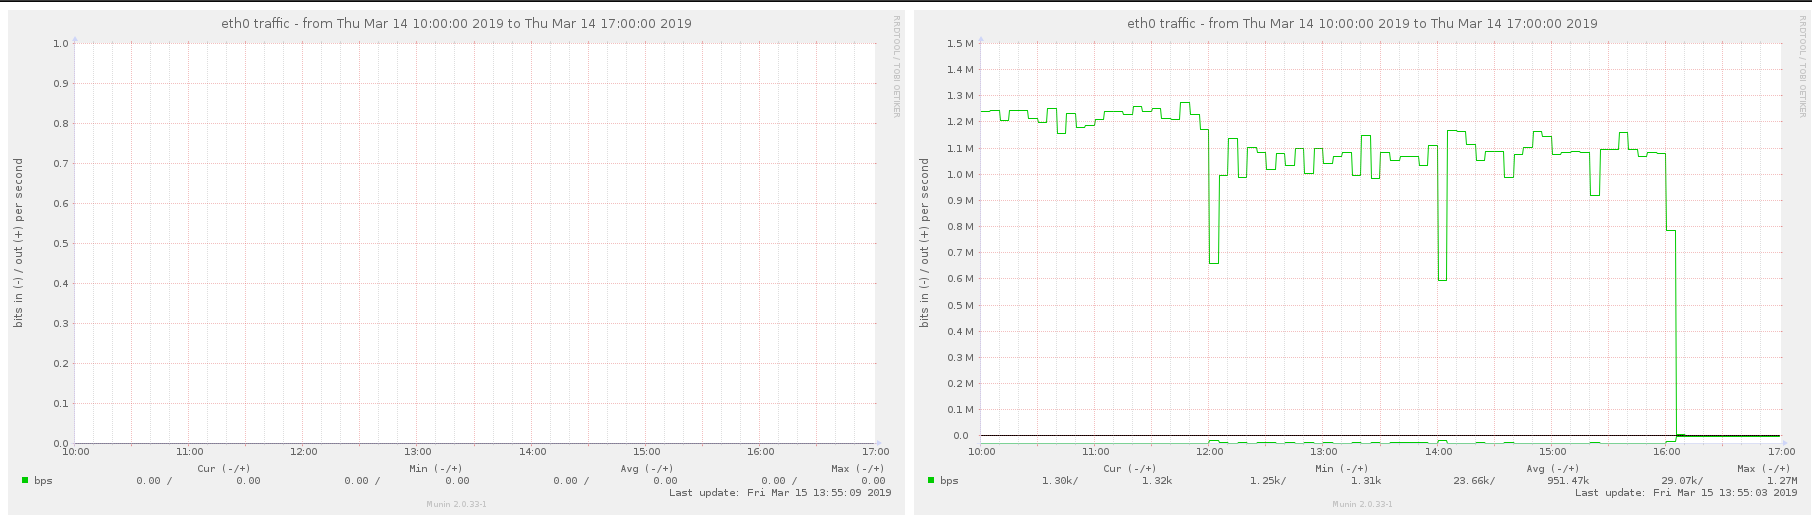
\includegraphics{ResultsAndAnalysis/MPDServerTestImages/010MPDEth0Traffic.png}
\centering
\caption{MPD Client and Server Device Eth Traffic}
\label{MPDEthTraffic}
\end{figure}

\begin{figure}[H]
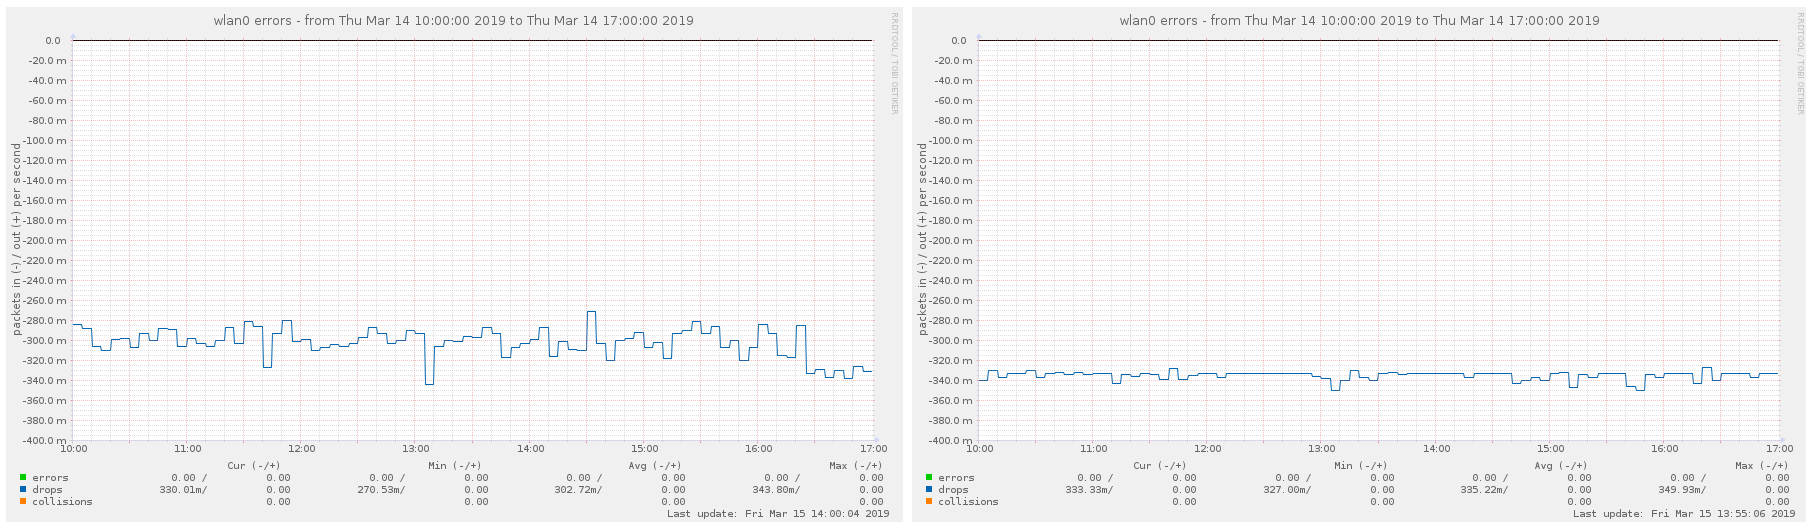
\includegraphics{ResultsAndAnalysis/MPDServerTestImages/020MPDWlan0Errors.png}
\centering
\caption{MPD Client and Server Device Wlan Errors}
\label{MPDWlanError}
\end{figure}

\begin{figure}[H]
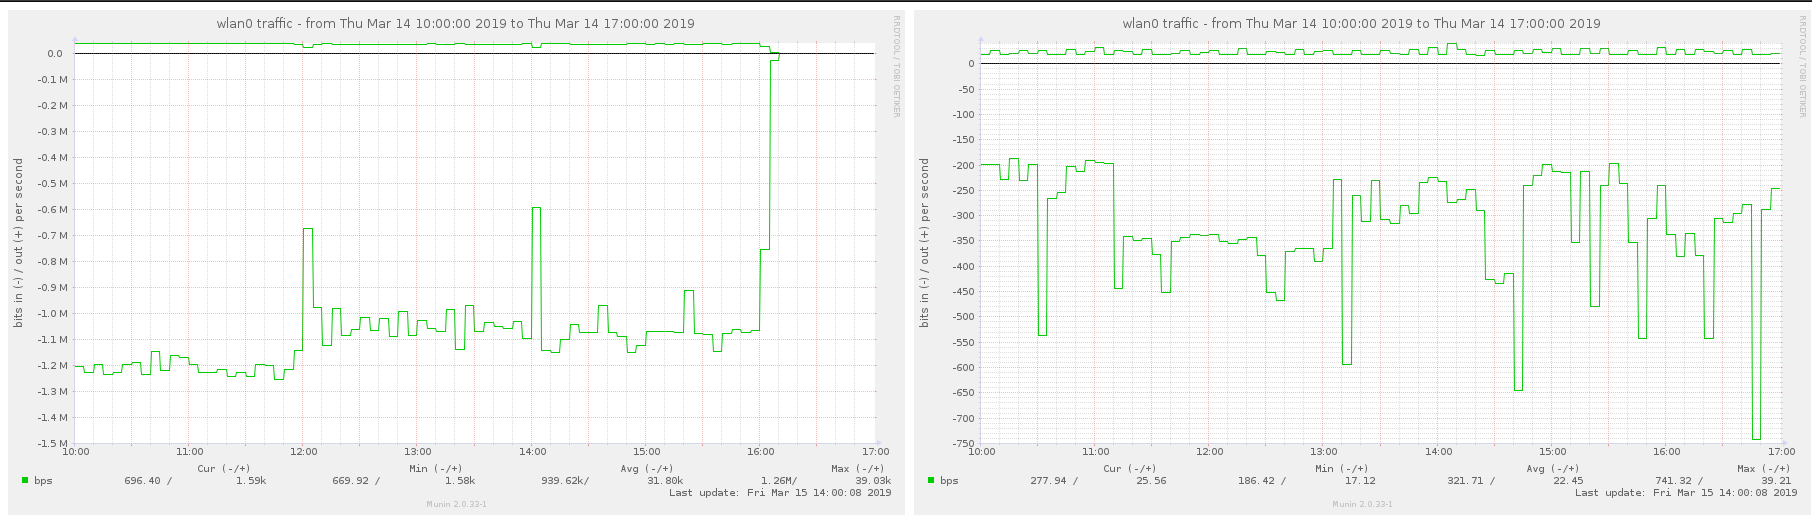
\includegraphics{ResultsAndAnalysis/MPDServerTestImages/021MPDWlan0Traffic.png}
\centering
\caption{MPD Client and Server Device Wlan Traffic}
\label{MPDWlanTraffic}
\end{figure}

\begin{figure}[H]
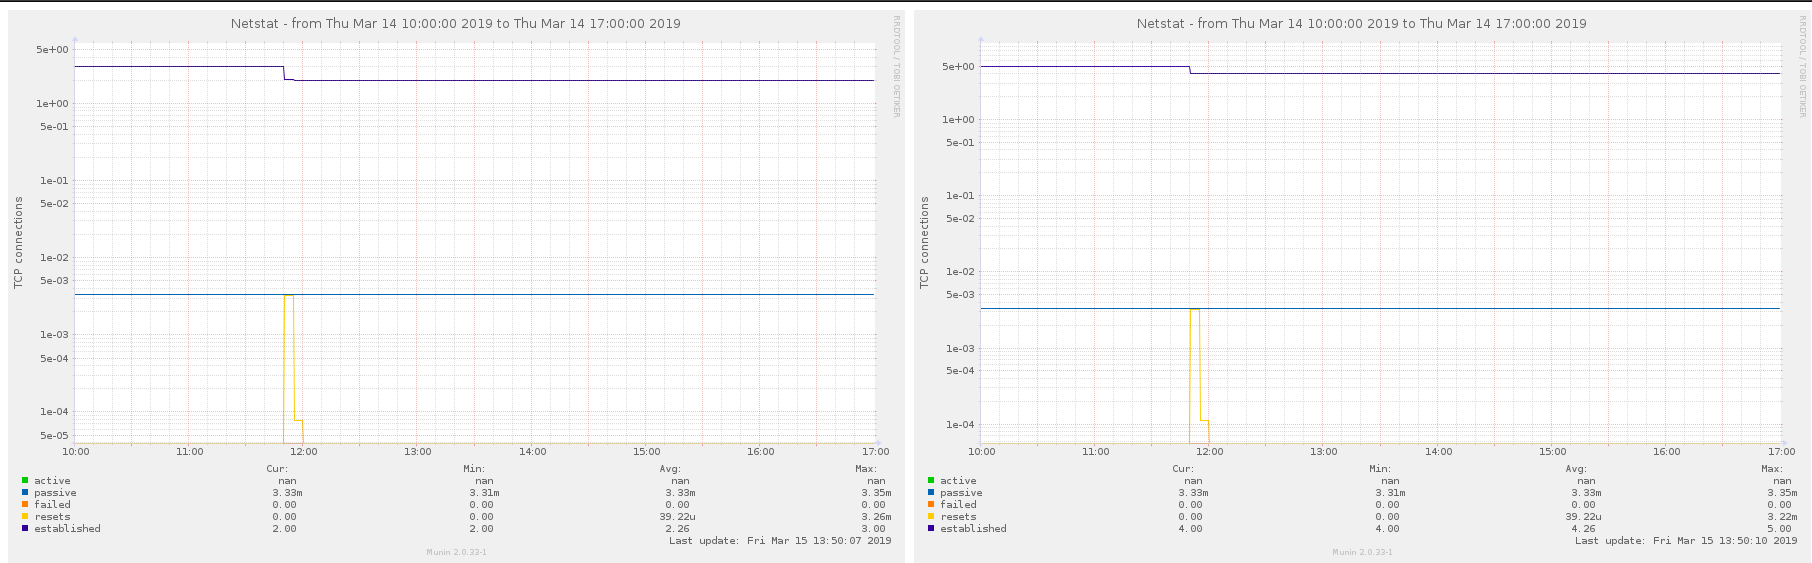
\includegraphics{ResultsAndAnalysis/MPDServerTestImages/017MPDNetstat.png}
\centering
\caption{MPD Client and Server Device Netstat}
\label{MPDNetstat}
\end{figure}

\textbf{Processes}

\begin{figure}[H]
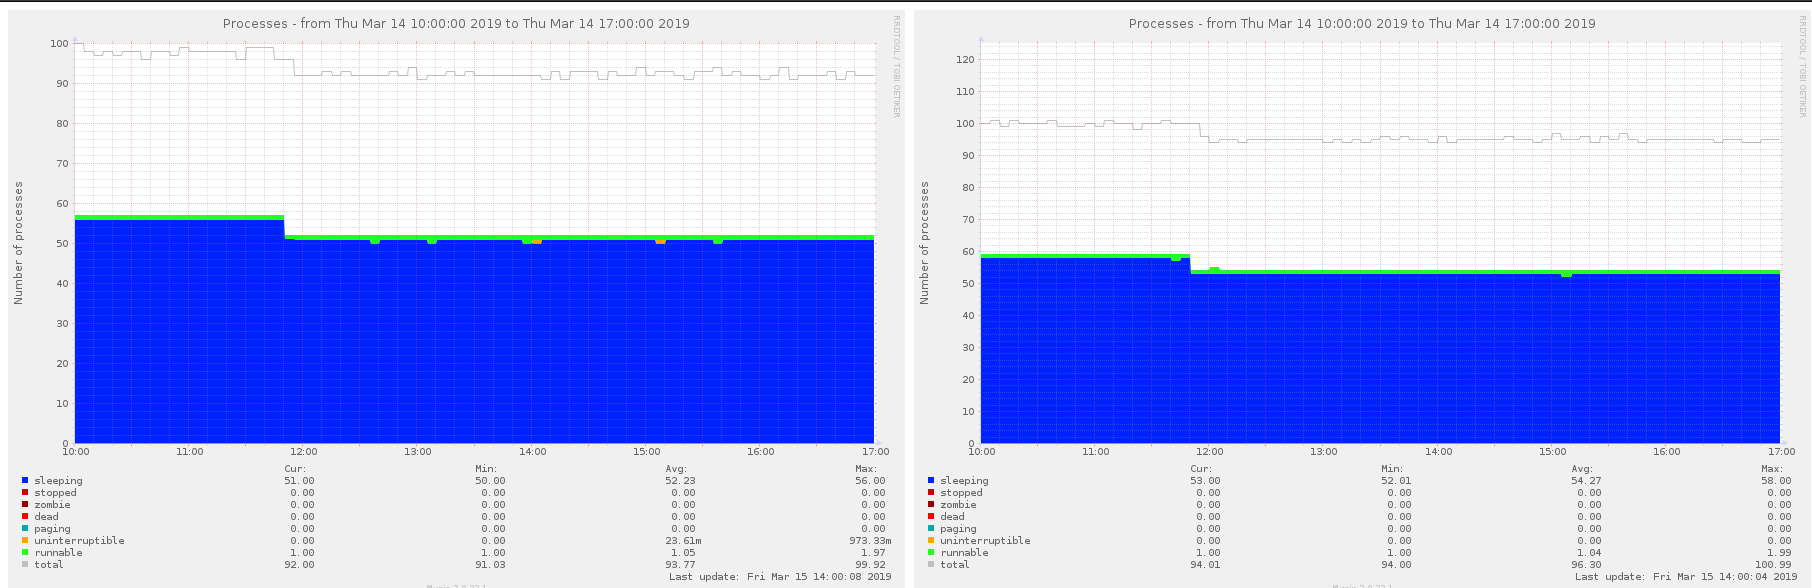
\includegraphics{ResultsAndAnalysis/MPDServerTestImages/019MPDProcesses.png}
\centering
\caption{MPD Client and Server Device Processes}
\label{MPDProcesses}
\end{figure}

\begin{figure}[H]
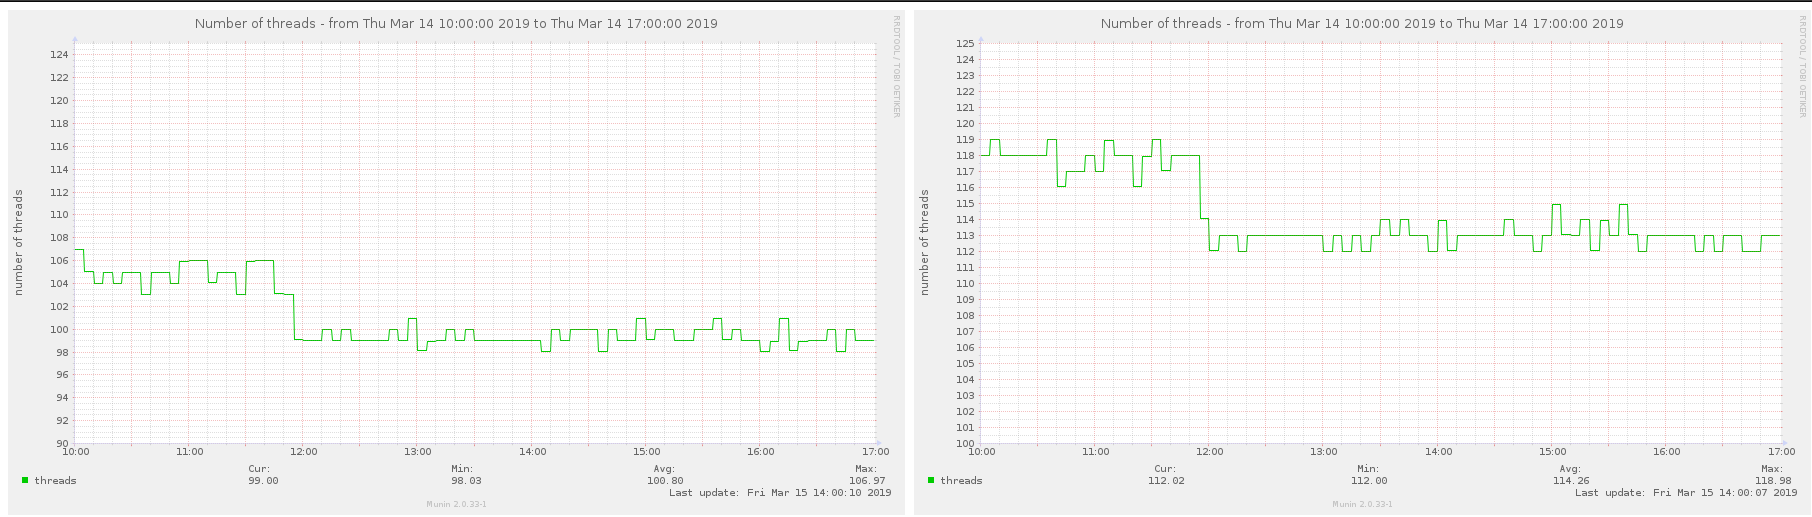
\includegraphics{ResultsAndAnalysis/MPDServerTestImages/018MPDNoOfThreads.png}
\centering
\caption{MPD Client and Server Device Number of Threads}
\label{MPDNumThreads}
\end{figure}

\textbf{System}

\begin{figure}[H]
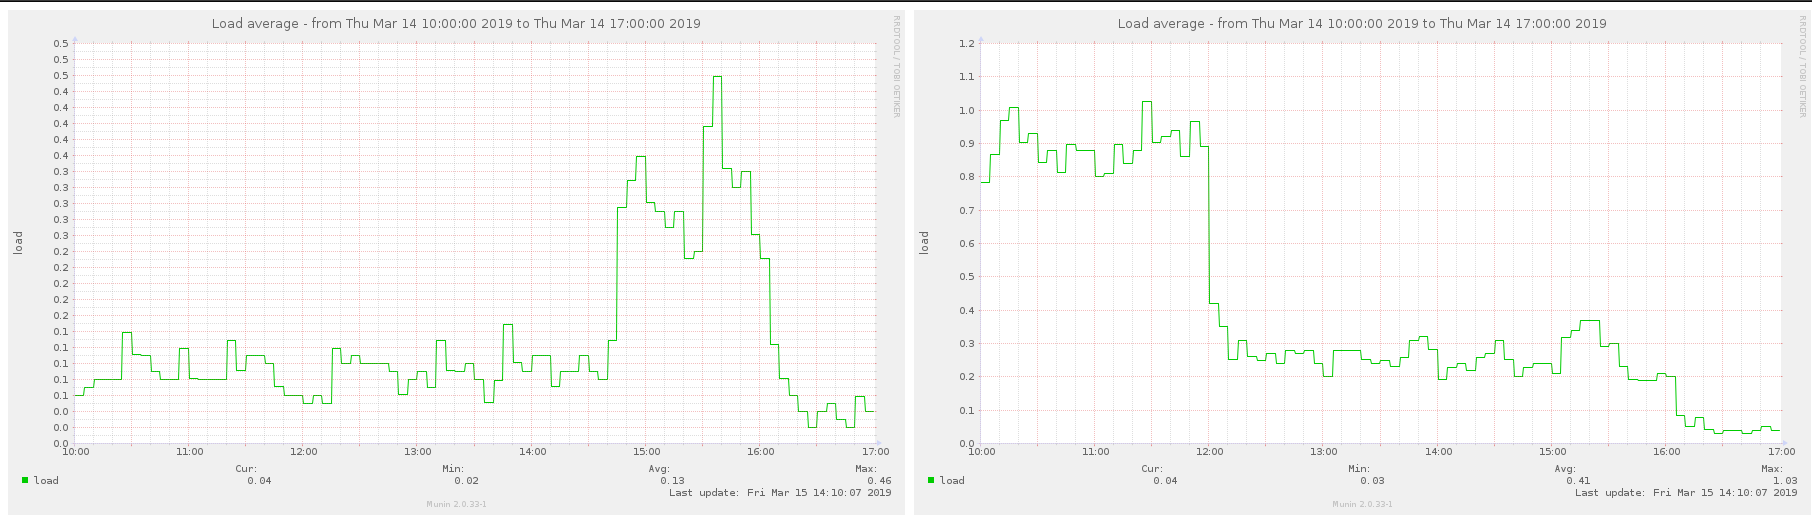
\includegraphics{ResultsAndAnalysis/MPDServerTestImages/015MPDLoadAverage.png}
\centering
\caption{MPD Client and Server Device Load Average}
\label{MPDLoadAvg}
\end{figure}

\begin{figure}[H]
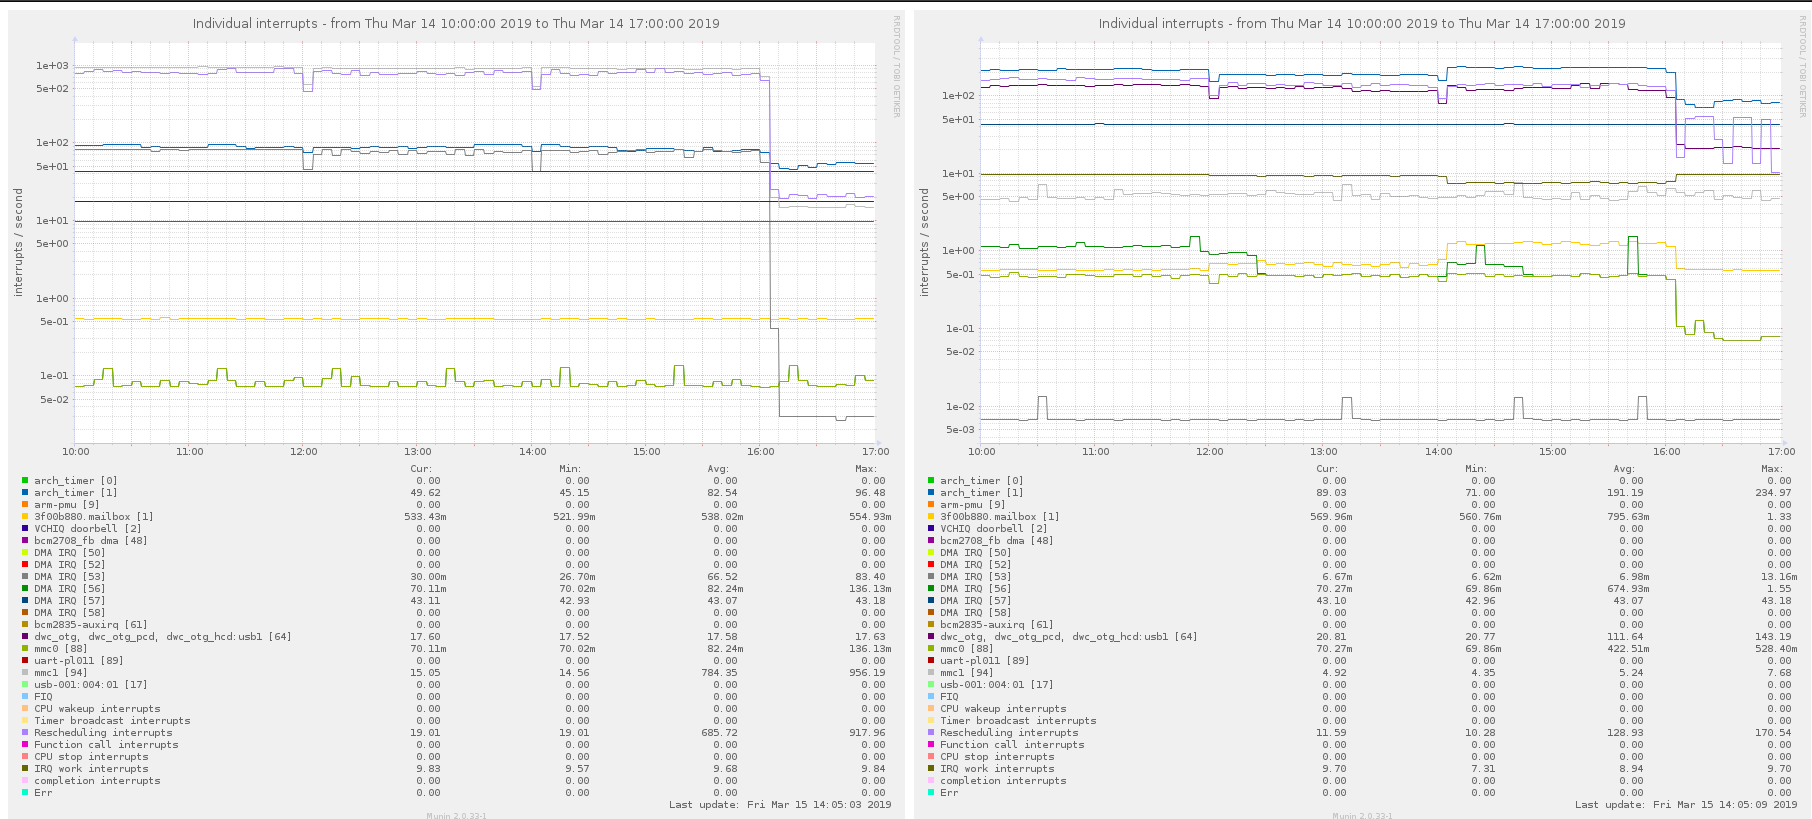
\includegraphics{ResultsAndAnalysis/MPDServerTestImages/013MPDIndividualInterrupts.png}
\centering
\caption{MPD Client and Server Device Individual Interrupts}
\label{MPDIndInt}
\end{figure}

\begin{figure}[H]
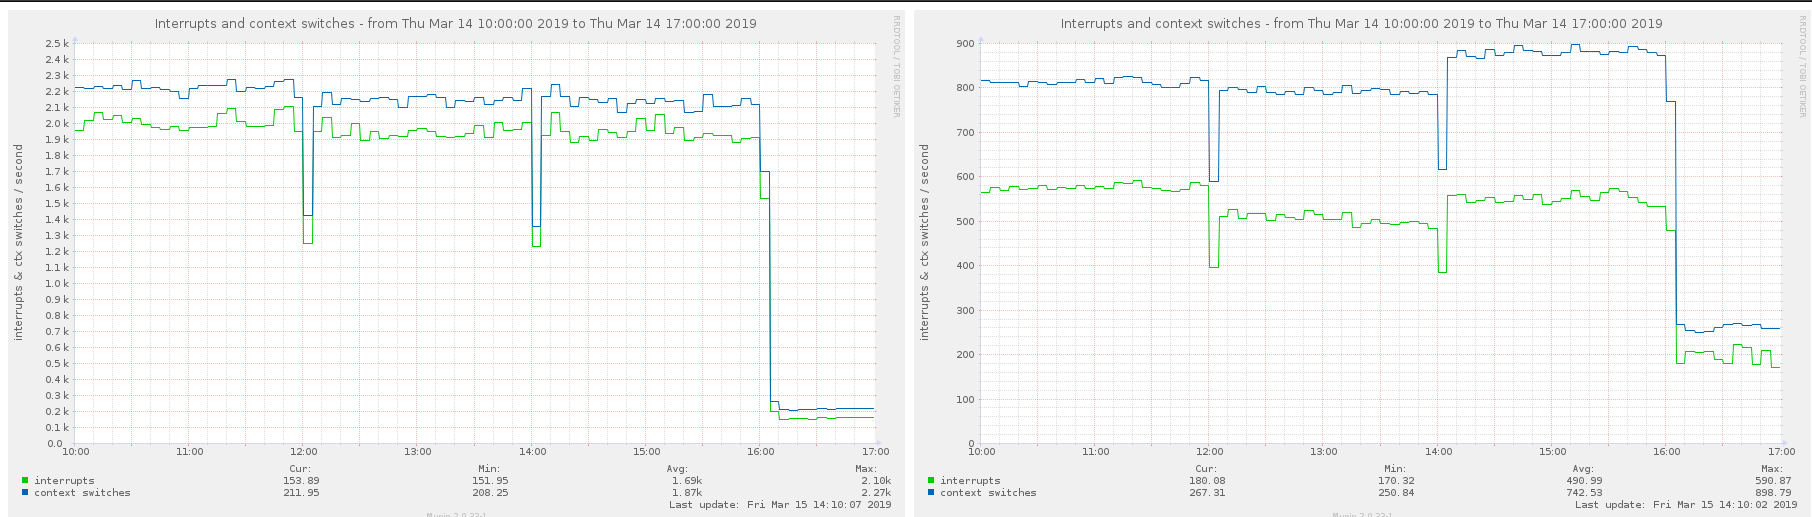
\includegraphics{ResultsAndAnalysis/MPDServerTestImages/014MPDInterruptsAndContextSwitches.png}
\centering
\caption{MPD Client and Server Device Interrupts and Context Switches}
\label{MPDIntCont}
\end{figure}

\begin{figure}[H]
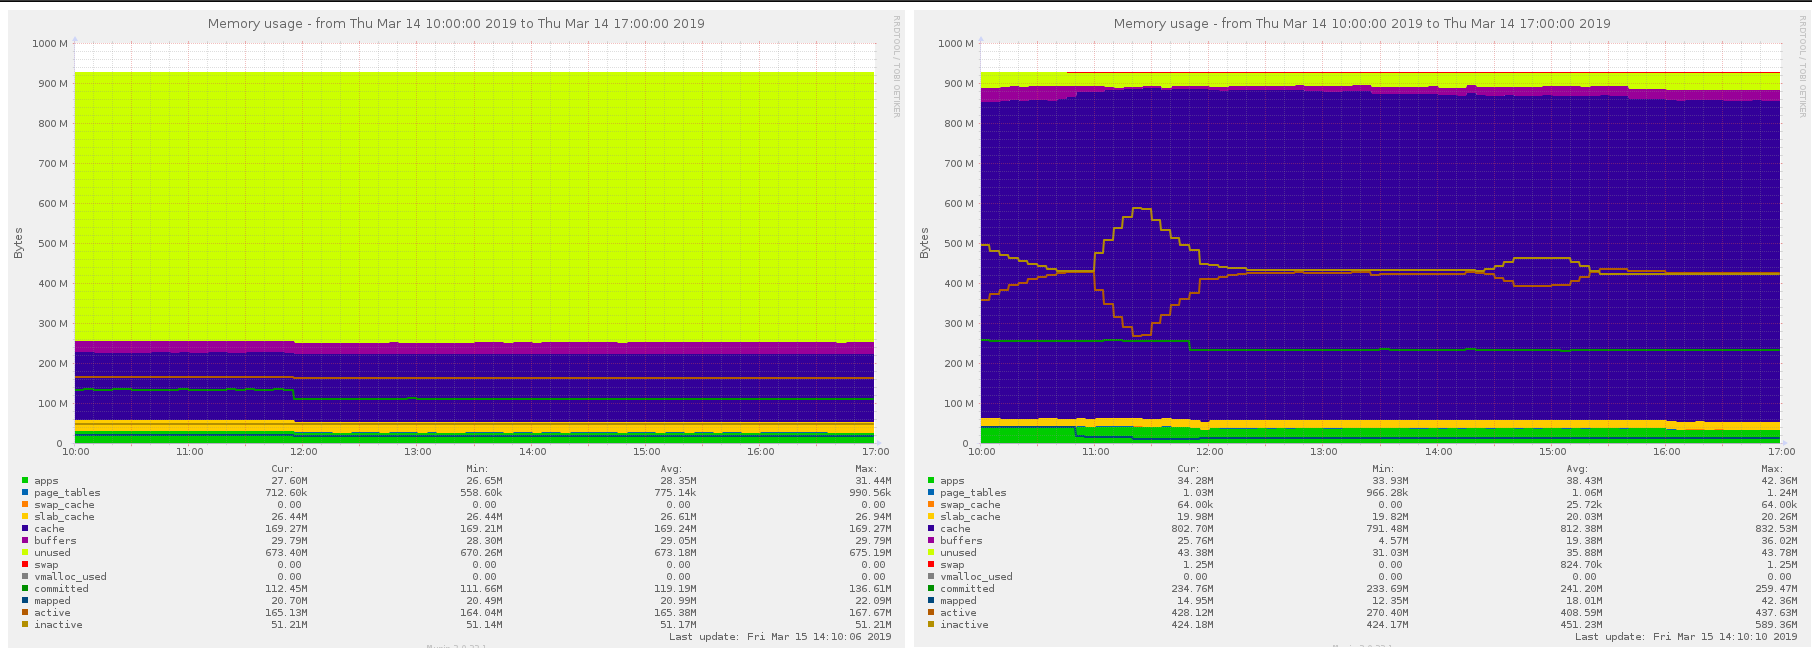
\includegraphics{ResultsAndAnalysis/MPDServerTestImages/016MPDMemoryUsage.png}
\centering
\caption{MPD Client and Server Device Memory Usage}
\label{MPDMemUse}
\end{figure}

\begin{figure}[H]
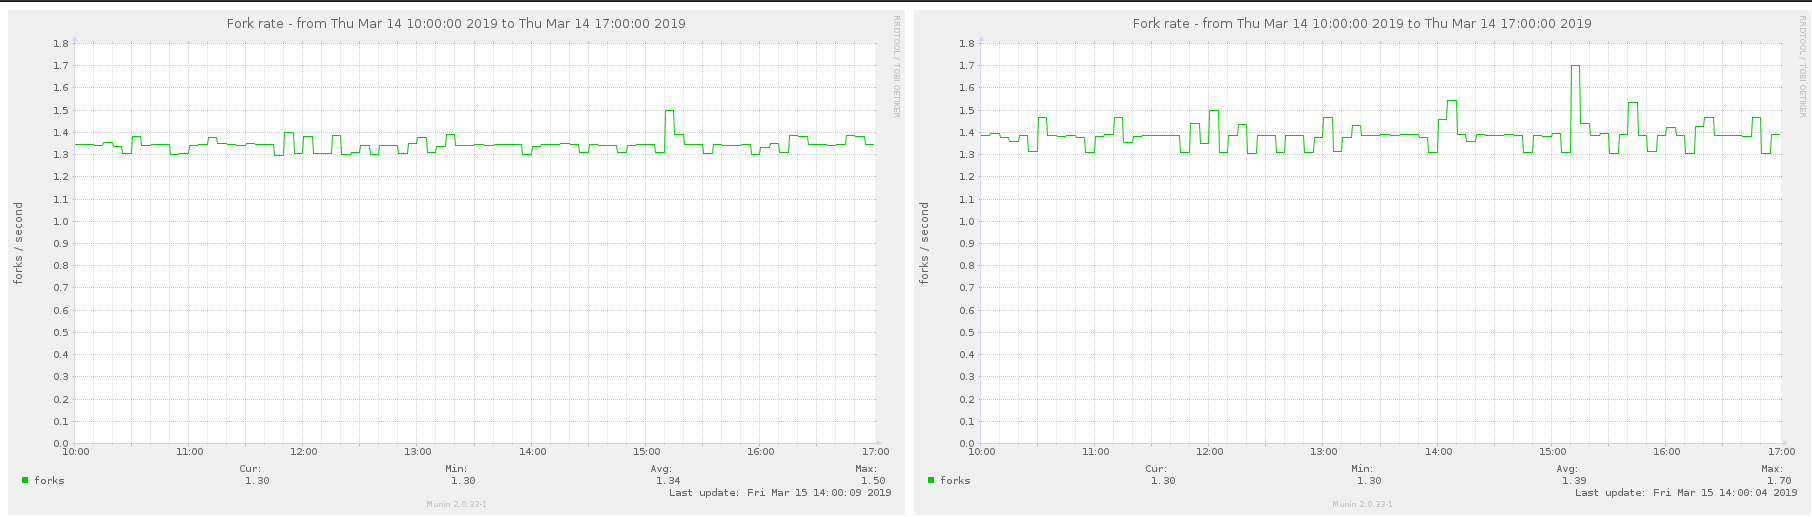
\includegraphics{ResultsAndAnalysis/MPDServerTestImages/012MPDForkRate.png}
\centering
\caption{MPD Client and Server Device Fork Rate}
\label{MPDForkRate}
\end{figure}

\begin{figure}[H]
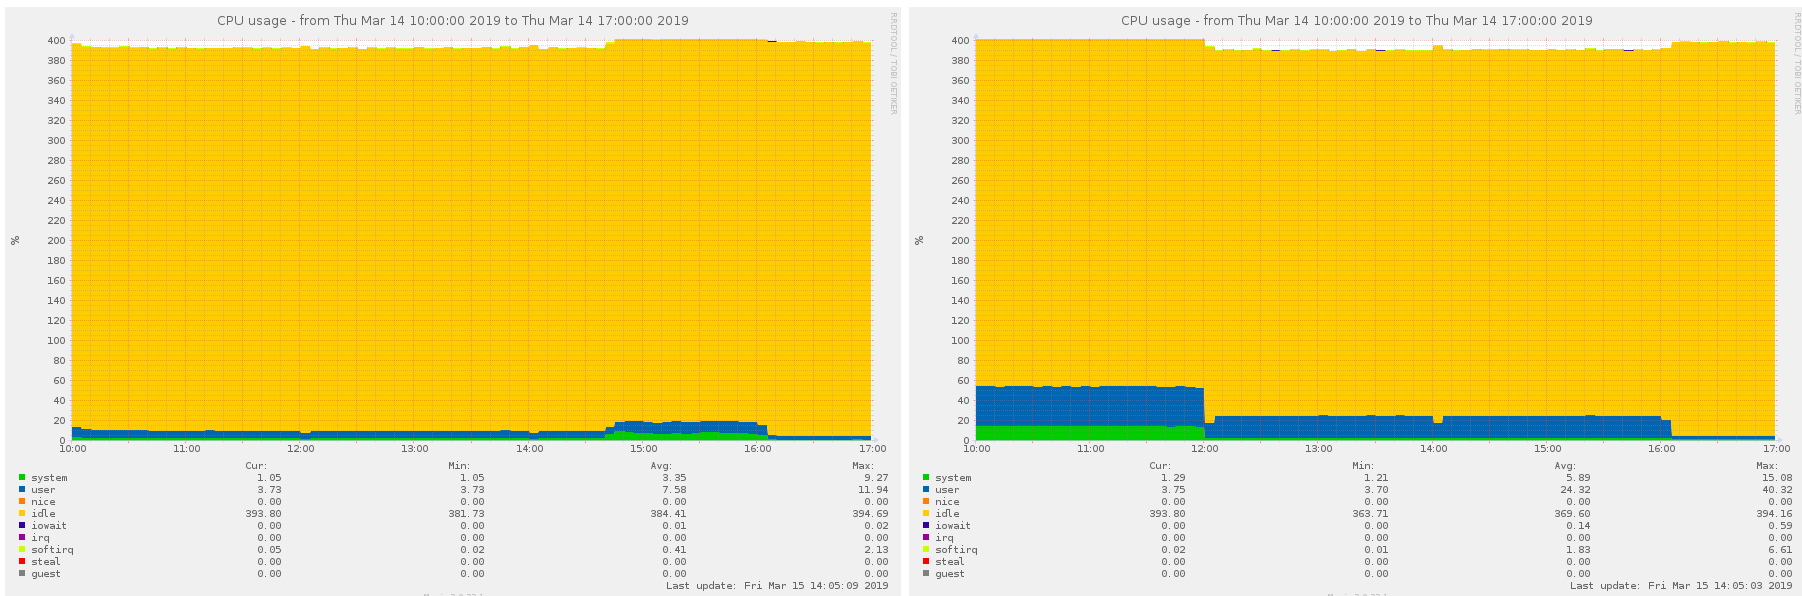
\includegraphics{ResultsAndAnalysis/MPDServerTestImages/004MPDCPUUsage.png}
\centering
\caption{MPD Client and Server Device CPU Usage}
\label{MPDCPUUsage}
\end{figure}

\textbf{Sensors}

\begin{figure}[H]
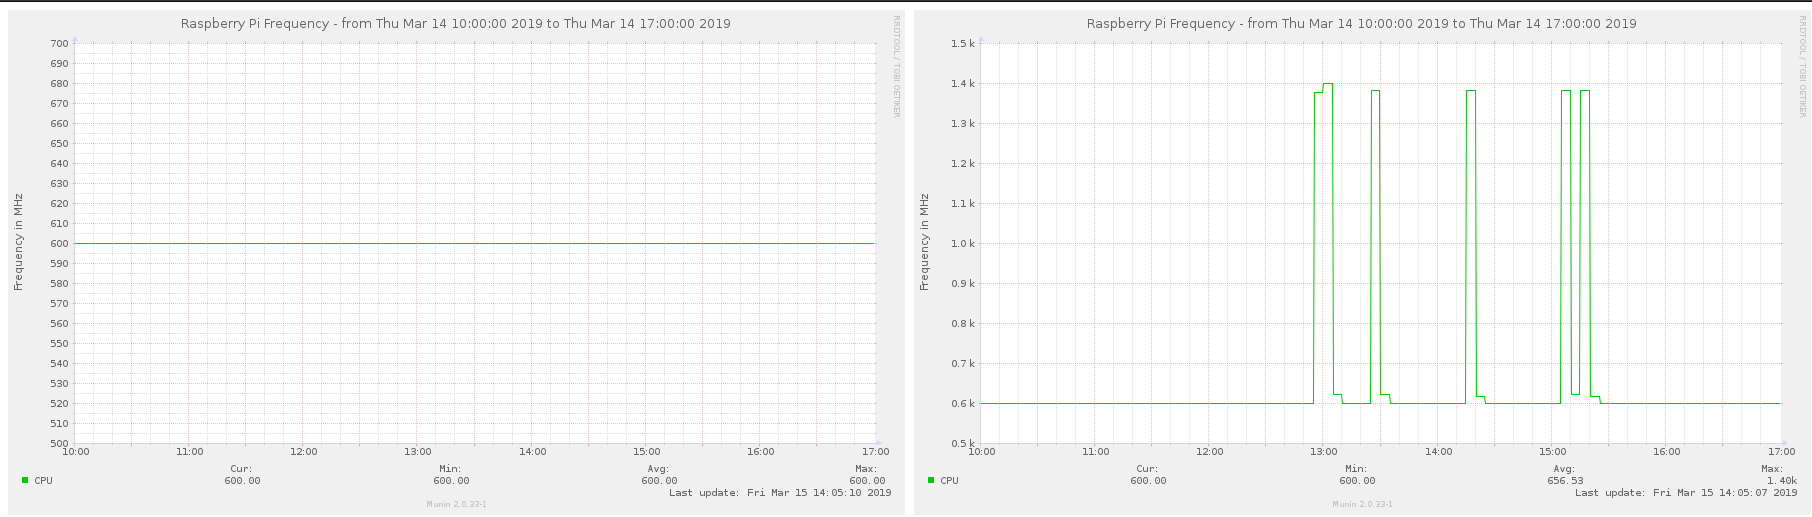
\includegraphics{ResultsAndAnalysis/MPDServerTestImages/001MPDCPUFreq.png}
\centering
\caption{MPD Client and Server Device CPU Frequency}
\label{MPDCPUFreq}
\end{figure}

\begin{figure}[H]
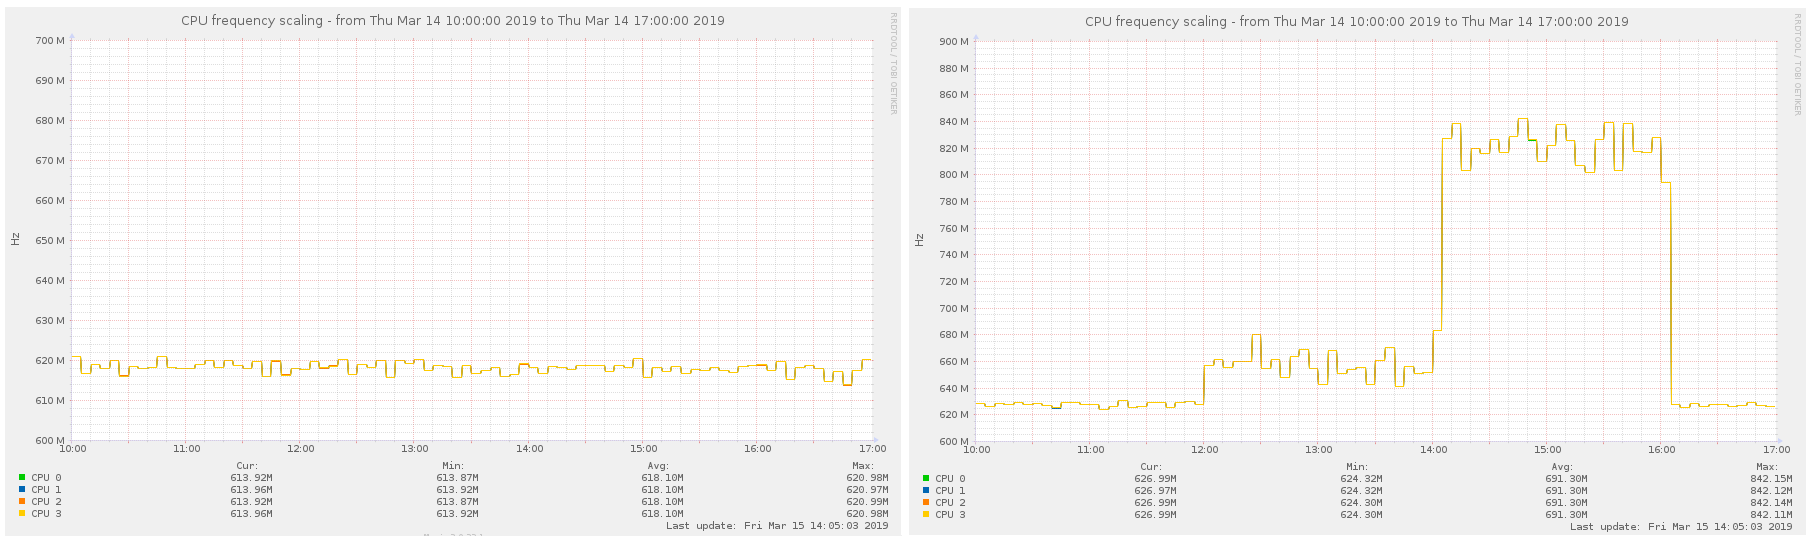
\includegraphics{ResultsAndAnalysis/MPDServerTestImages/002MPDCPUFreqScaling.png}
\centering
\caption{MPD Client and Server Device CPU Frequency Scaling}
\label{MPDCPUFreqScaling}
\end{figure}

\begin{figure}[H]
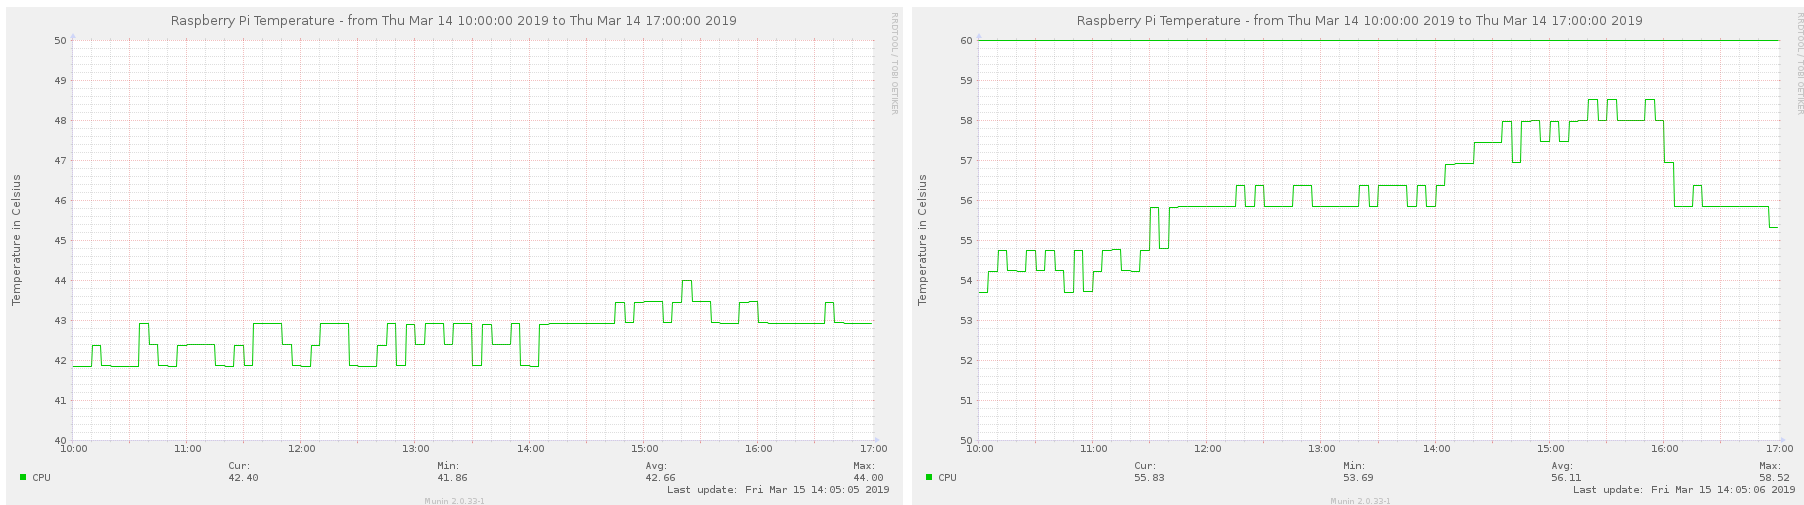
\includegraphics{ResultsAndAnalysis/MPDServerTestImages/003MPDCPUTemp.png}
\centering
\caption{MPD Client and Server Device CPU Temperature}
\label{MPDCPUTemp}
\end{figure}

\subsection{Mopidy}\label{mopidy-2}

\textbf{Disk}

\begin{figure}[H]
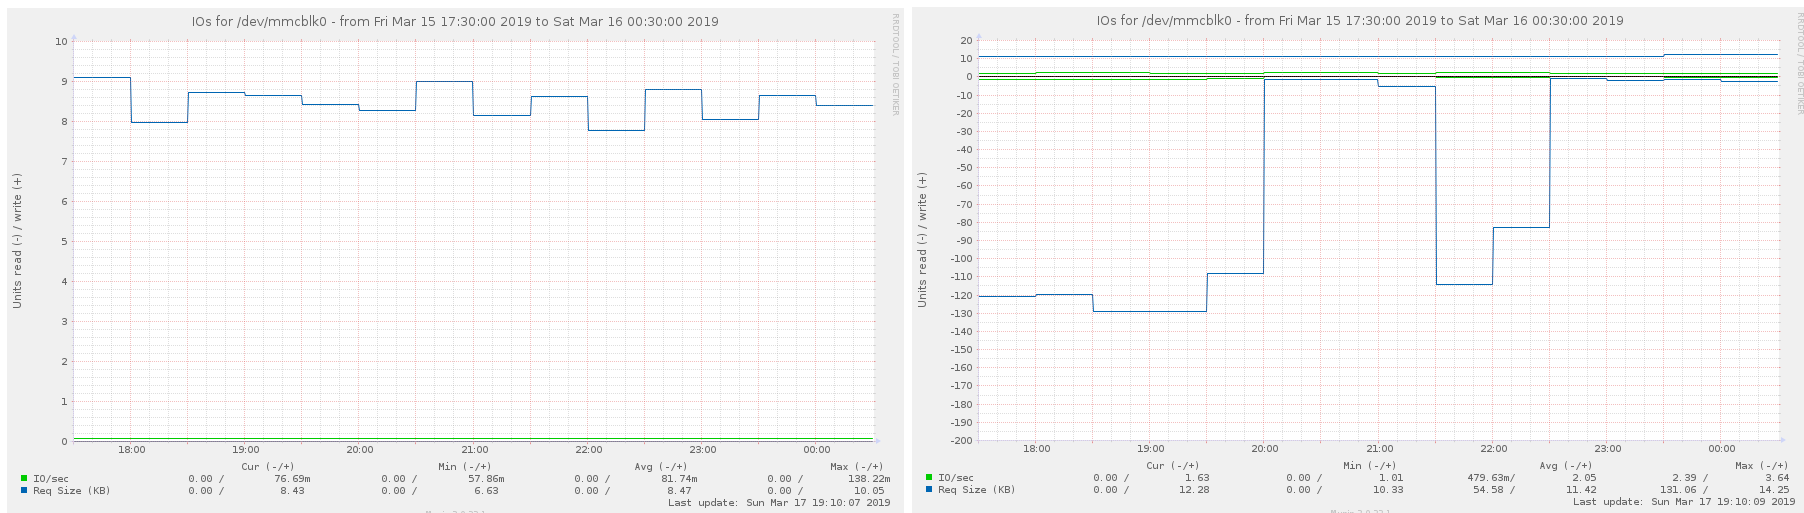
\includegraphics{ResultsAndAnalysis/MopidyServerTestImages/005MopidyDiskIO.png}
\centering
\caption{Mmopidy Disk I/O on Client and Server Device}
\label{MopidyDiskIO}
\end{figure}

\begin{figure}[H]
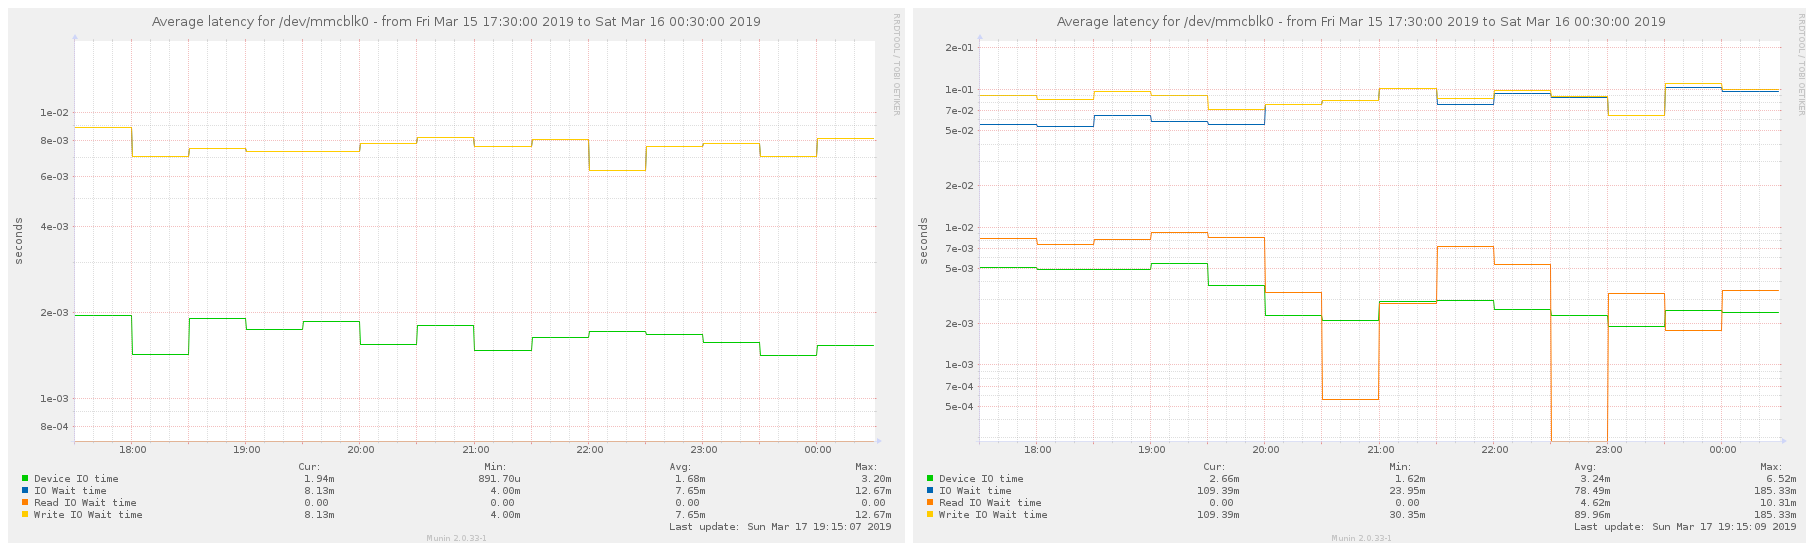
\includegraphics{ResultsAndAnalysis/MopidyServerTestImages/006MopidyDiskLatency.png}
\centering
\caption{Mopidy Client and Server Device Disk Latency}
\label{MopidyDiskLatency}
\end{figure}

\begin{figure}[H]
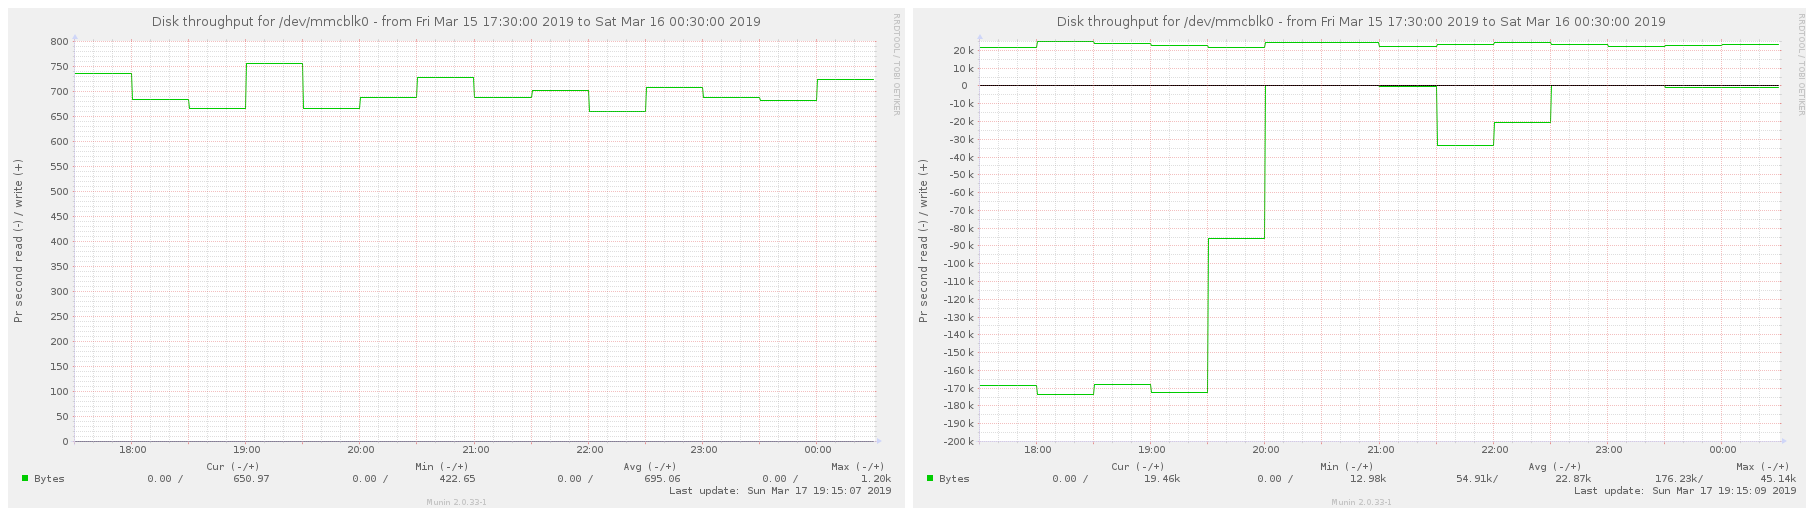
\includegraphics{ResultsAndAnalysis/MopidyServerTestImages/007MopidyDiskThroughput.png}
\centering
\caption{Mopidy Client and Server Device Disk Throughput}
\label{MopidyDiskThroughput}
\end{figure}

\begin{figure}[H]
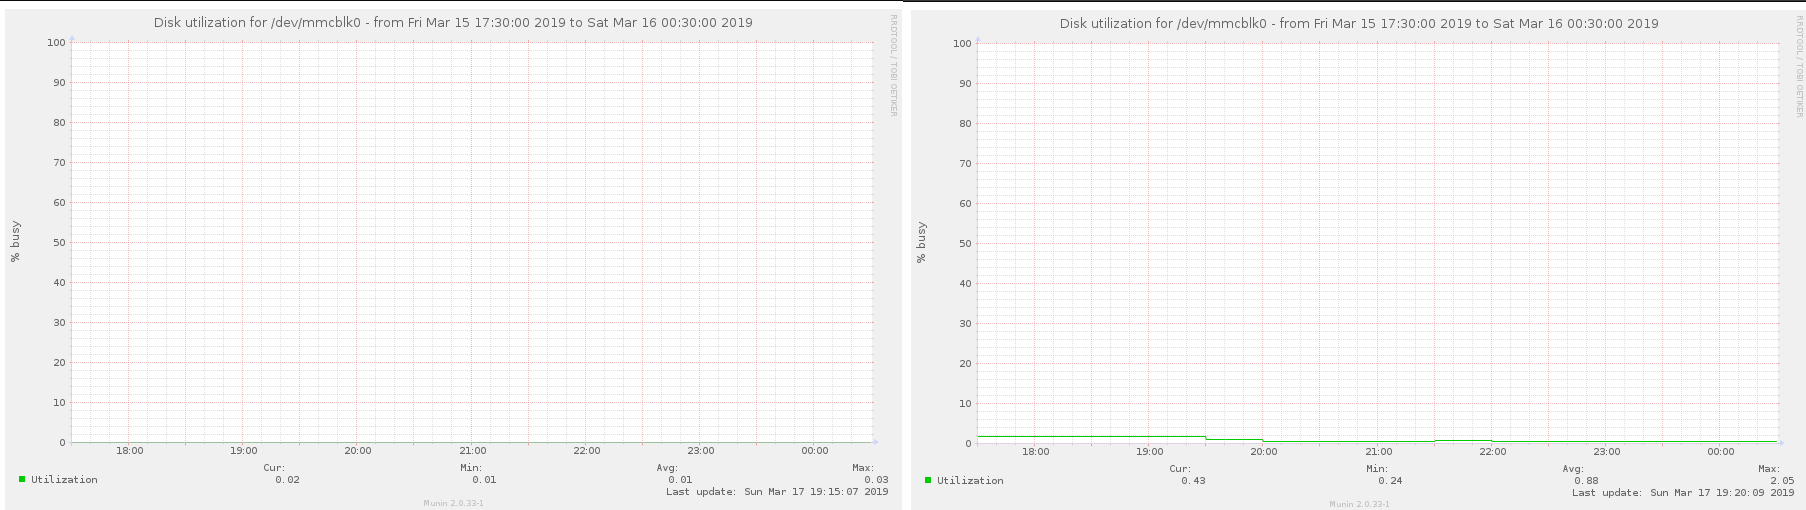
\includegraphics{ResultsAndAnalysis/MopidyServerTestImages/009MopidyDiskUtilization.png}
\centering
\caption{Mopidy Client and Server Device Disk Utilization}
\label{MopidyDiskUtil}
\end{figure}

\textbf{Network}

\begin{figure}[H]
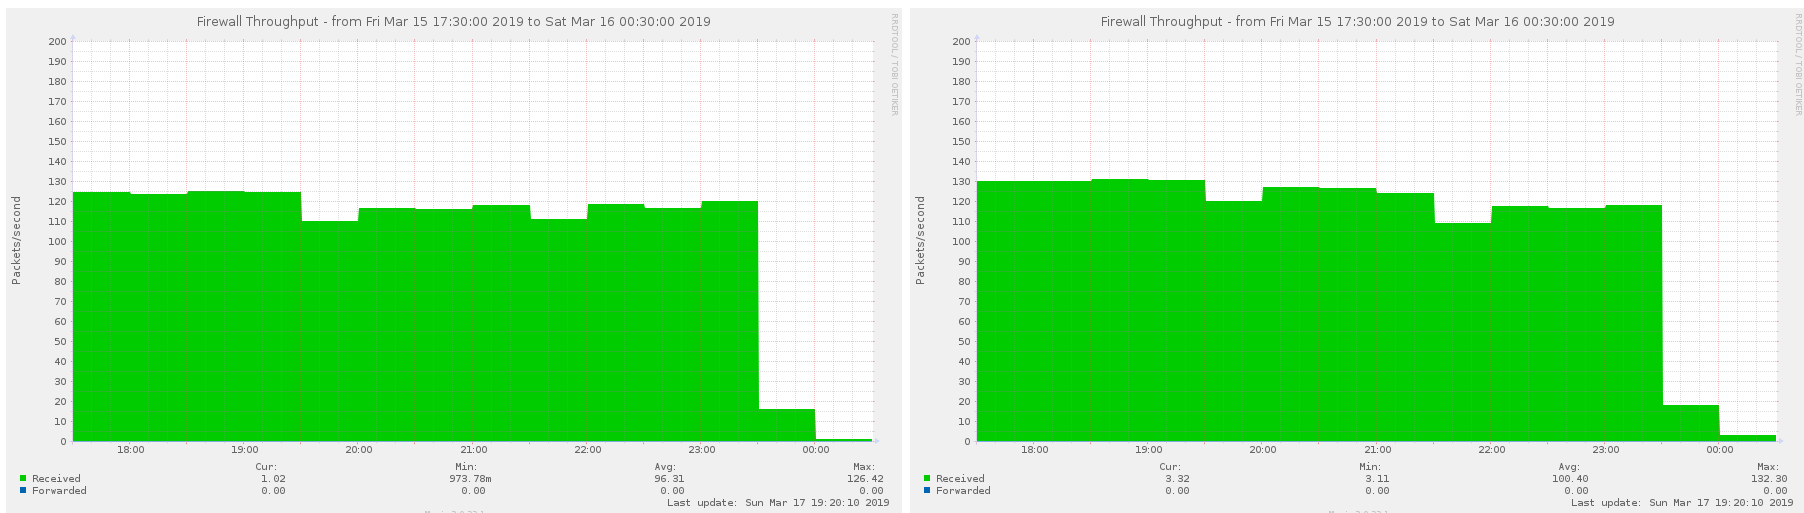
\includegraphics{ResultsAndAnalysis/MopidyServerTestImages/012MopidyFirewallThroughput.png}
\centering
\caption{Mopidy Client and Server Device Firewall Throughput}
\label{MopidyFirewallThroughput}
\end{figure}

\begin{figure}[H]
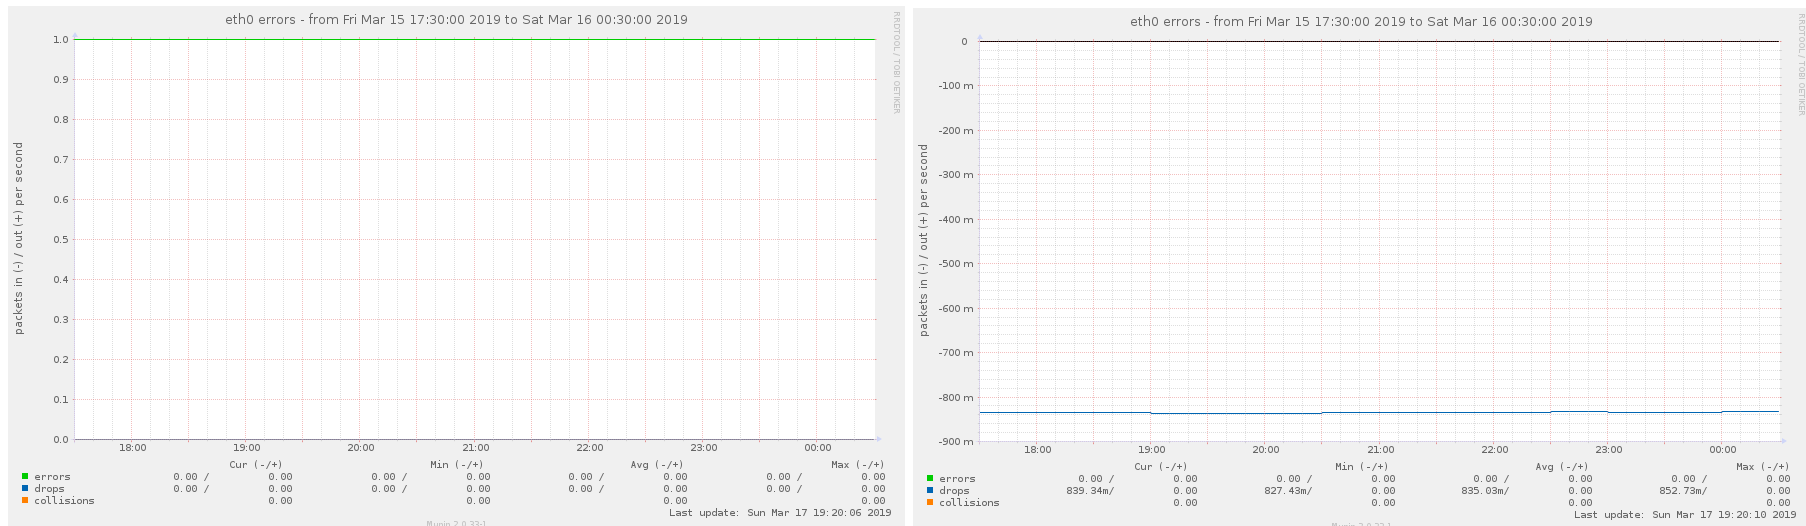
\includegraphics{ResultsAndAnalysis/MopidyServerTestImages/010MopidyEth0Errors.png}
\centering
\caption{Mopidy Client and Server Device Eth Errors}
\label{MopidyEthError}
\end{figure}

\begin{figure}[H]
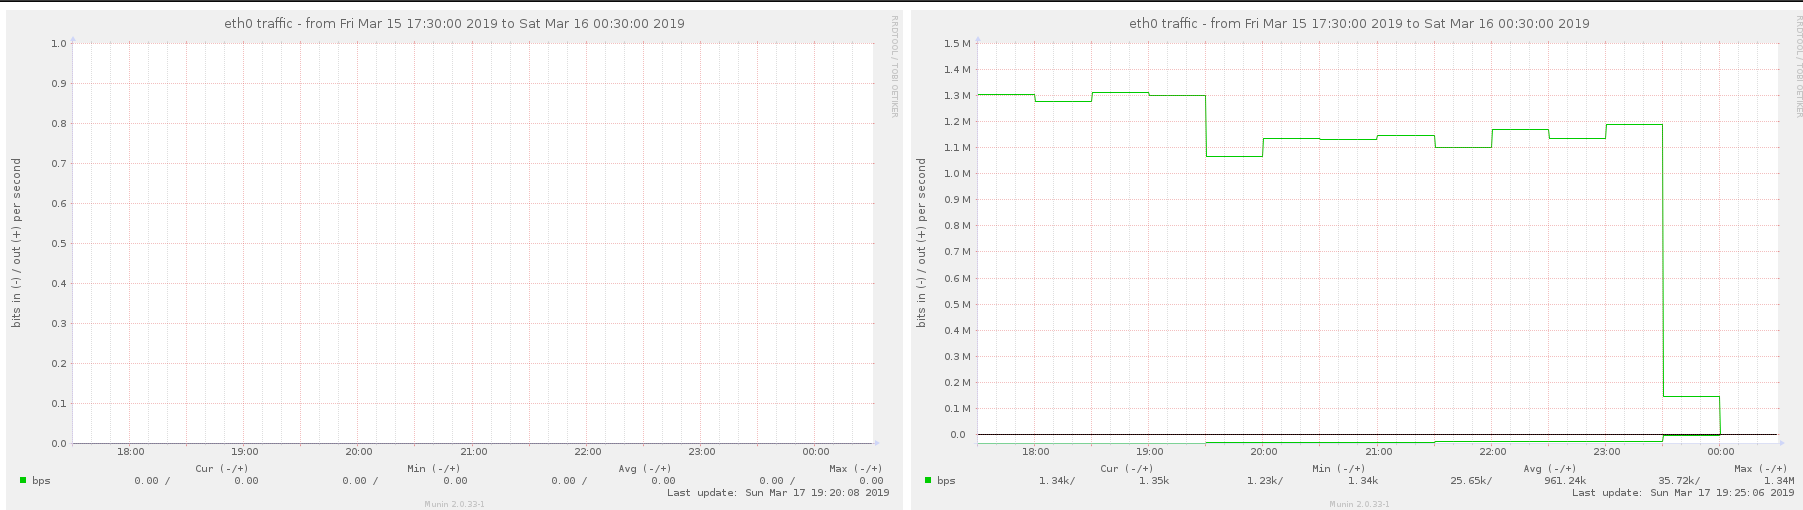
\includegraphics{ResultsAndAnalysis/MopidyServerTestImages/011MopidyEth0Traffic.png}
\centering
\caption{Mopidy Client and Server Device Eth Traffic}
\label{MopidyEthTraffic}
\end{figure}

\begin{figure}[H]
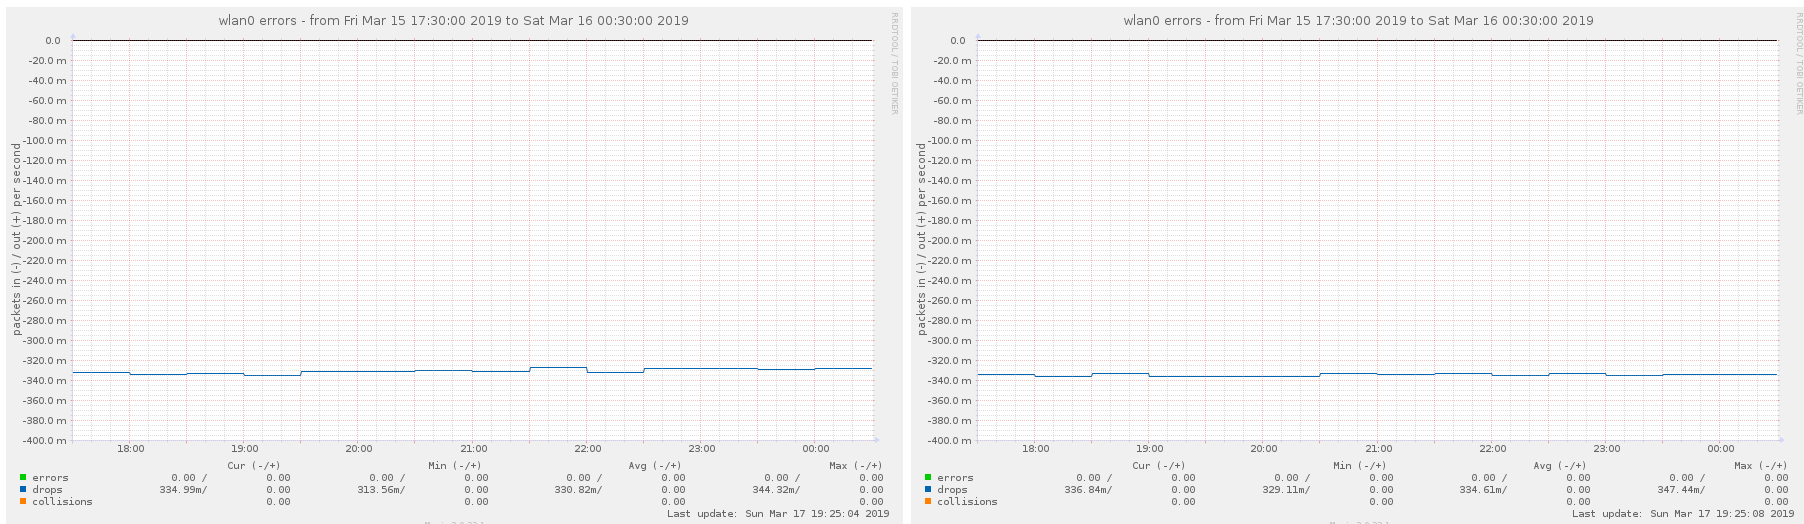
\includegraphics{ResultsAndAnalysis/MopidyServerTestImages/022MopidyWlan0Errors.png}
\centering
\caption{Mopidy Client and Server Device Wlan Errors}
\label{MopidyWlanError}
\end{figure}

\begin{figure}[H]
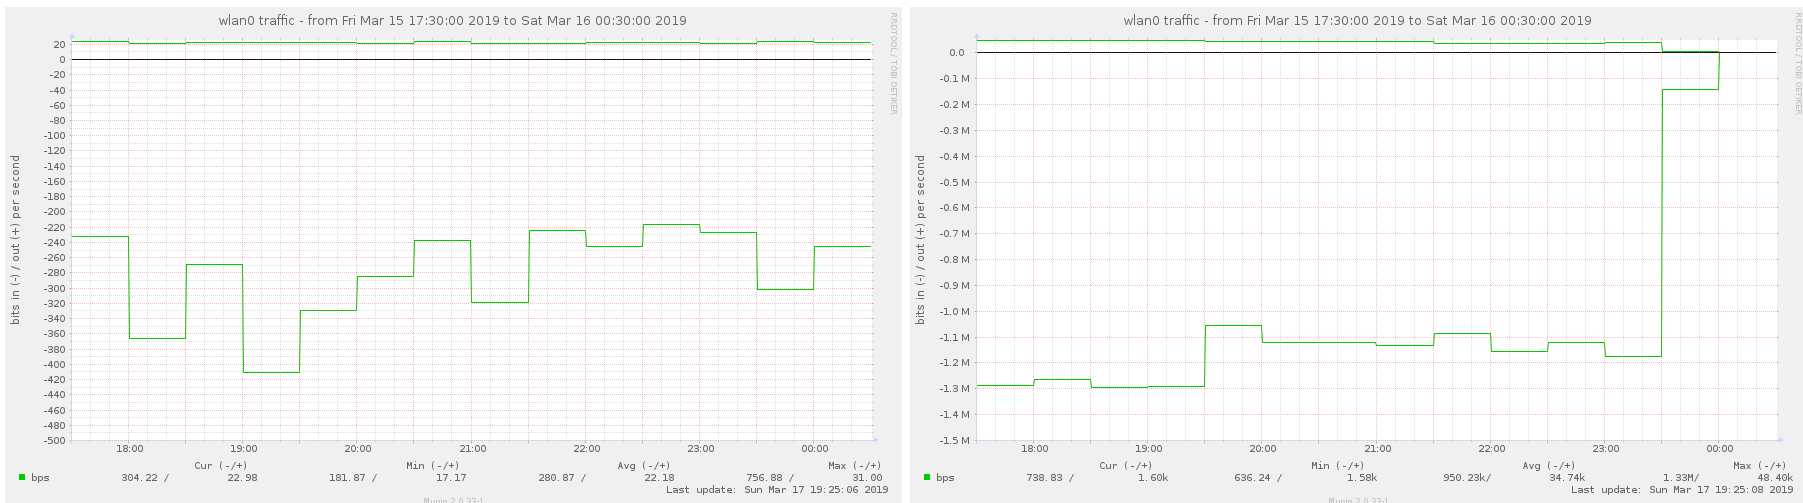
\includegraphics{ResultsAndAnalysis/MopidyServerTestImages/023MopidyWlan0Traffic.png}
\centering
\caption{Mopidy Client and Server Device Wlan Traffic}
\label{MopidyWlanTraffic}
\end{figure}

\begin{figure}[H]
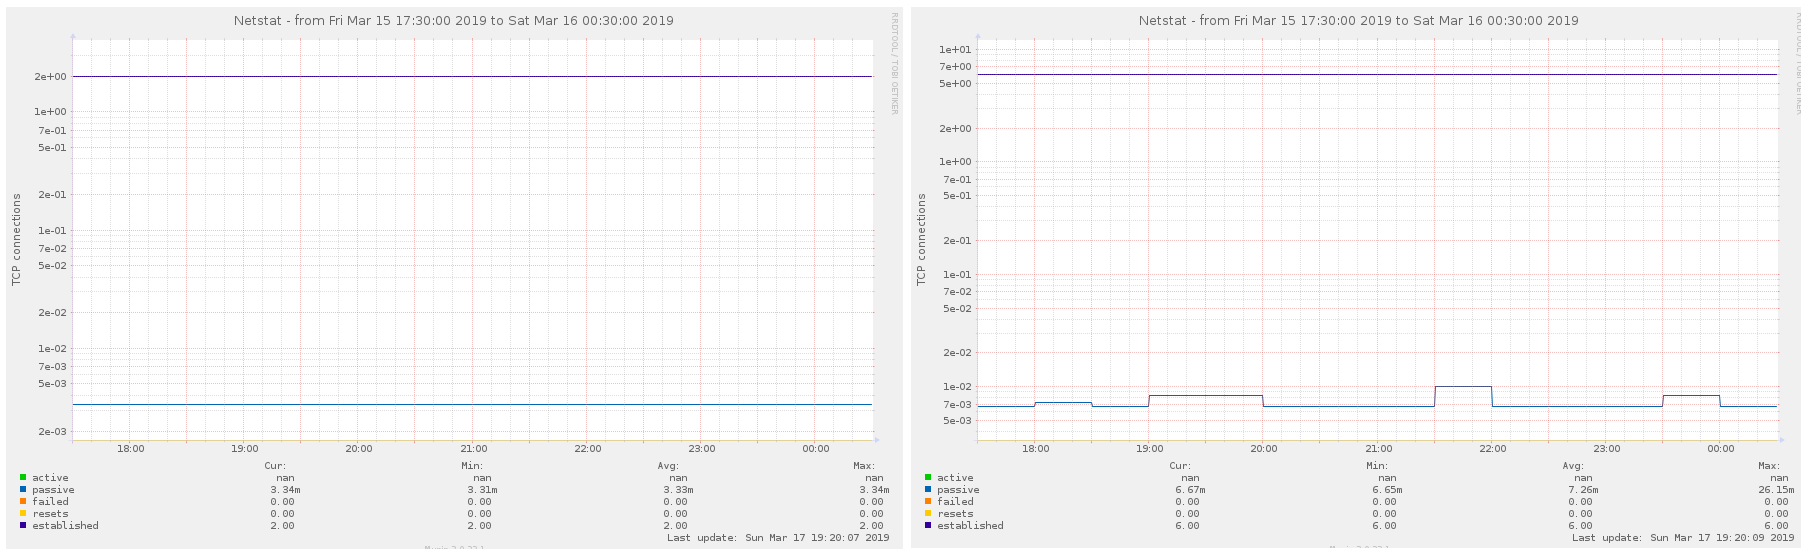
\includegraphics{ResultsAndAnalysis/MopidyServerTestImages/018MopidyNetstat.png}
\centering
\caption{Mopidy Client and Server Device Netstat}
\label{MopidyNetstat}
\end{figure}

\textbf{Processes}

\begin{figure}[H]
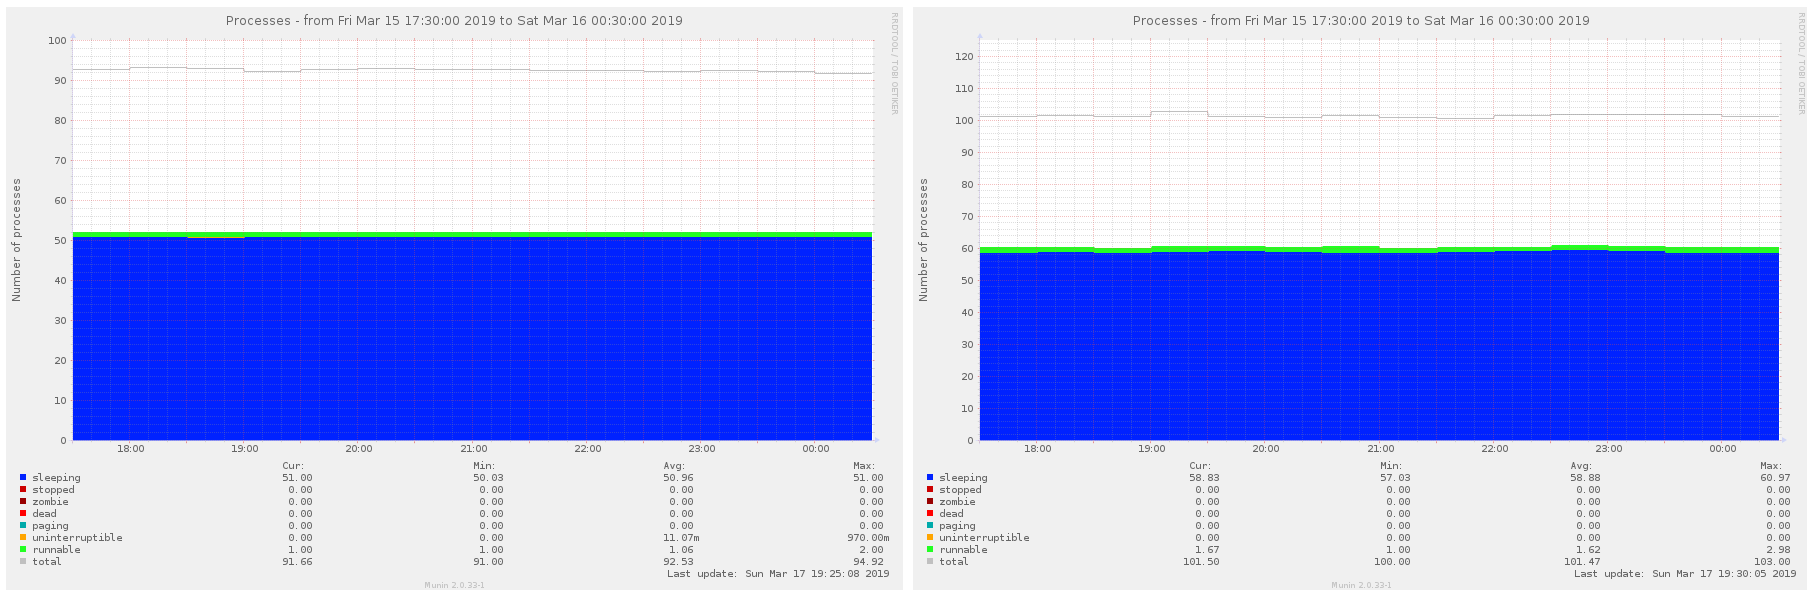
\includegraphics{ResultsAndAnalysis/MopidyServerTestImages/020MopidyProcesses.png}
\centering
\caption{Mopidy Client and Server Device Processes}
\label{MopidyProcesses}
\end{figure}

\begin{figure}[H]
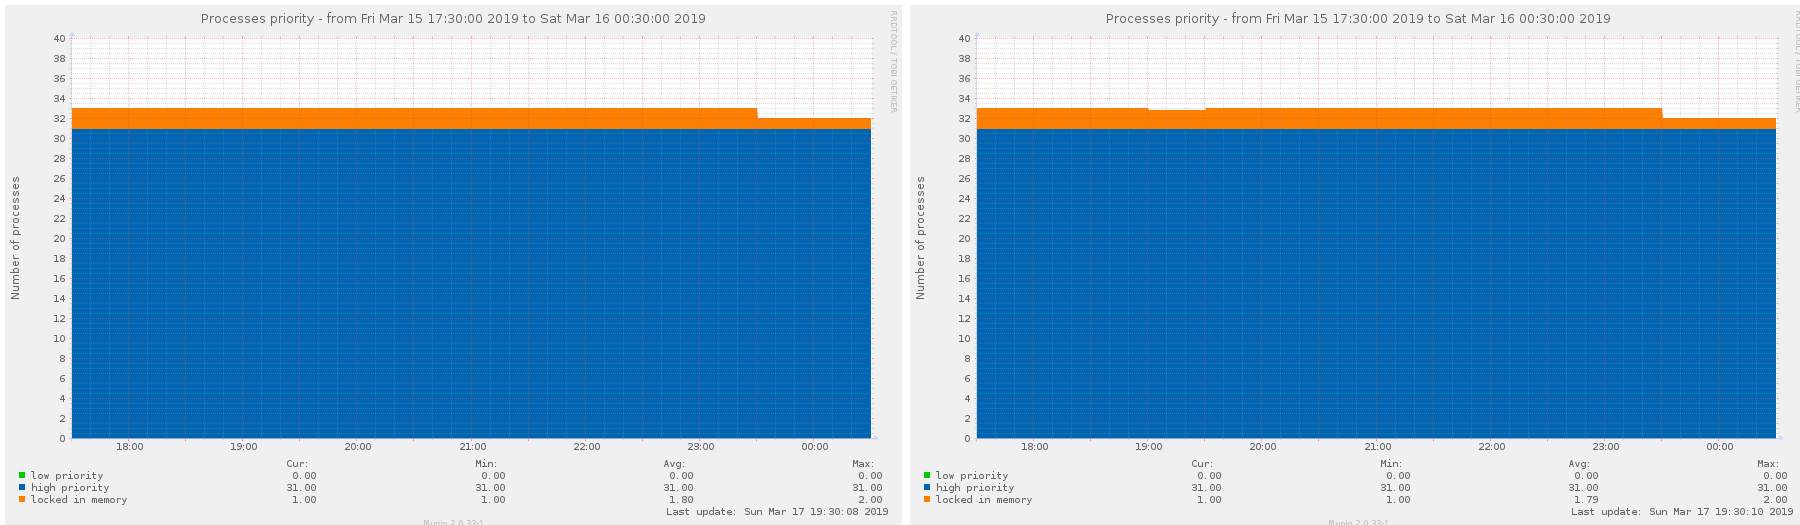
\includegraphics{ResultsAndAnalysis/MopidyServerTestImages/021MopidyProcessPriority.png}
\centering
\caption{Mopidy Client and Server Device Process Priority}
\label{MopidyProcessPriority}
\end{figure}

\begin{figure}[H]
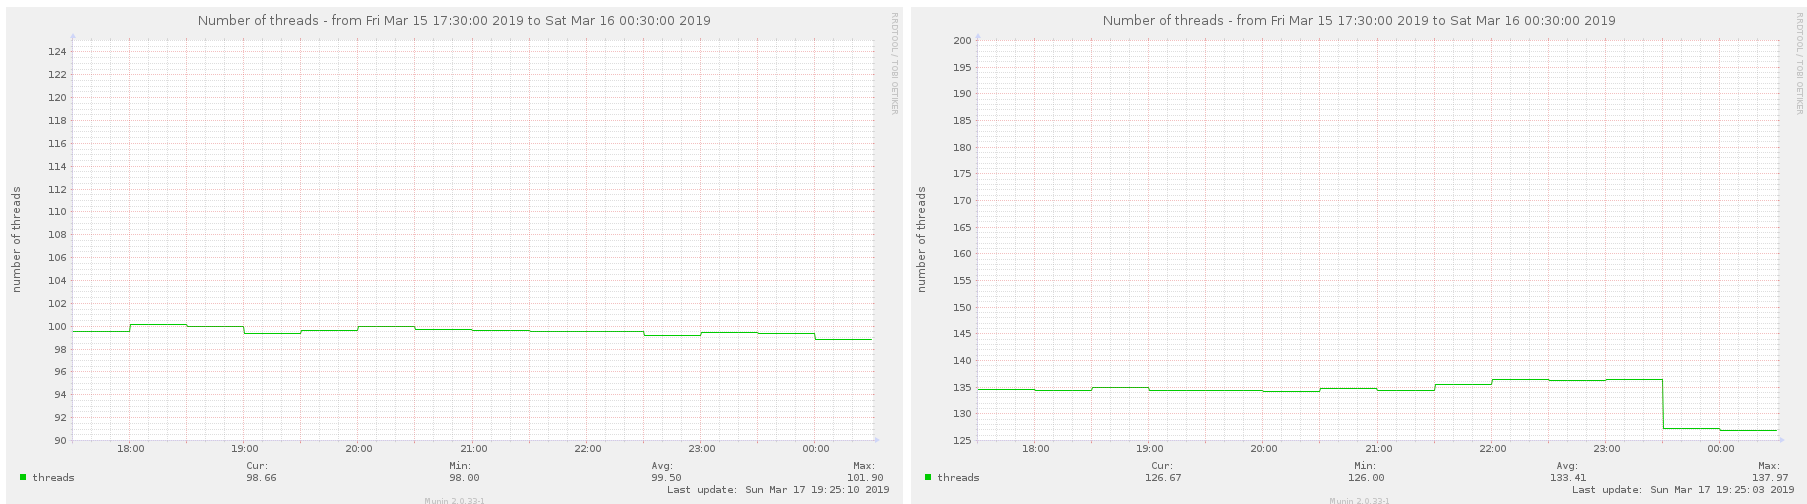
\includegraphics{ResultsAndAnalysis/MopidyServerTestImages/019MopidyNoOfThreads.png}
\centering
\caption{Mopidy Client and Server Device Number of Threads}
\label{MopidyNumThreads}
\end{figure}

\textbf{System}

\begin{figure}[H]
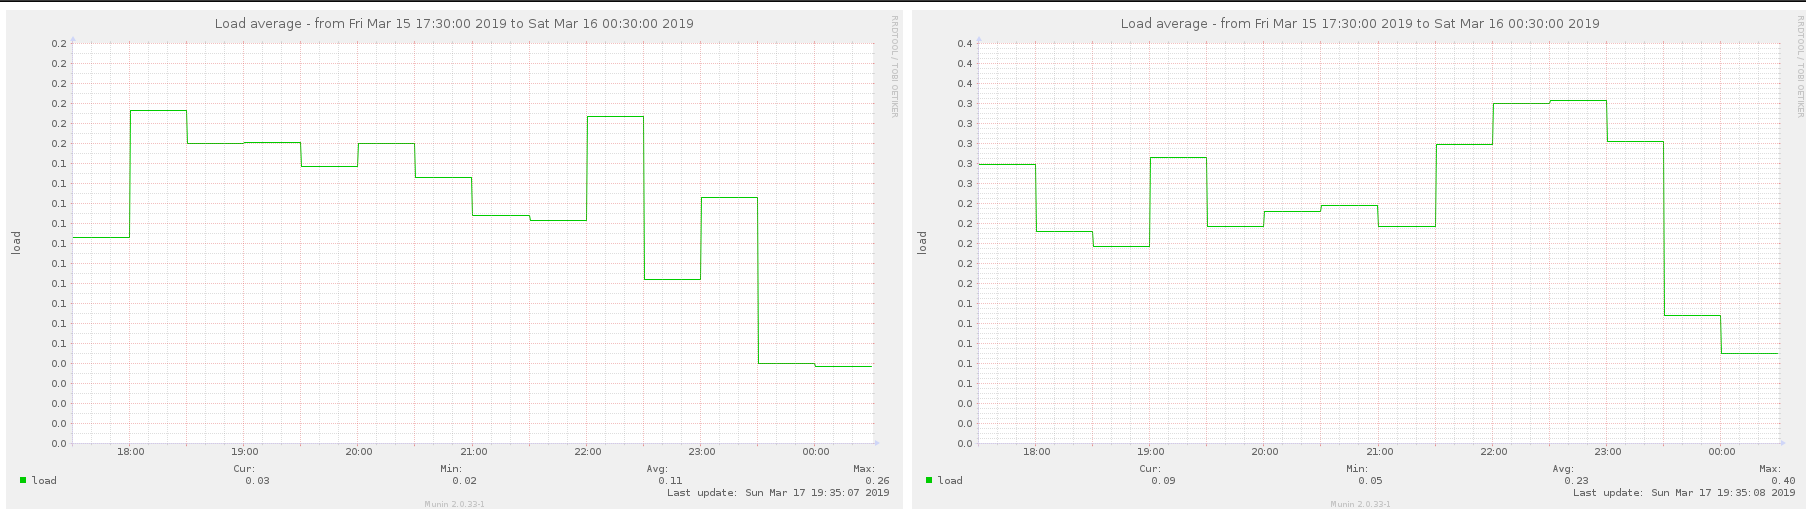
\includegraphics{ResultsAndAnalysis/MopidyServerTestImages/016MopidyLoadAverage.png}
\centering
\caption{Mopidy Client and Server Device Load Average}
\label{MopidyLoadAvg}
\end{figure}

\begin{figure}[H]
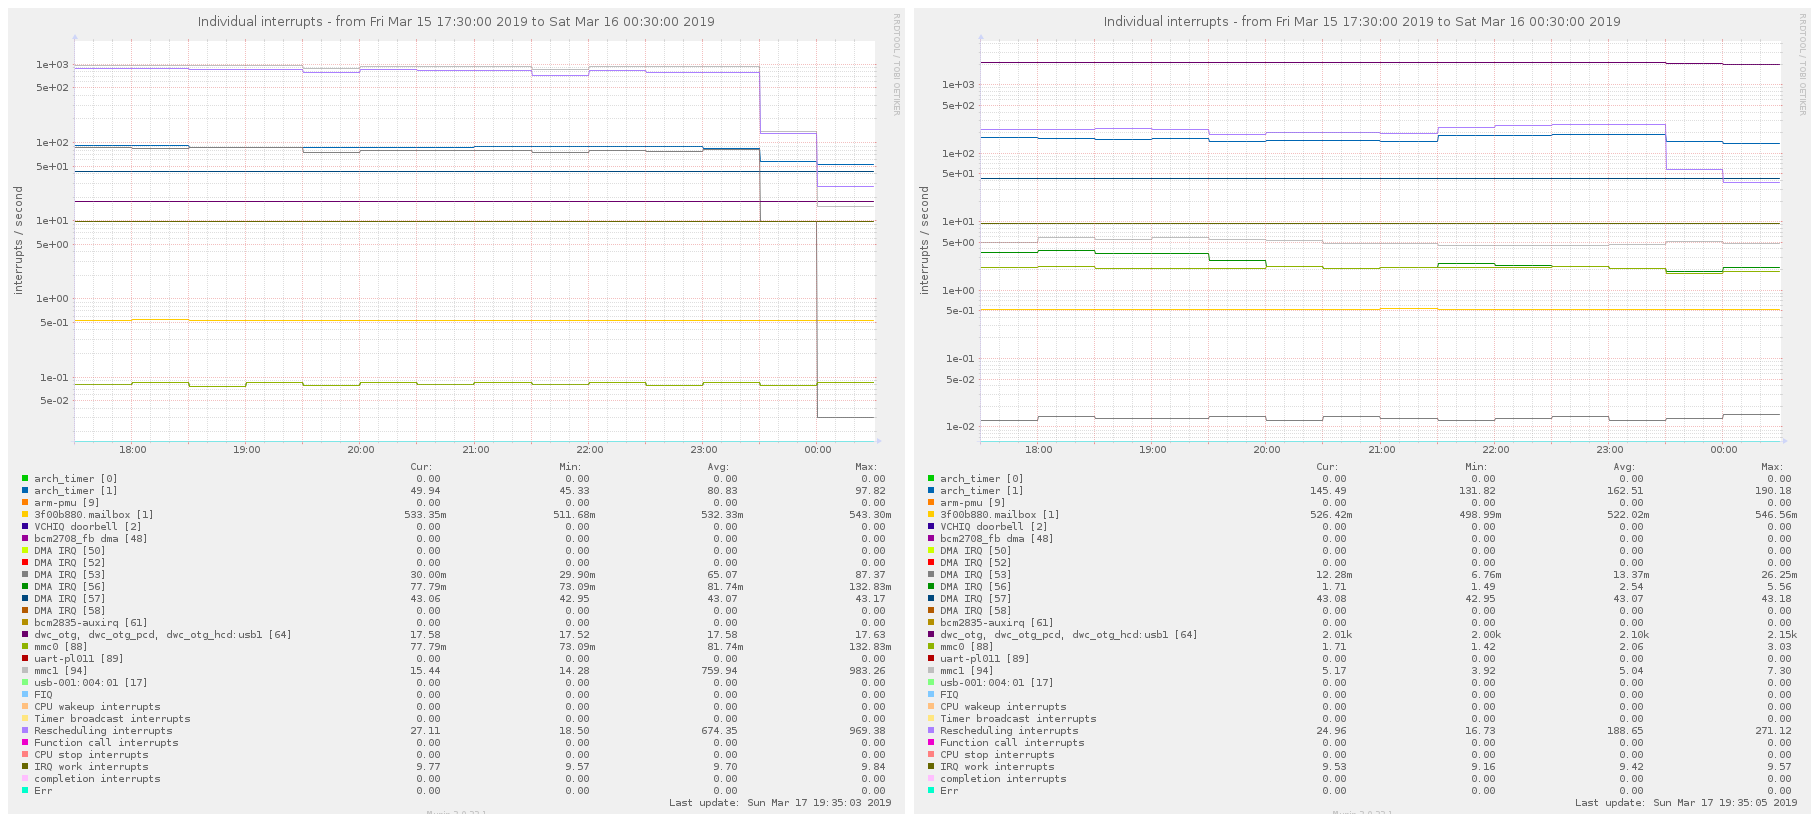
\includegraphics{ResultsAndAnalysis/MopidyServerTestImages/014MopidyIndividualInterrupts.png}
\centering
\caption{Mopidy Client and Server Device Individual Interrupts}
\label{MopidyIndInt}
\end{figure}

\begin{figure}[H]
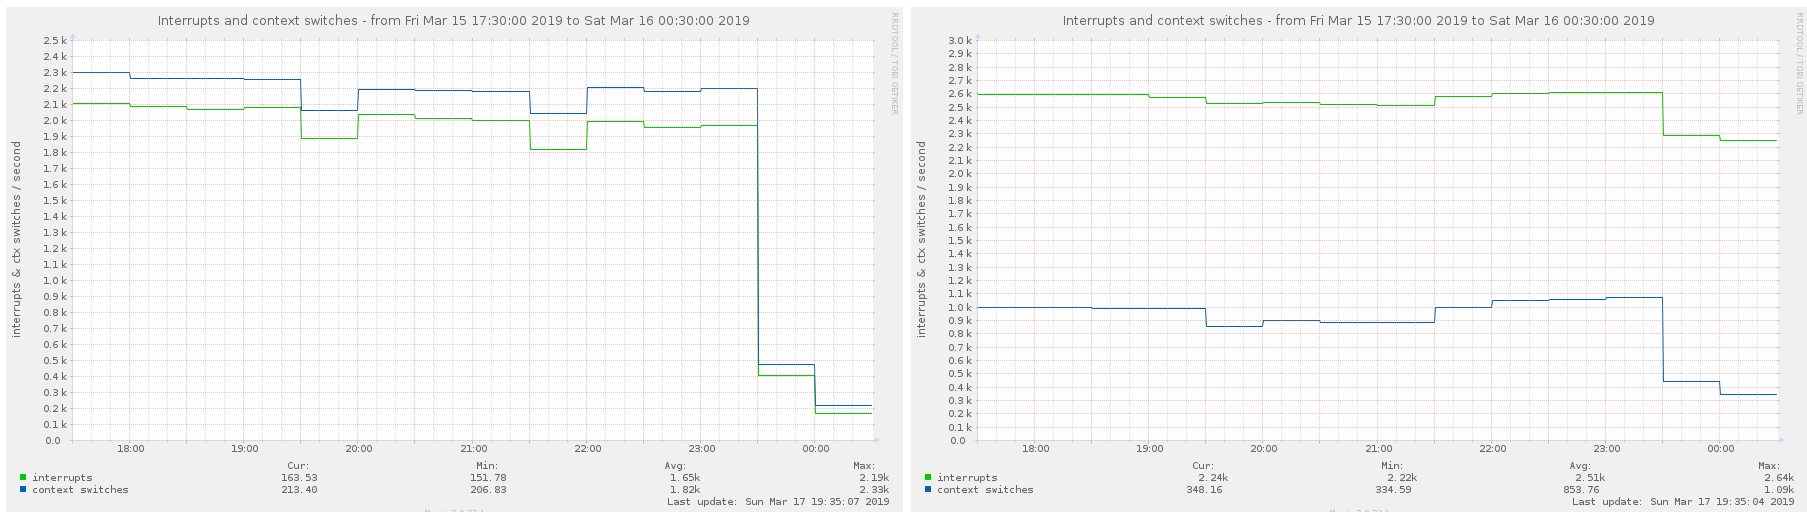
\includegraphics{ResultsAndAnalysis/MopidyServerTestImages/015MopidyInterruptsAndContextSwitches.png}
\centering
\caption{Mopidy Client and Server Device Interrupts and Context Switches}
\label{MopidyIntCont}
\end{figure}

\begin{figure}[H]
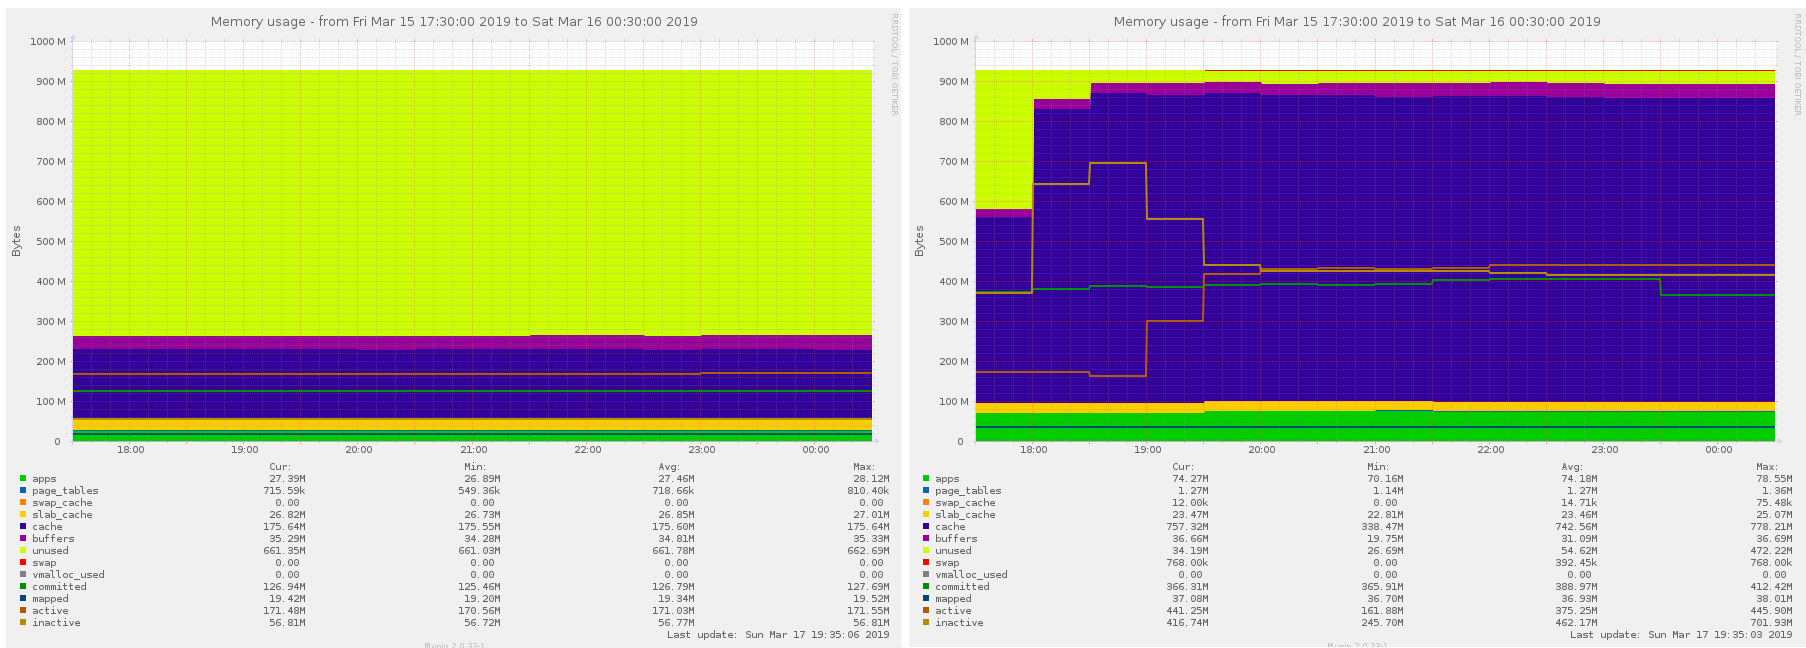
\includegraphics{ResultsAndAnalysis/MopidyServerTestImages/017MopidyMemoryUsage.png}
\centering
\caption{Mopidy Client and Server Device Memory Usage}
\label{MopidyMemUse}
\end{figure}

\begin{figure}[H]
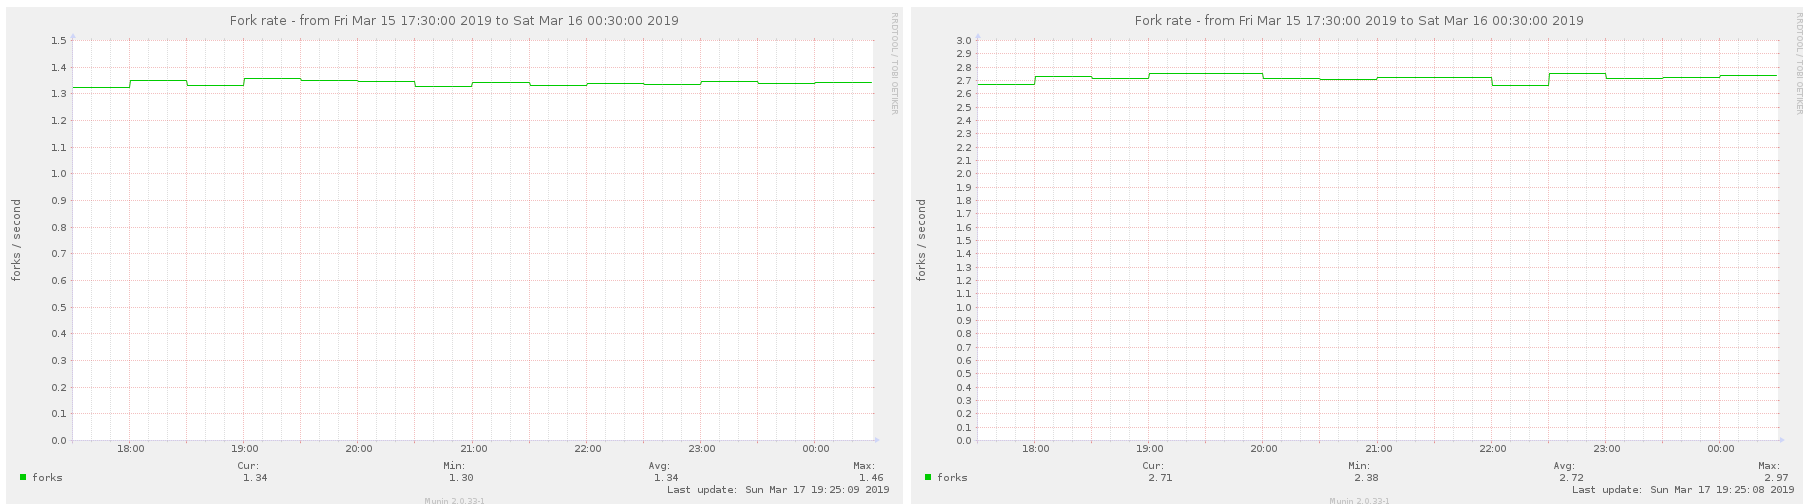
\includegraphics{ResultsAndAnalysis/MopidyServerTestImages/013MopidyForkRate.png}
\centering
\caption{Mopidy Client and Server Device Fork Rate}
\label{MopidyForkRate}
\end{figure}

\begin{figure}[H]
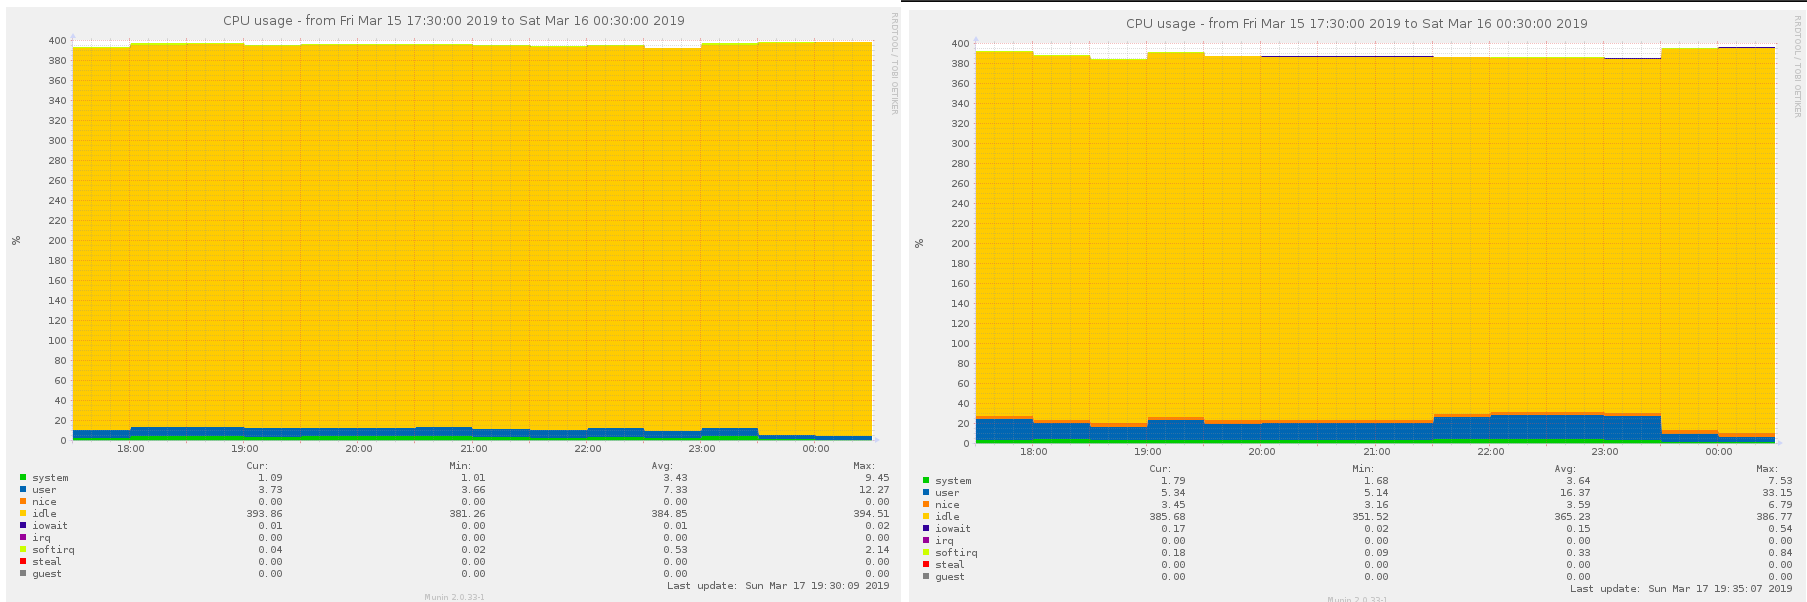
\includegraphics{ResultsAndAnalysis/MopidyServerTestImages/004MopidyCPUUsage.png}
\centering
\caption{Mopidy Client and Server Device CPU Usage}
\label{MopidyCPUUsage}
\end{figure}

\textbf{Sensors}

\begin{figure}[H]
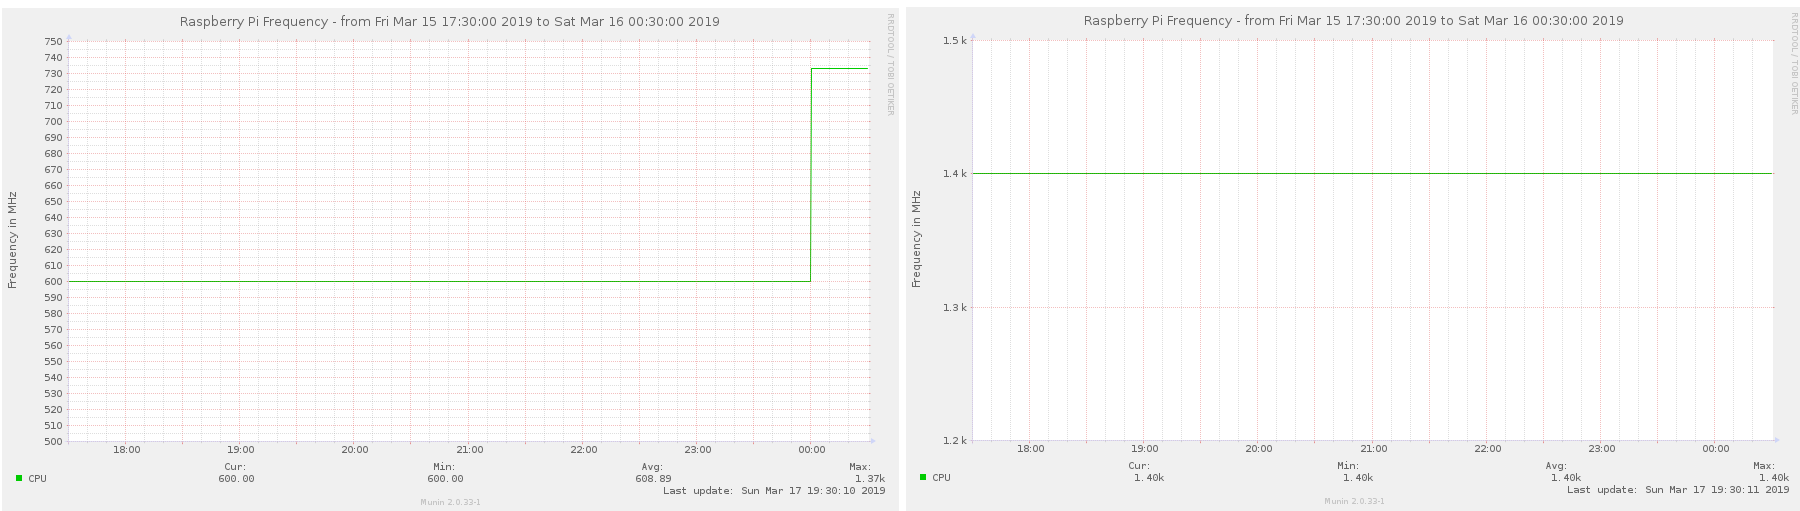
\includegraphics{ResultsAndAnalysis/MopidyServerTestImages/001MopidyCPUFreq.png}
\centering
\caption{Mopidy Client and Server Device CPU Frequency}
\label{MopidyCPUFreq}
\end{figure}

\begin{figure}[H]
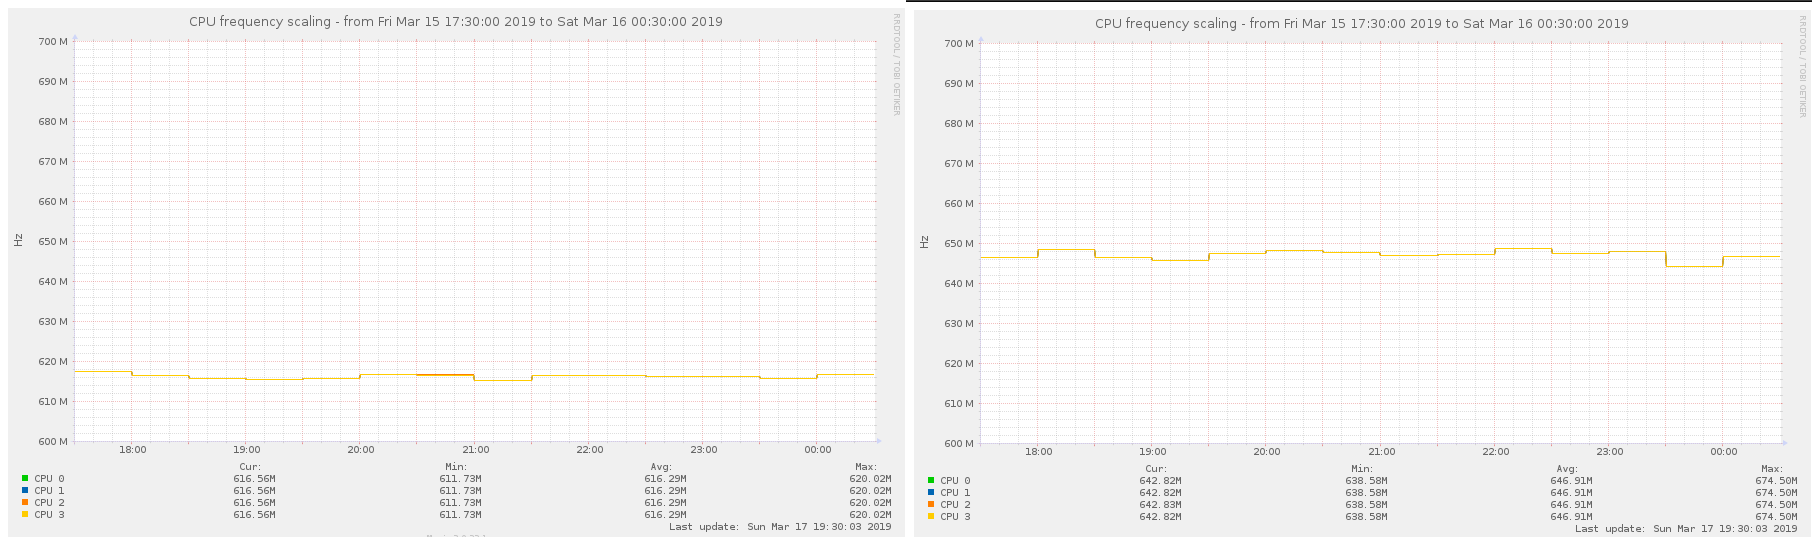
\includegraphics{ResultsAndAnalysis/MopidyServerTestImages/002MopidyCPUFreqScaling.png}
\centering
\caption{Mopidy Client and Server Device CPU Frequency Scaling}
\label{MopidyCPUFreqScaling}
\end{figure}

\begin{figure}[H]
\includegraphics{ResultsAndAnalysis/MopidyServerTestImages/003MopidyCPUTemp.png}
\centering
\caption{Mopidy Client and Server Device CPU Temperature}
\label{MopidyCPUTemp}
\end{figure}

\subsection{Volumio}\label{volumio-2}

\textbf{Disk}

\begin{figure}[H]
\includegraphics{ResultsAndAnalysis/VolumioServerTestImages/005VolumioDiskIO.png}
\centering
\caption{Volumio Disk I/O on Client and Server Device}
\label{VolumioDiskIO}
\end{figure}

\begin{figure}[H]
\includegraphics{ResultsAndAnalysis/VolumioServerTestImages/006VolumioDiskLatency.png}
\centering
\caption{Volumio Client and Server Device Disk Latency}
\label{VolumioDiskLatency}
\end{figure}

\begin{figure}[H]
\includegraphics{ResultsAndAnalysis/VolumioServerTestImages/007VolumioDiskThroughput.png}
\centering
\caption{Volumio Client and Server Device Disk Throughput}
\label{VolumioDiskThroughput}
\end{figure}

\begin{figure}[H]
\includegraphics{ResultsAndAnalysis/VolumioServerTestImages/009VolumioDiskUtilization.png}
\centering
\caption{Volumio Client and Server Device Disk Utilization}
\label{VolumioDiskUtil}
\end{figure}

\textbf{Network}

\begin{figure}[H]
\includegraphics{ResultsAndAnalysis/VolumioServerTestImages/012VolumioFirewallThroughput.png}
\centering
\caption{Volumio Client and Server Device Firewall Throughput}
\label{VolumioFirewallThroughput}
\end{figure}

\begin{figure}[H]
\includegraphics{ResultsAndAnalysis/VolumioServerTestImages/010VolumioEth0Errors.png}
\centering
\caption{Volumio Client and Server Device Eth Errors}
\label{VolumioEthError}
\end{figure}

\begin{figure}[H]
\includegraphics{ResultsAndAnalysis/VolumioServerTestImages/011VolumioEth0Traffic.png}
\centering
\caption{Volumio Client and Server Device Eth Traffic}
\label{VolumioEthTraffic}
\end{figure}

\begin{figure}[H]
\includegraphics{ResultsAndAnalysis/VolumioServerTestImages/022VolumioWlan0Errors.png}
\centering
\caption{Volumio Client and Server Device Wlan Errors}
\label{VolumioWlanError}
\end{figure}

\begin{figure}[H]
\includegraphics{ResultsAndAnalysis/VolumioServerTestImages/023VolumioWlan0Traffic.png}
\centering
\caption{Volumio Client and Server Device Wlan Traffic}
\label{VolumioWlanTraffic}
\end{figure}

\begin{figure}[H]
\includegraphics{ResultsAndAnalysis/VolumioServerTestImages/018VolumioNetstat.png}
\centering
\caption{Volumio Client and Server Device Netstat}
\label{VolumioNetstat}
\end{figure}

\textbf{Processes}

\begin{figure}[H]
\includegraphics{ResultsAndAnalysis/VolumioServerTestImages/020VolumioProcesses.png}
\centering
\caption{Volumio Client and Server Device Processes}
\label{VolumioProcesses}
\end{figure}

\begin{figure}[H]
\includegraphics{ResultsAndAnalysis/VolumioServerTestImages/021VolumioProcessPriority.png}
\centering
\caption{Volumio Client and Server Device Processes}
\label{VolumioProcessPriority}
\end{figure}

\begin{figure}[H]
\includegraphics{ResultsAndAnalysis/VolumioServerTestImages/019VolumioNoOfThreads.png}
\centering
\caption{Volumio Client and Server Device Number of Threads}
\label{VolumioNumThreads}
\end{figure}

\textbf{System}

\begin{figure}[H]
\includegraphics{ResultsAndAnalysis/VolumioServerTestImages/016VolumioLoadAverage.png}
\centering
\caption{Volumio Client and Server Device Load Average}
\label{VolumioLoadAvg}
\end{figure}

\begin{figure}[H]
\includegraphics{ResultsAndAnalysis/VolumioServerTestImages/014VolumioIndividualInterrupts.png}
\centering
\caption{Volumio Client and Server Device Individual Interrupts}
\label{VolumioIndInt}
\end{figure}

\begin{figure}[H]
\includegraphics{ResultsAndAnalysis/VolumioServerTestImages/015VolumioInterruptsAndContextSwitches.png}
\centering
\caption{Volumio Client and Server Device Interrupts and Context Switches}
\label{VolumioIntCont}
\end{figure}

\begin{figure}[H]
\includegraphics{ResultsAndAnalysis/VolumioServerTestImages/017VolumioMemoryUsage.png}
\centering
\caption{Volumio Client and Server Device Memory Usage}
\label{VolumioMemUse}
\end{figure}

\begin{figure}[H]
\includegraphics{ResultsAndAnalysis/VolumioServerTestImages/013VolumioForkRate.png}
\centering
\caption{Volumio Client and Server Device Fork Rate}
\label{VolumioForkRate}
\end{figure}

\begin{figure}[H]
\includegraphics{ResultsAndAnalysis/VolumioServerTestImages/004VolumioCPUUsage.png}
\centering
\caption{Volumio Client and Server Device CPU Usage}
\label{VolumioCPUUsage}
\end{figure}

\textbf{Sensors}

\begin{figure}[H]
\includegraphics{ResultsAndAnalysis/VolumioServerTestImages/001VolumioCPUFreq.png}
\centering
\caption{Volumio Client and Server Device CPU Frequency}
\label{VolumioCPUFreq}
\end{figure}

\begin{figure}[H]
\includegraphics{ResultsAndAnalysis/VolumioServerTestImages/002VolumioCPUFreqScaling.png}
\centering
\caption{Volumio Client and Server Device CPU Frequency Scaling}
\label{VolumioCPUFreqScaling}
\end{figure}

\begin{figure}[H]
\includegraphics{ResultsAndAnalysis/VolumioServerTestImages/003VolumioCPUTemp.png}
\centering
\caption{Volumio Client and Server Device CPU Temperature}
\label{VolumioCPUTemp}
\end{figure}

\section{\texorpdfstring{Audio Server Software Munin Data Tables
\label{AppendicesAudioServerSoftwareTables}}{Audio Server Software Munin Data Tables }}\label{audio-server-software-munin-data-tables}

\subsection{MPD}\label{mpd-3}

\begin{table}[H]
\centering
    \begin{tabular}{||c|c|c|c|c|c|c||}
    \hline
    \multicolumn{7}{|c|}{\textbf{Disk (Client)}} \\
    \hline
    \multicolumn{7}{|c|}{\textbf{Disk I/O}} \\
    \hline\hline
      & \multicolumn{2}{|c|}{Min} & \multicolumn{2}{|c|}{Avg} & \multicolumn{2}{|c|}{Max} \\
    \hline
      & - & + & - & + & - & + \\
    \hline
    IO/sec & 0.00 & 66.79m & 0.00 & 82.31m & 0.00 & 141.08m \\
    \hline
    Req Size (KB) & 0.00 & 6.66 & 0.00 & 8.46 & 0.00 & 10.30 \\
    \hline\hline
    \multicolumn{7}{|c|}{\textbf{Disk Latency}} \\
    \hline\hline
      & \multicolumn{2}{|c|}{Min} & \multicolumn{2}{|c|}{Avg} & \multicolumn{2}{|c|}{Max} \\
    \hline
    Device I/O Time  & \multicolumn{2}{|c|}{926.77u} & \multicolumn{2}{|c|}{1.60m} & \multicolumn{2}{|c|}{2.58m} \\
    \hline
    I/O Wait Time  & \multicolumn{2}{|c|}{4.20} & \multicolumn{2}{|c|}{7.32m} & \multicolumn{2}{|c|}{16.60m} \\
    \hline
    Read I/O Time  & \multicolumn{2}{|c|}{0.00m} & \multicolumn{2}{|c|}{0.00m} & \multicolumn{2}{|c|}{0.00m} \\
    \hline
    Write I/O Time  & \multicolumn{2}{|c|}{4.20m} & \multicolumn{2}{|c|}{7.32m} & \multicolumn{2}{|c|}{16.60m} \\
    \hline\hline
    \multicolumn{7}{|c|}{\textbf{Disk Throughput}} \\
    \hline\hline
      & \multicolumn{2}{|c|}{Min} & \multicolumn{2}{|c|}{Avg} & \multicolumn{2}{|c|}{Max} \\
    \hline
      & - & + & - & + & - & + \\
    \hline
    Bytes & 0.00 & 453.23 & 0.00 & 697.68 & 0.00 & 1.23k \\
    \hline\hline
    \multicolumn{7}{|c|}{\textbf{Disk Utilization}} \\
    \hline\hline
      & \multicolumn{2}{|c|}{Min} & \multicolumn{2}{|c|}{Avg} & \multicolumn{2}{|c|}{Max} \\
    \hline
    Utilization (\%Busy)  & \multicolumn{2}{|c|}{0.01} & \multicolumn{2}{|c|}{0.01} & \multicolumn{2}{|c|}{0.02} \\
    \hline\hline
    \end{tabular}
    \caption{MPD SnapClient Device Disk Parameters}
    \label{MPDclientDiskTab}
\end{table}

\begin{table}[H]
\centering
    \begin{tabular}{||c|c|c|c|c|c|c||}
    \hline
    \multicolumn{7}{|c|}{\textbf{Disk (Server)}} \\
    \hline
    \multicolumn{7}{|c|}{\textbf{Disk I/O}} \\
    \hline\hline
      & \multicolumn{2}{|c|}{Min} & \multicolumn{2}{|c|}{Avg} & \multicolumn{2}{|c|}{Max} \\
    \hline
      & - & + & - & + & - & + \\
    \hline
    IO/sec & 0.00 & 69.87m & 252.42m & 422.49m & 1.03 & 536.13m \\
    \hline
    Req Size (KB) & 0.00 & 6.40 & 113.98 & 6.98 & 296.23 & 8.55 \\
    \hline\hline
    \multicolumn{7}{|c|}{\textbf{Disk Latency}} \\
    \hline\hline
      & \multicolumn{2}{|c|}{Min} & \multicolumn{2}{|c|}{Avg} & \multicolumn{2}{|c|}{Max} \\
    \hline
    Device I/O Time  & \multicolumn{2}{|c|}{397.44u} & \multicolumn{2}{|c|}{43.4m} & \multicolumn{2}{|c|}{10.33m} \\
    \hline
    I/O Wait Time  & \multicolumn{2}{|c|}{1.18m} & \multicolumn{2}{|c|}{6.21m} & \multicolumn{2}{|c|}{15.21m} \\
    \hline
    Read I/O Time  & \multicolumn{2}{|c|}{0.00m} & \multicolumn{2}{|c|}{7.65m} & \multicolumn{2}{|c|}{20.36m} \\
    \hline
    Write I/O Time  & \multicolumn{2}{|c|}{1.18m} & \multicolumn{2}{|c|}{3.00m} & \multicolumn{2}{|c|}{9.56m} \\
    \hline\hline
    \multicolumn{7}{|c|}{\textbf{Disk Throughput}} \\
    \hline\hline
      & \multicolumn{2}{|c|}{Min} & \multicolumn{2}{|c|}{Avg} & \multicolumn{2}{|c|}{Max} \\
    \hline
      & - & + & - & + & - & + \\
    \hline
    Bytes & 0.00 & 572.00 & 59.27k & 2.82k & 185.35k & 3.94k \\
    \hline\hline
    \multicolumn{7}{|c|}{\textbf{Disk Utilization}} \\
    \hline\hline
      & \multicolumn{2}{|c|}{Min} & \multicolumn{2}{|c|}{Avg} & \multicolumn{2}{|c|}{Max} \\
    \hline
    Utilization (\%Busy)  & \multicolumn{2}{|c|}{0.00} & \multicolumn{2}{|c|}{0.39} & \multicolumn{2}{|c|}{1.17} \\
    \hline\hline
    \end{tabular}
    \caption{MPD Server Device Disk Parameters}
    \label{MPDserverDiskTab}
\end{table}

\begin{table}[H]
\centering
    \begin{tabular}{||c|c|c|c|c|c|c||}
    \hline
    \multicolumn{7}{|c|}{\textbf{Network (Client)}} \\
    \hline
    \multicolumn{7}{|c|}{\textbf{Firewall Throughput (Packets/sec}} \\
    \hline\hline
      & \multicolumn{2}{|c|}{Min} & \multicolumn{2}{|c|}{Avg} & \multicolumn{2}{|c|}{Max} \\
    \hline\hline
      & - & + & - & + & - & + \\
    \hline
    Received & \multicolumn{2}{|c|}{983.67m} & \multicolumn{2}{|c|}{99.33} & \multicolumn{2}{|c|}{126.69} \\
    \hline
    Forwarded & \multicolumn{2}{|c|}{0.00} & \multicolumn{2}{|c|}{0.00} & \multicolumn{2}{|c|}{0.00} \\
    \hline\hline
    \multicolumn{7}{|c|}{\textbf{Eth0 Errors}} \\
    \hline\hline
      & \multicolumn{2}{|c|}{Min} & \multicolumn{2}{|c|}{Avg} & \multicolumn{2}{|c|}{Max} \\
    \hline
     & - & + & - & + & - & + \\
    \hline
    Errors & 0.00 & 0.00 & 0.00 & 0.00 & 0.00 & 0.00 \\
    \hline
    Drops & 0.00 & 0.00 & 0.00 & 0.00 & 0.00 & 0.00 \\
    \hline
    Collisions & 0.00 & 0.00 & 0.00 & 0.00 & 0.00 & 0.00 \\
    \hline\hline
    \multicolumn{7}{|c|}{\textbf{Eth0 Traffic}} \\
    \hline\hline
      & \multicolumn{2}{|c|}{Min} & \multicolumn{2}{|c|}{Avg} & \multicolumn{2}{|c|}{Max} \\
    \hline
      & - & + & - & + & - & + \\
    \hline
    bps & 0.00 & 0.00 & 0.00 & 0.00 & 0.00 & 0.00 \\
    \hline\hline
    \multicolumn{7}{|c|}{\textbf{Wlan0 Errors}} \\
    \hline\hline
      & \multicolumn{2}{|c|}{Min} & \multicolumn{2}{|c|}{Avg} & \multicolumn{2}{|c|}{Max} \\
    \hline
      & - & + & - & + & - & + \\
    \hline
    Errors  & 0.00 & 0.00 & 0.00 & 0.00 & 0.00 & 0.00 \\
    \hline
    Drops & 270.53m & 0.00 & 302.72m & 0.00 & 343.80m & 0.00 \\
    \hline
    Collisions & \multicolumn{2}{|c|}{0.00} & \multicolumn{2}{|c|}{0.00} & \multicolumn{2}{|c|}{0.00} \\
    \hline\hline
    \multicolumn{7}{|c|}{\textbf{Wlan0 Traffic}} \\
    \hline\hline
      & \multicolumn{2}{|c|}{Min} & \multicolumn{2}{|c|}{Avg} & \multicolumn{2}{|c|}{Max} \\
    \hline
      & - & + & - & + & - & + \\
    \hline
    bps  & 669.92 & 1.58k & 939.62k & 31.80k & 1.26M & 39.03k \\
    \hline\hline
    \multicolumn{7}{|c|}{\textbf{Netstat (TCP Connections)}} \\
    \hline\hline
      & \multicolumn{2}{|c|}{Min} & \multicolumn{2}{|c|}{Avg} & \multicolumn{2}{|c|}{Max} \\
    \hline
    active & \multicolumn{2}{|c|}{nan} & \multicolumn{2}{|c|}{nan} & \multicolumn{2}{|c|}{nan} \\
    \hline
    passive & \multicolumn{2}{|c|}{3.31m} & \multicolumn{2}{|c|}{3.33m} & \multicolumn{2}{|c|}{3.35m} \\
    \hline
    failed & \multicolumn{2}{|c|}{0.00} & \multicolumn{2}{|c|}{0.00} & \multicolumn{2}{|c|}{0.00} \\
    \hline
    resets & \multicolumn{2}{|c|}{0.00} & \multicolumn{2}{|c|}{39.22u} & \multicolumn{2}{|c|}{3.26m} \\
    \hline
    established & \multicolumn{2}{|c|}{2.00} & \multicolumn{2}{|c|}{2.26} & \multicolumn{2}{|c|}{3.00} \\
    \hline\hline
    \end{tabular}
    \caption{MPD SnapClient Device Network Parameters}
    \label{MPDclientNetTab}
\end{table}

\begin{table}[H]
\centering
    \begin{tabular}{||c|c|c|c|c|c|c||}
    \hline
    \multicolumn{7}{|c|}{\textbf{Network (Server)}} \\
    \hline
    \multicolumn{7}{|c|}{\textbf{Firewall Throughput (Packets/sec}} \\
    \hline\hline
      & \multicolumn{2}{|c|}{Min} & \multicolumn{2}{|c|}{Avg} & \multicolumn{2}{|c|}{Max} \\
    \hline
      & - & + & - & + & - & + \\
    \hline
    Received & \multicolumn{2}{|c|}{1.91} & \multicolumn{2}{|c|}{99.26} & \multicolumn{2}{|c|}{122.94} \\
    \hline
    Forwarded & \multicolumn{2}{|c|}{0.00} & \multicolumn{2}{|c|}{0.00} & \multicolumn{2}{|c|}{0.00} \\
    \hline\hline
    \multicolumn{7}{|c|}{\textbf{Eth0 Errors}} \\
    \hline\hline
      & \multicolumn{2}{|c|}{Min} & \multicolumn{2}{|c|}{Avg} & \multicolumn{2}{|c|}{Max} \\
    \hline
     & - & + & - & + & - & + \\
    \hline
    Errors & 0.00 & 0.00 & 0.00 & 0.00 & 0.00 & 0.00 \\
    \hline
    Drops & 830.03m & 0.00 & 835.49m & 0.00 & 853.19m & 0.00 \\
    \hline
    Collisions & 0.00 & 0.00 & 0.00 & 0.00 & 0.00 & 0.00 \\
    \hline\hline
    \multicolumn{7}{|c|}{\textbf{Eth0 Traffic}} \\
    \hline\hline
      & \multicolumn{2}{|c|}{Min} & \multicolumn{2}{|c|}{Avg} & \multicolumn{2}{|c|}{Max} \\
    \hline
      & - & + & - & + & - & + \\
    \hline
    bps & 1.25k & 1.31k & 23.66k & 951.47k & 29.07k & 1.27M \\
    \hline\hline
    \multicolumn{7}{|c|}{\textbf{Wlan0 Errors}} \\
    \hline\hline
      & \multicolumn{2}{|c|}{Min} & \multicolumn{2}{|c|}{Avg} & \multicolumn{2}{|c|}{Max} \\
    \hline
      & - & + & - & + & - & + \\
    \hline
    Errors  & 0.00 & 0.00 & 0.00 & 0.00 & 0.00 & 0.00 \\
    \hline
    Drops & 327.00m & 0.00 & 335.22m & 0.00 & 349.93m & 0.00 \\
    \hline
    Collisions & \multicolumn{2}{|c|}{0.00} & \multicolumn{2}{|c|}{0.00} & \multicolumn{2}{|c|}{0.00} \\
    \hline\hline
    \multicolumn{7}{|c|}{\textbf{Wlan0 Traffic}} \\
    \hline\hline
      & \multicolumn{2}{|c|}{Min} & \multicolumn{2}{|c|}{Avg} & \multicolumn{2}{|c|}{Max} \\
    \hline
      & - & + & - & + & - & + \\
    \hline
    bps  & 186.42 & 17.12 & 321.71 & 22.45 & 741.32 & 39.21 \\
    \hline\hline
    \multicolumn{7}{|c|}{\textbf{Netstat (TCP Connections)}} \\
    \hline\hline
      & \multicolumn{2}{|c|}{Min} & \multicolumn{2}{|c|}{Avg} & \multicolumn{2}{|c|}{Max} \\
    \hline
    active & \multicolumn{2}{|c|}{nan} & \multicolumn{2}{|c|}{nan} & \multicolumn{2}{|c|}{nan} \\
    \hline
    passive & \multicolumn{2}{|c|}{3.31m} & \multicolumn{2}{|c|}{3.33m} & \multicolumn{2}{|c|}{3.35m} \\
    \hline
    failed & \multicolumn{2}{|c|}{0.00} & \multicolumn{2}{|c|}{0.00} & \multicolumn{2}{|c|}{0.00} \\
    \hline
    resets & \multicolumn{2}{|c|}{0.00} & \multicolumn{2}{|c|}{39.22u} & \multicolumn{2}{|c|}{3.22m} \\
    \hline
    established & \multicolumn{2}{|c|}{4.00} & \multicolumn{2}{|c|}{4.26} & \multicolumn{2}{|c|}{5.00} \\
    \hline\hline
    \end{tabular}
    \caption{MPD Server Device Network Parameters}
    \label{MPDserverNetTab}
\end{table}

\begin{table}[H]
\centering
    \begin{tabular}{||c|c|c|c|c|c|c||}
    \hline
    \multicolumn{7}{|c|}{\textbf{Processes (Client)}} \\
    \hline
    \multicolumn{7}{|c|}{\textbf{Processes}} \\
    \hline\hline
      & \multicolumn{2}{|c|}{Min} & \multicolumn{2}{|c|}{Avg} & \multicolumn{2}{|c|}{Max} \\
    \hline
      & - & + & - & + & - & + \\
    \hline
    Sleeping & \multicolumn{2}{|c|}{50.00} & \multicolumn{2}{|c|}{52.23} & \multicolumn{2}{|c|}{56.00} \\
    \hline
    Uninterruptable & \multicolumn{2}{|c|}{0.00} & \multicolumn{2}{|c|}{23.61m} & \multicolumn{2}{|c|}{973.33m} \\
    \hline
    Runnable & \multicolumn{2}{|c|}{1.00} & \multicolumn{2}{|c|}{1.05} & \multicolumn{2}{|c|}{1.97} \\
    \hline
    Total & \multicolumn{2}{|c|}{91.03} & \multicolumn{2}{|c|}{93.77} & \multicolumn{2}{|c|}{99.92} \\
    \hline\hline
    \multicolumn{7}{|c|}{\textbf{Number of Threads}} \\
    \hline\hline
      & \multicolumn{2}{|c|}{Min} & \multicolumn{2}{|c|}{Avg} & \multicolumn{2}{|c|}{Max} \\
    \hline
    Threads  & \multicolumn{2}{|c|}{98.03} & \multicolumn{2}{|c|}{100.80} & \multicolumn{2}{|c|}{106.97} \\
    \hline\hline
    \end{tabular}
    \caption{MPD SnapClient Device Process Parameters}
    \label{MPDclientProcessTab}
\end{table}

\begin{table}[H]
\centering
    \begin{tabular}{||c|c|c|c|c|c|c||}
    \hline
    \multicolumn{7}{|c|}{\textbf{Processes (Server)}} \\
    \hline
    \multicolumn{7}{|c|}{\textbf{Processes}} \\
    \hline\hline
      & \multicolumn{2}{|c|}{Min} & \multicolumn{2}{|c|}{Avg} & \multicolumn{2}{|c|}{Max} \\
    \hline
      & - & + & - & + & - & + \\
    \hline
    Sleeping & \multicolumn{2}{|c|}{52.01} & \multicolumn{2}{|c|}{54.27} & \multicolumn{2}{|c|}{58.00} \\
    \hline
    Runnable & \multicolumn{2}{|c|}{1.00} & \multicolumn{2}{|c|}{1.04} & \multicolumn{2}{|c|}{1.99} \\
    \hline
    Total & \multicolumn{2}{|c|}{94.01} & \multicolumn{2}{|c|}{96.30} & \multicolumn{2}{|c|}{100.99} \\
    \hline\hline
    \multicolumn{7}{|c|}{\textbf{Number of Threads}} \\
    \hline\hline
      & \multicolumn{2}{|c|}{Min} & \multicolumn{2}{|c|}{Avg} & \multicolumn{2}{|c|}{Max} \\
    \hline
    Threads  & \multicolumn{2}{|c|}{112.00} & \multicolumn{2}{|c|}{114.26} & \multicolumn{2}{|c|}{118.98} \\
    \hline\hline
    \end{tabular}
    \caption{MPD Server Device Process Parameters}
    \label{MPDserverProcessTab}
\end{table}

\begin{table}[H]
\centering
    \begin{tabular}{||c|c|c|c|c|c|c||}
    \hline
    \multicolumn{7}{|c|}{\textbf{System (Client)}} \\
    \hline
    \multicolumn{7}{|c|}{\textbf{Load Average}} \\
    \hline\hline
      & \multicolumn{2}{|c|}{Min} & \multicolumn{2}{|c|}{Avg} & \multicolumn{2}{|c|}{Max} \\
    \hline
    Load & \multicolumn{2}{|c|}{0.02} & \multicolumn{2}{|c|}{0.13} & \multicolumn{2}{|c|}{0.46} \\
    \hline\hline
    \multicolumn{7}{|c|}{\textbf{Interrupts and Context Switches (/sec)}} \\
    \hline
      & \multicolumn{2}{|c|}{Min} & \multicolumn{2}{|c|}{Avg} & \multicolumn{2}{|c|}{Max} \\
    \hline
    Interrupts & \multicolumn{2}{|c|}{151.95} & \multicolumn{2}{|c|}{1.69k} & \multicolumn{2}{|c|}{2.10k} \\
    \hline
    Active & \multicolumn{2}{|c|}{208.25} & \multicolumn{2}{|c|}{1.87k} & \multicolumn{2}{|c|}{2.27k} \\
    \hline\hline
    \multicolumn{7}{|c|}{\textbf{Memory Usage (Bytes)}} \\
    \hline\hline
      & \multicolumn{2}{|c|}{Min} & \multicolumn{2}{|c|}{Avg} & \multicolumn{2}{|c|}{Max} \\
    \hline
    Active & \multicolumn{2}{|c|}{164.04M} & \multicolumn{2}{|c|}{165.38M} & \multicolumn{2}{|c|}{167.67M} \\
    \hline
    Inactive & \multicolumn{2}{|c|}{51.14M} & \multicolumn{2}{|c|}{51.17M} & \multicolumn{2}{|c|}{51.21M} \\
    \hline
    Unused & \multicolumn{2}{|c|}{670.26M} & \multicolumn{2}{|c|}{673.18M} & \multicolumn{2}{|c|}{675.15M} \\
    \hline\hline
    \multicolumn{7}{|c|}{\textbf{Fork Rate (/sec)}} \\
    \hline\hline
      & \multicolumn{2}{|c|}{Min} & \multicolumn{2}{|c|}{Avg} & \multicolumn{2}{|c|}{Max} \\
    \hline
    Forks & \multicolumn{2}{|c|}{1.30} & \multicolumn{2}{|c|}{1.34} & \multicolumn{2}{|c|}{1.50} \\
    \hline\hline
    \multicolumn{7}{|c|}{\textbf{CPU Usage (\%)}} \\
    \hline\hline
      & \multicolumn{2}{|c|}{Min} & \multicolumn{2}{|c|}{Avg} & \multicolumn{2}{|c|}{Max} \\
    \hline
    System & \multicolumn{2}{|c|}{1.05} & \multicolumn{2}{|c|}{3.35} & \multicolumn{2}{|c|}{9.27} \\
    \hline
    Idle & \multicolumn{2}{|c|}{381.73} & \multicolumn{2}{|c|}{384.41} & \multicolumn{2}{|c|}{394.69} \\
    \hline\hline
    \end{tabular}
    \caption{MPD SnapClient Device System Parameters}
    \label{MPDclientSysTab}
\end{table}

\begin{table}[H]
\centering
    \begin{tabular}{||c|c|c|c|c|c|c||}
    \hline
    \multicolumn{7}{|c|}{\textbf{System (Server)}} \\
    \hline
    \multicolumn{7}{|c|}{\textbf{Load Average}} \\
    \hline\hline
      & \multicolumn{2}{|c|}{Min} & \multicolumn{2}{|c|}{Avg} & \multicolumn{2}{|c|}{Max} \\
    \hline
    Load & \multicolumn{2}{|c|}{0.03} & \multicolumn{2}{|c|}{0.41} & \multicolumn{2}{|c|}{1.03} \\
    \hline\hline
    \multicolumn{7}{|c|}{\textbf{Interrupts and Context Switches (/sec)}} \\
    \hline
      & \multicolumn{2}{|c|}{Min} & \multicolumn{2}{|c|}{Avg} & \multicolumn{2}{|c|}{Max} \\
    \hline
    Interrupts & \multicolumn{2}{|c|}{170.32} & \multicolumn{2}{|c|}{490.99} & \multicolumn{2}{|c|}{550.87} \\
    \hline
    Active & \multicolumn{2}{|c|}{250.84} & \multicolumn{2}{|c|}{742.53} & \multicolumn{2}{|c|}{898.79} \\
    \hline\hline
    \multicolumn{7}{|c|}{\textbf{Memory Usage (Bytes)}} \\
    \hline\hline
      & \multicolumn{2}{|c|}{Min} & \multicolumn{2}{|c|}{Avg} & \multicolumn{2}{|c|}{Max} \\
    \hline
    Active & \multicolumn{2}{|c|}{270.40M} & \multicolumn{2}{|c|}{408.59M} & \multicolumn{2}{|c|}{437.63M} \\
    \hline
    Inactive & \multicolumn{2}{|c|}{424.17M} & \multicolumn{2}{|c|}{541.23M} & \multicolumn{2}{|c|}{589.36M} \\
    \hline
    Unused & \multicolumn{2}{|c|}{31.03M} & \multicolumn{2}{|c|}{35.88M} & \multicolumn{2}{|c|}{43.78M} \\
    \hline\hline
    \multicolumn{7}{|c|}{\textbf{Fork Rate (/sec)}} \\
    \hline\hline
      & \multicolumn{2}{|c|}{Min} & \multicolumn{2}{|c|}{Avg} & \multicolumn{2}{|c|}{Max} \\
    \hline
    Forks & \multicolumn{2}{|c|}{1.30} & \multicolumn{2}{|c|}{1.39} & \multicolumn{2}{|c|}{1.70} \\
    \hline\hline
    \multicolumn{7}{|c|}{\textbf{CPU Usage (\%)}} \\
    \hline\hline
      & \multicolumn{2}{|c|}{Min} & \multicolumn{2}{|c|}{Avg} & \multicolumn{2}{|c|}{Max} \\
    \hline
    System & \multicolumn{2}{|c|}{1.21} & \multicolumn{2}{|c|}{5.89} & \multicolumn{2}{|c|}{15.08} \\
    \hline
    Idle & \multicolumn{2}{|c|}{363.71} & \multicolumn{2}{|c|}{369.60} & \multicolumn{2}{|c|}{394.16} \\
    \hline\hline
    \end{tabular}
    \caption{MPD Server Device System Parameters}
    \label{MPDserverSysTab}
\end{table}

\begin{table}[H]
\centering
    \begin{tabular}{||c|c|c|c|c|c|c||}
    \hline
    \multicolumn{7}{|c|}{\textbf{Sensors (Client)}} \\
    \hline
    \multicolumn{7}{|c|}{\textbf{CPU Frequency (MHz)}} \\
    \hline\hline
      & \multicolumn{2}{|c|}{Min} & \multicolumn{2}{|c|}{Avg} & \multicolumn{2}{|c|}{Max} \\
    \hline
    CPU & \multicolumn{2}{|c|}{600.00} & \multicolumn{2}{|c|}{600.00} & \multicolumn{2}{|c|}{600.00} \\
    \hline\hline
    \multicolumn{7}{|c|}{\textbf{CPU Frequency Scaling (MHz)}} \\
    \hline
      & \multicolumn{2}{|c|}{Min} & \multicolumn{2}{|c|}{Avg} & \multicolumn{2}{|c|}{Max} \\
    \hline
    CPU1 & \multicolumn{2}{|c|}{613.87} & \multicolumn{2}{|c|}{618.10} & \multicolumn{2}{|c|}{620.98} \\
    \hline
    CPU2 & \multicolumn{2}{|c|}{613.92} & \multicolumn{2}{|c|}{618.10} & \multicolumn{2}{|c|}{620.97} \\
    \hline
    CPU3 & \multicolumn{2}{|c|}{613.87} & \multicolumn{2}{|c|}{610.10} & \multicolumn{2}{|c|}{620.99} \\
    \hline
    CPU4 & \multicolumn{2}{|c|}{613.92} & \multicolumn{2}{|c|}{610.10} & \multicolumn{2}{|c|}{620.98} \\
    \hline\hline
    \multicolumn{7}{|c|}{\textbf{CPU Temperature (\degree C)}} \\
    \hline\hline
      & \multicolumn{2}{|c|}{Min} & \multicolumn{2}{|c|}{Avg} & \multicolumn{2}{|c|}{Max} \\
    \hline
    CPU & \multicolumn{2}{|c|}{41.86} & \multicolumn{2}{|c|}{42.66} & \multicolumn{2}{|c|}{44.00} \\
    \hline\hline
    \end{tabular}
    \caption{MPD SnapClient Device Sensor Parameters}
    \label{MPDclientSensorTab}
\end{table}

\begin{table}[H]
\centering
    \begin{tabular}{||c|c|c|c|c|c|c||}
    \hline
    \multicolumn{7}{|c|}{\textbf{Sensors (Server)}} \\
    \hline
    \multicolumn{7}{|c|}{\textbf{CPU Frequency (MHz)}} \\
    \hline\hline
      & \multicolumn{2}{|c|}{Min} & \multicolumn{2}{|c|}{Avg} & \multicolumn{2}{|c|}{Max} \\
    \hline
    CPU & \multicolumn{2}{|c|}{600.00} & \multicolumn{2}{|c|}{656.53} & \multicolumn{2}{|c|}{1.40k} \\
    \hline\hline
    \multicolumn{7}{|c|}{\textbf{CPU Frequency Scaling (MHz)}} \\
    \hline
      & \multicolumn{2}{|c|}{Min} & \multicolumn{2}{|c|}{Avg} & \multicolumn{2}{|c|}{Max} \\
    \hline
    CPU1 & \multicolumn{2}{|c|}{624.32} & \multicolumn{2}{|c|}{691.30} & \multicolumn{2}{|c|}{842.15} \\
    \hline
    CPU2 & \multicolumn{2}{|c|}{624.32} & \multicolumn{2}{|c|}{691.30} & \multicolumn{2}{|c|}{842.12} \\
    \hline
    CPU3 & \multicolumn{2}{|c|}{624.30} & \multicolumn{2}{|c|}{691.30} & \multicolumn{2}{|c|}{842.14} \\
    \hline
    CPU4 & \multicolumn{2}{|c|}{624.30} & \multicolumn{2}{|c|}{691.30} & \multicolumn{2}{|c|}{842.11} \\
    \hline\hline
    \multicolumn{7}{|c|}{\textbf{CPU Temperature (\degree C)}} \\
    \hline\hline
      & \multicolumn{2}{|c|}{Min} & \multicolumn{2}{|c|}{Avg} & \multicolumn{2}{|c|}{Max} \\
    \hline
    CPU & \multicolumn{2}{|c|}{53.69} & \multicolumn{2}{|c|}{56.11} & \multicolumn{2}{|c|}{58.52} \\
    \hline\hline
    \end{tabular}
    \caption{MPD Server Device Sensor Parameters}
    \label{MPDserverSensorTab}
\end{table}

\subsection{Mopidy}\label{mopidy-3}

\begin{table}[H]
\centering
    \begin{tabular}{||c|c|c|c|c|c|c||}
    \hline
    \multicolumn{7}{|c|}{\textbf{Disk (Client)}} \\
    \hline
    \multicolumn{7}{|c|}{\textbf{Disk I/O}} \\
    \hline\hline
      & \multicolumn{2}{|c|}{Min} & \multicolumn{2}{|c|}{Avg} & \multicolumn{2}{|c|}{Max} \\
    \hline
      & - & + & - & + & - & + \\
    \hline
    IO/sec & 0.00 & 57.86m & 0.00 & 81.74m & 0.00 & 138.22m \\
    \hline
    Req Size (KB) & 0.00 & 6.63 & 0.00 & 8.47 & 0.00 & 10.05 \\
    \hline\hline
    \multicolumn{7}{|c|}{\textbf{Disk Latency (sec)}} \\
    \hline\hline
      & \multicolumn{2}{|c|}{Min} & \multicolumn{2}{|c|}{Avg} & \multicolumn{2}{|c|}{Max} \\
    \hline
    Device I/O Time  & \multicolumn{2}{|c|}{891.70u} & \multicolumn{2}{|c|}{1.68m} & \multicolumn{2}{|c|}{3.20m} \\
    \hline
    I/O Wait Time  & \multicolumn{2}{|c|}{4.00} & \multicolumn{2}{|c|}{7.65m} & \multicolumn{2}{|c|}{12.67m} \\
    \hline
    Read I/O Time  & \multicolumn{2}{|c|}{0.00m} & \multicolumn{2}{|c|}{0.00m} & \multicolumn{2}{|c|}{0.00m} \\
    \hline
    Write I/O Time  & \multicolumn{2}{|c|}{4.00m} & \multicolumn{2}{|c|}{7.65m} & \multicolumn{2}{|c|}{12.67m} \\
    \hline\hline
    \multicolumn{7}{|c|}{\textbf{Disk Throughput}} \\
    \hline\hline
      & \multicolumn{2}{|c|}{Min} & \multicolumn{2}{|c|}{Avg} & \multicolumn{2}{|c|}{Max} \\
    \hline
      & - & + & - & + & - & + \\
    \hline
    Bytes & 0.00 & 422.65 & 0.00 & 695.06 & 0.00 & 1.20k \\
    \hline\hline
    \multicolumn{7}{|c|}{\textbf{Disk Utilization}} \\
    \hline\hline
      & \multicolumn{2}{|c|}{Min} & \multicolumn{2}{|c|}{Avg} & \multicolumn{2}{|c|}{Max} \\
    \hline
    Utilization (\%Busy)  & \multicolumn{2}{|c|}{0.01} & \multicolumn{2}{|c|}{0.01} & \multicolumn{2}{|c|}{0.03} \\
    \hline\hline
    \end{tabular}
    \caption{Mopidy SnapClient Device Disk Parameters}
    \label{MopidyclientDiskTab}
\end{table}

\begin{table}[H]
\centering
    \begin{tabular}{||c|c|c|c|c|c|c||}
    \hline
    \multicolumn{7}{|c|}{\textbf{Disk (Server)}} \\
    \hline
    \multicolumn{7}{|c|}{\textbf{Disk I/O}} \\
    \hline\hline
      & \multicolumn{2}{|c|}{Min} & \multicolumn{2}{|c|}{Avg} & \multicolumn{2}{|c|}{Max} \\
    \hline
      & - & + & - & + & - & + \\
    \hline
    IO/sec & 0.00 & 1.01m & 479.63m & 2.05 & 2.39 & 3.64 \\
    \hline
    Req Size (KB) & 0.00 & 10.33 & 54.58 & 11.42 & 131.06 & 14.25 \\
    \hline\hline
    \multicolumn{7}{|c|}{\textbf{Disk Latency}} \\
    \hline\hline
      & \multicolumn{2}{|c|}{Min} & \multicolumn{2}{|c|}{Avg} & \multicolumn{2}{|c|}{Max} \\
    \hline
    Device I/O Time  & \multicolumn{2}{|c|}{1.62m} & \multicolumn{2}{|c|}{3.24m} & \multicolumn{2}{|c|}{6.52m} \\
    \hline
    I/O Wait Time  & \multicolumn{2}{|c|}{23.95m} & \multicolumn{2}{|c|}{78.49m} & \multicolumn{2}{|c|}{105.33m} \\
    \hline
    Read I/O Time  & \multicolumn{2}{|c|}{0.00m} & \multicolumn{2}{|c|}{4.62m} & \multicolumn{2}{|c|}{10.31m} \\
    \hline
    Write I/O Time  & \multicolumn{2}{|c|}{30.35m} & \multicolumn{2}{|c|}{89.96m} & \multicolumn{2}{|c|}{185.33m} \\
    \hline\hline
    \multicolumn{7}{|c|}{\textbf{Disk Throughput}} \\
    \hline\hline
      & \multicolumn{2}{|c|}{Min} & \multicolumn{2}{|c|}{Avg} & \multicolumn{2}{|c|}{Max} \\
    \hline
      & - & + & - & + & - & + \\
    \hline
    Bytes & 0.00 & 12.98k & 54.91k & 22.87k & 176.23k & 45.14k \\
    \hline\hline
    \multicolumn{7}{|c|}{\textbf{Disk Utilization}} \\
    \hline\hline
      & \multicolumn{2}{|c|}{Min} & \multicolumn{2}{|c|}{Avg} & \multicolumn{2}{|c|}{Max} \\
    \hline
    Utilization (\%Busy)  & \multicolumn{2}{|c|}{0.24} & \multicolumn{2}{|c|}{0.88} & \multicolumn{2}{|c|}{2.05} \\
    \hline\hline
    \end{tabular}
    \caption{Mopidy Server Device Disk Parameters}
    \label{MopidyserverDiskTab}
\end{table}

\begin{table}[H]
\centering
    \begin{tabular}{||c|c|c|c|c|c|c||}
    \hline
    \multicolumn{7}{|c|}{\textbf{Network (Client)}} \\
    \hline
    \multicolumn{7}{|c|}{\textbf{Firewall Throughput (Packets/sec}} \\
    \hline\hline
      & \multicolumn{2}{|c|}{Min} & \multicolumn{2}{|c|}{Avg} & \multicolumn{2}{|c|}{Max} \\
    \hline\hline
      & - & + & - & + & - & + \\
    \hline
    Received & \multicolumn{2}{|c|}{973.78m} & \multicolumn{2}{|c|}{96.31} & \multicolumn{2}{|c|}{126.42} \\
    \hline
    Forwarded & \multicolumn{2}{|c|}{0.00} & \multicolumn{2}{|c|}{0.00} & \multicolumn{2}{|c|}{0.00} \\
    \hline\hline
    \multicolumn{7}{|c|}{\textbf{Eth0 Errors}} \\
    \hline\hline
      & \multicolumn{2}{|c|}{Min} & \multicolumn{2}{|c|}{Avg} & \multicolumn{2}{|c|}{Max} \\
    \hline
     & - & + & - & + & - & + \\
    \hline
    Errors & 0.00 & 0.00 & 0.00 & 0.00 & 0.00 & 0.00 \\
    \hline
    Drops & 0.00 & 0.00 & 0.00 & 0.00 & 0.00 & 0.00 \\
    \hline
    Collisions & 0.00 & 0.00 & 0.00 & 0.00 & 0.00 & 0.00 \\
    \hline\hline
    \multicolumn{7}{|c|}{\textbf{Eth0 Traffic}} \\
    \hline\hline
      & \multicolumn{2}{|c|}{Min} & \multicolumn{2}{|c|}{Avg} & \multicolumn{2}{|c|}{Max} \\
    \hline
      & - & + & - & + & - & + \\
    \hline
    bps & 0.00 & 0.00 & 0.00 & 0.00 & 0.00 & 0.00 \\
    \hline\hline
    \multicolumn{7}{|c|}{\textbf{Wlan0 Errors}} \\
    \hline\hline
      & \multicolumn{2}{|c|}{Min} & \multicolumn{2}{|c|}{Avg} & \multicolumn{2}{|c|}{Max} \\
    \hline
      & - & + & - & + & - & + \\
    \hline
    Errors  & 0.00 & 0.00 & 0.00 & 0.00 & 0.00 & 0.00 \\
    \hline
    Drops & 313.56m & 0.00 & 330.82m & 0.00 & 344.32m & 0.00 \\
    \hline
    Collisions & \multicolumn{2}{|c|}{0.00} & \multicolumn{2}{|c|}{0.00} & \multicolumn{2}{|c|}{0.00} \\
    \hline\hline
    \multicolumn{7}{|c|}{\textbf{Wlan0 Traffic}} \\
    \hline\hline
      & \multicolumn{2}{|c|}{Min} & \multicolumn{2}{|c|}{Avg} & \multicolumn{2}{|c|}{Max} \\
    \hline
      & - & + & - & + & - & + \\
    \hline
    bps  & 181.87 & 17.17 & 280.87 & 22.18 & 756.88 & 31.00 \\
    \hline\hline
    \multicolumn{7}{|c|}{\textbf{Netstat (TCP Connections)}} \\
    \hline\hline
      & \multicolumn{2}{|c|}{Min} & \multicolumn{2}{|c|}{Avg} & \multicolumn{2}{|c|}{Max} \\
    \hline
    active & \multicolumn{2}{|c|}{nan} & \multicolumn{2}{|c|}{nan} & \multicolumn{2}{|c|}{nan} \\
    \hline
    passive & \multicolumn{2}{|c|}{3.31m} & \multicolumn{2}{|c|}{3.33m} & \multicolumn{2}{|c|}{3.34m} \\
    \hline
    failed & \multicolumn{2}{|c|}{0.00} & \multicolumn{2}{|c|}{0.00} & \multicolumn{2}{|c|}{0.00} \\
    \hline
    resets & \multicolumn{2}{|c|}{0.00} & \multicolumn{2}{|c|}{0.00} & \multicolumn{2}{|c|}{0.00} \\
    \hline
    established & \multicolumn{2}{|c|}{2.00} & \multicolumn{2}{|c|}{2.00} & \multicolumn{2}{|c|}{2.00} \\
    \hline\hline
    \end{tabular}
    \caption{Mopidy SnapClient Device Network Parameters}
    \label{MopidyclientNetTab}
\end{table}

\begin{table}[H]
\centering
    \begin{tabular}{||c|c|c|c|c|c|c||}
    \hline
    \multicolumn{7}{|c|}{\textbf{Network (Server)}} \\
    \hline
    \multicolumn{7}{|c|}{\textbf{Firewall Throughput (Packets/sec}} \\
    \hline\hline
      & \multicolumn{2}{|c|}{Min} & \multicolumn{2}{|c|}{Avg} & \multicolumn{2}{|c|}{Max} \\
    \hline
      & - & + & - & + & - & + \\
    \hline
    Received & \multicolumn{2}{|c|}{3.11} & \multicolumn{2}{|c|}{100.40} & \multicolumn{2}{|c|}{132.30} \\
    \hline
    Forwarded & \multicolumn{2}{|c|}{0.00} & \multicolumn{2}{|c|}{0.00} & \multicolumn{2}{|c|}{0.00} \\
    \hline\hline
    \multicolumn{7}{|c|}{\textbf{Eth0 Errors}} \\
    \hline\hline
      & \multicolumn{2}{|c|}{Min} & \multicolumn{2}{|c|}{Avg} & \multicolumn{2}{|c|}{Max} \\
    \hline
     & - & + & - & + & - & + \\
    \hline
    Errors & 0.00 & 0.00 & 0.00 & 0.00 & 0.00 & 0.00 \\
    \hline
    Drops & 827.43m & 0.00 & 835.03m & 0.00 & 852.73m & 0.00 \\
    \hline
    Collisions & 0.00 & 0.00 & 0.00 & 0.00 & 0.00 & 0.00 \\
    \hline\hline
    \multicolumn{7}{|c|}{\textbf{Eth0 Traffic}} \\
    \hline\hline
      & \multicolumn{2}{|c|}{Min} & \multicolumn{2}{|c|}{Avg} & \multicolumn{2}{|c|}{Max} \\
    \hline
      & - & + & - & + & - & + \\
    \hline
    bps & 1.23k & 1.34k & 25.65k & 961.24k & 35.72k & 1.34M \\
    \hline\hline
    \multicolumn{7}{|c|}{\textbf{Wlan0 Errors}} \\
    \hline\hline
      & \multicolumn{2}{|c|}{Min} & \multicolumn{2}{|c|}{Avg} & \multicolumn{2}{|c|}{Max} \\
    \hline
      & - & + & - & + & - & + \\
    \hline
    Errors  & 0.00 & 0.00 & 0.00 & 0.00 & 0.00 & 0.00 \\
    \hline
    Drops & 329.11m & 0.00 & 334.61m & 0.00 & 347.44m & 0.00 \\
    \hline
    Collisions & \multicolumn{2}{|c|}{0.00} & \multicolumn{2}{|c|}{0.00} & \multicolumn{2}{|c|}{0.00} \\
    \hline\hline
    \multicolumn{7}{|c|}{\textbf{Wlan0 Traffic}} \\
    \hline\hline
      & \multicolumn{2}{|c|}{Min} & \multicolumn{2}{|c|}{Avg} & \multicolumn{2}{|c|}{Max} \\
    \hline
      & - & + & - & + & - & + \\
    \hline
    bps  & 636.24 & 1.58k & 950.23k & 34.74k & 1.33M & 48.40k \\
    \hline\hline
    \multicolumn{7}{|c|}{\textbf{Netstat (TCP Connections)}} \\
    \hline\hline
      & \multicolumn{2}{|c|}{Min} & \multicolumn{2}{|c|}{Avg} & \multicolumn{2}{|c|}{Max} \\
    \hline
    active & \multicolumn{2}{|c|}{nan} & \multicolumn{2}{|c|}{nan} & \multicolumn{2}{|c|}{nan} \\
    \hline
    passive & \multicolumn{2}{|c|}{6.65m} & \multicolumn{2}{|c|}{7.26m} & \multicolumn{2}{|c|}{26.15m} \\
    \hline
    failed & \multicolumn{2}{|c|}{0.00} & \multicolumn{2}{|c|}{0.00} & \multicolumn{2}{|c|}{0.00} \\
    \hline
    resets & \multicolumn{2}{|c|}{0.00} & \multicolumn{2}{|c|}{0.00} & \multicolumn{2}{|c|}{0.00} \\
    \hline
    established & \multicolumn{2}{|c|}{6.00} & \multicolumn{2}{|c|}{6.00} & \multicolumn{2}{|c|}{6.00} \\
    \hline\hline
    \end{tabular}
    \caption{Mopidy Server Device Network Parameters}
    \label{MopidyserverNetTab}
\end{table}

\begin{table}[H]
\centering
    \begin{tabular}{||c|c|c|c|c|c|c||}
    \hline
    \multicolumn{7}{|c|}{\textbf{Processes (Client)}} \\
    \hline
    \multicolumn{7}{|c|}{\textbf{Processes}} \\
    \hline\hline
      & \multicolumn{2}{|c|}{Min} & \multicolumn{2}{|c|}{Avg} & \multicolumn{2}{|c|}{Max} \\
    \hline
      & - & + & - & + & - & + \\
    \hline
    Sleeping & \multicolumn{2}{|c|}{50.03} & \multicolumn{2}{|c|}{50.96} & \multicolumn{2}{|c|}{51.00} \\
    \hline
    Uninterruptable & \multicolumn{2}{|c|}{0.00} & \multicolumn{2}{|c|}{11.07m} & \multicolumn{2}{|c|}{970.00m} \\
    \hline
    Runnable & \multicolumn{2}{|c|}{1.00} & \multicolumn{2}{|c|}{1.06} & \multicolumn{2}{|c|}{2.00} \\
    \hline
    Total & \multicolumn{2}{|c|}{91.00} & \multicolumn{2}{|c|}{92.53} & \multicolumn{2}{|c|}{94.92} \\
    \hline\hline
    \multicolumn{7}{|c|}{\textbf{Number of Threads}} \\
    \hline\hline
      & \multicolumn{2}{|c|}{Min} & \multicolumn{2}{|c|}{Avg} & \multicolumn{2}{|c|}{Max} \\
    \hline
    Threads  & \multicolumn{2}{|c|}{98.00} & \multicolumn{2}{|c|}{99.50} & \multicolumn{2}{|c|}{101.90} \\
    \hline\hline
    \end{tabular}
    \caption{Mopidy SnapClient Device Process Parameters}
    \label{MopidyclientProcessTab}
\end{table}

\begin{table}[H]
\centering
    \begin{tabular}{||c|c|c|c|c|c|c||}
    \hline
    \multicolumn{7}{|c|}{\textbf{Processes (Server)}} \\
    \hline
    \multicolumn{7}{|c|}{\textbf{Processes}} \\
    \hline\hline
      & \multicolumn{2}{|c|}{Min} & \multicolumn{2}{|c|}{Avg} & \multicolumn{2}{|c|}{Max} \\
    \hline
      & - & + & - & + & - & + \\
    \hline
    Sleeping & \multicolumn{2}{|c|}{57.03} & \multicolumn{2}{|c|}{58.88} & \multicolumn{2}{|c|}{60.97} \\
    \hline
    Uninterruptable & \multicolumn{2}{|c|}{0.00} & \multicolumn{2}{|c|}{0.00} & \multicolumn{2}{|c|}{0.00} \\
    \hline
    Runnable & \multicolumn{2}{|c|}{1.00} & \multicolumn{2}{|c|}{1.62} & \multicolumn{2}{|c|}{2.98} \\
    \hline
    Total & \multicolumn{2}{|c|}{100.00} & \multicolumn{2}{|c|}{101.47} & \multicolumn{2}{|c|}{103.00} \\
    \hline\hline
    \multicolumn{7}{|c|}{\textbf{Number of Threads}} \\
    \hline\hline
      & \multicolumn{2}{|c|}{Min} & \multicolumn{2}{|c|}{Avg} & \multicolumn{2}{|c|}{Max} \\
    \hline
    Threads  & \multicolumn{2}{|c|}{126.00} & \multicolumn{2}{|c|}{133.41} & \multicolumn{2}{|c|}{137.97} \\
    \hline\hline
    \end{tabular}
    \caption{Mopidy Server Device Process Parameters}
    \label{MopidyserverProcessTab}
\end{table}

\begin{table}[H]
\centering
    \begin{tabular}{||c|c|c|c|c|c|c||}
    \hline
    \multicolumn{7}{|c|}{\textbf{System (Client)}} \\
    \hline
    \multicolumn{7}{|c|}{\textbf{Load Average}} \\
    \hline\hline
      & \multicolumn{2}{|c|}{Min} & \multicolumn{2}{|c|}{Avg} & \multicolumn{2}{|c|}{Max} \\
    \hline
    Load & \multicolumn{2}{|c|}{0.02} & \multicolumn{2}{|c|}{0.11} & \multicolumn{2}{|c|}{0.26} \\
    \hline\hline
    \multicolumn{7}{|c|}{\textbf{Interrupts and Context Switches (/sec)}} \\
    \hline
      & \multicolumn{2}{|c|}{Min} & \multicolumn{2}{|c|}{Avg} & \multicolumn{2}{|c|}{Max} \\
    \hline
    Interrupts & \multicolumn{2}{|c|}{151.78} & \multicolumn{2}{|c|}{1.65k} & \multicolumn{2}{|c|}{2.19k} \\
    \hline
    Active & \multicolumn{2}{|c|}{206.83} & \multicolumn{2}{|c|}{1.82k} & \multicolumn{2}{|c|}{2.33k} \\
    \hline\hline
    \multicolumn{7}{|c|}{\textbf{Memory Usage (Bytes)}} \\
    \hline\hline
      & \multicolumn{2}{|c|}{Min} & \multicolumn{2}{|c|}{Avg} & \multicolumn{2}{|c|}{Max} \\
    \hline
    Active & \multicolumn{2}{|c|}{170.56M} & \multicolumn{2}{|c|}{171.03M} & \multicolumn{2}{|c|}{171.55M} \\
    \hline
    Inactive & \multicolumn{2}{|c|}{56.72M} & \multicolumn{2}{|c|}{56.77M} & \multicolumn{2}{|c|}{56.81M} \\
    \hline
    Unused & \multicolumn{2}{|c|}{661.03M} & \multicolumn{2}{|c|}{661.75M} & \multicolumn{2}{|c|}{662.69M} \\
    \hline\hline
    \multicolumn{7}{|c|}{\textbf{Fork Rate (/sec)}} \\
    \hline\hline
      & \multicolumn{2}{|c|}{Min} & \multicolumn{2}{|c|}{Avg} & \multicolumn{2}{|c|}{Max} \\
    \hline
    Forks & \multicolumn{2}{|c|}{1.30} & \multicolumn{2}{|c|}{1.34} & \multicolumn{2}{|c|}{1.46} \\
    \hline\hline
    \multicolumn{7}{|c|}{\textbf{CPU Usage (\%)}} \\
    \hline\hline
      & \multicolumn{2}{|c|}{Min} & \multicolumn{2}{|c|}{Avg} & \multicolumn{2}{|c|}{Max} \\
    \hline
    System & \multicolumn{2}{|c|}{1.01} & \multicolumn{2}{|c|}{3.43} & \multicolumn{2}{|c|}{9.45} \\
    \hline
    Idle & \multicolumn{2}{|c|}{381.26} & \multicolumn{2}{|c|}{384.85} & \multicolumn{2}{|c|}{394.51} \\
    \hline\hline
    \end{tabular}
    \caption{Mopidy SnapClient Device System Parameters}
    \label{MopidyclientSysTab}
\end{table}

\begin{table}[H]
\centering
    \begin{tabular}{||c|c|c|c|c|c|c||}
    \hline
    \multicolumn{7}{|c|}{\textbf{System (Server)}} \\
    \hline
    \multicolumn{7}{|c|}{\textbf{Load Average}} \\
    \hline\hline
      & \multicolumn{2}{|c|}{Min} & \multicolumn{2}{|c|}{Avg} & \multicolumn{2}{|c|}{Max} \\
    \hline
    Load & \multicolumn{2}{|c|}{0.05} & \multicolumn{2}{|c|}{0.23} & \multicolumn{2}{|c|}{0.40} \\
    \hline\hline
    \multicolumn{7}{|c|}{\textbf{Interrupts and Context Switches (/sec)}} \\
    \hline
      & \multicolumn{2}{|c|}{Min} & \multicolumn{2}{|c|}{Avg} & \multicolumn{2}{|c|}{Max} \\
    \hline
    Interrupts & \multicolumn{2}{|c|}{2.22k} & \multicolumn{2}{|c|}{2.51k} & \multicolumn{2}{|c|}{2.64k} \\
    \hline
    Active & \multicolumn{2}{|c|}{334.59} & \multicolumn{2}{|c|}{853.76} & \multicolumn{2}{|c|}{1.09k} \\
    \hline\hline
    \multicolumn{7}{|c|}{\textbf{Memory Usage (Bytes)}} \\
    \hline\hline
      & \multicolumn{2}{|c|}{Min} & \multicolumn{2}{|c|}{Avg} & \multicolumn{2}{|c|}{Max} \\
    \hline
    Active & \multicolumn{2}{|c|}{161.88M} & \multicolumn{2}{|c|}{375.25M} & \multicolumn{2}{|c|}{445.90M} \\
    \hline
    Inactive & \multicolumn{2}{|c|}{245.70M} & \multicolumn{2}{|c|}{462.17M} & \multicolumn{2}{|c|}{701.93M} \\
    \hline
    Unused & \multicolumn{2}{|c|}{26.69M} & \multicolumn{2}{|c|}{54.62M} & \multicolumn{2}{|c|}{472.22M} \\
    \hline\hline
    \multicolumn{7}{|c|}{\textbf{Fork Rate (/sec)}} \\
    \hline\hline
      & \multicolumn{2}{|c|}{Min} & \multicolumn{2}{|c|}{Avg} & \multicolumn{2}{|c|}{Max} \\
    \hline
    Forks & \multicolumn{2}{|c|}{2.38} & \multicolumn{2}{|c|}{2.72} & \multicolumn{2}{|c|}{2.97} \\
    \hline\hline
    \multicolumn{7}{|c|}{\textbf{CPU Usage (\%)}} \\
    \hline\hline
      & \multicolumn{2}{|c|}{Min} & \multicolumn{2}{|c|}{Avg} & \multicolumn{2}{|c|}{Max} \\
    \hline
    System & \multicolumn{2}{|c|}{1.68} & \multicolumn{2}{|c|}{3.64} & \multicolumn{2}{|c|}{7.53} \\
    \hline
    Idle & \multicolumn{2}{|c|}{351.52} & \multicolumn{2}{|c|}{365.23} & \multicolumn{2}{|c|}{386.77} \\
    \hline\hline
    \end{tabular}
    \caption{Mopidy Server Device System Parameters}
    \label{MopidyserverSysTab}
\end{table}

\begin{table}[H]
\centering
    \begin{tabular}{||c|c|c|c|c|c|c||}
    \hline
    \multicolumn{7}{|c|}{\textbf{Sensors (Client)}} \\
    \hline
    \multicolumn{7}{|c|}{\textbf{CPU Frequency (MHz)}} \\
    \hline\hline
      & \multicolumn{2}{|c|}{Min} & \multicolumn{2}{|c|}{Avg} & \multicolumn{2}{|c|}{Max} \\
    \hline
    CPU & \multicolumn{2}{|c|}{600.00} & \multicolumn{2}{|c|}{608.89} & \multicolumn{2}{|c|}{1.37k} \\
    \hline\hline
    \multicolumn{7}{|c|}{\textbf{CPU Frequency Scaling (MHz)}} \\
    \hline
      & \multicolumn{2}{|c|}{Min} & \multicolumn{2}{|c|}{Avg} & \multicolumn{2}{|c|}{Max} \\
    \hline
    CPU1 & \multicolumn{2}{|c|}{611.73} & \multicolumn{2}{|c|}{616.29} & \multicolumn{2}{|c|}{620.02} \\
    \hline
    CPU2 & \multicolumn{2}{|c|}{611.73} & \multicolumn{2}{|c|}{616.29} & \multicolumn{2}{|c|}{620.02} \\
    \hline
    CPU3 & \multicolumn{2}{|c|}{611.73} & \multicolumn{2}{|c|}{616.29} & \multicolumn{2}{|c|}{620.02} \\
    \hline
    CPU4 & \multicolumn{2}{|c|}{611.73} & \multicolumn{2}{|c|}{616.29} & \multicolumn{2}{|c|}{620.02} \\
    \hline\hline
    \multicolumn{7}{|c|}{\textbf{CPU Temperature (\degree C)}} \\
    \hline\hline
      & \multicolumn{2}{|c|}{Min} & \multicolumn{2}{|c|}{Avg} & \multicolumn{2}{|c|}{Max} \\
    \hline
    CPU & \multicolumn{2}{|c|}{43.48} & \multicolumn{2}{|c|}{44.63} & \multicolumn{2}{|c|}{46.14} \\
    \hline\hline
    \end{tabular}
    \caption{Mopidy SnapClient Device Sensor Parameters}
    \label{MopidyclientSensorTab}
\end{table}

\begin{table}[H]
\centering
    \begin{tabular}{||c|c|c|c|c|c|c||}
    \hline
    \multicolumn{7}{|c|}{\textbf{Sensors (Server)}} \\
    \hline
    \multicolumn{7}{|c|}{\textbf{CPU Frequency (MHz)}} \\
    \hline\hline
      & \multicolumn{2}{|c|}{Min} & \multicolumn{2}{|c|}{Avg} & \multicolumn{2}{|c|}{Max} \\
    \hline
    CPU & \multicolumn{2}{|c|}{1.40k} & \multicolumn{2}{|c|}{1.40k} & \multicolumn{2}{|c|}{1.40k} \\
    \hline\hline
    \multicolumn{7}{|c|}{\textbf{CPU Frequency Scaling (MHz)}} \\
    \hline
      & \multicolumn{2}{|c|}{Min} & \multicolumn{2}{|c|}{Avg} & \multicolumn{2}{|c|}{Max} \\
    \hline
    CPU1 & \multicolumn{2}{|c|}{638.58} & \multicolumn{2}{|c|}{646.91} & \multicolumn{2}{|c|}{674.50} \\
    \hline
    CPU2 & \multicolumn{2}{|c|}{638.58} & \multicolumn{2}{|c|}{646.91} & \multicolumn{2}{|c|}{674.50} \\
    \hline
    CPU3 & \multicolumn{2}{|c|}{638.58} & \multicolumn{2}{|c|}{646.91} & \multicolumn{2}{|c|}{674.50} \\
    \hline
    CPU4 & \multicolumn{2}{|c|}{638.58} & \multicolumn{2}{|c|}{646.91} & \multicolumn{2}{|c|}{674.50} \\
    \hline\hline
    \multicolumn{7}{|c|}{\textbf{CPU Temperature (\degree C)}} \\
    \hline\hline
      & \multicolumn{2}{|c|}{Min} & \multicolumn{2}{|c|}{Avg} & \multicolumn{2}{|c|}{Max} \\
    \hline
    CPU & \multicolumn{2}{|c|}{56.93} & \multicolumn{2}{|c|}{58.94} & \multicolumn{2}{|c|}{60.15} \\
    \hline\hline
    \end{tabular}
    \caption{Mopidy Server Device Sensor Parameters}
    \label{MopidyserverSensorTab}
\end{table}

\subsection{Volumio}\label{volumio-3}

\begin{table}[H]
\centering
    \begin{tabular}{||c|c|c|c|c|c|c||}
    \hline
    \multicolumn{7}{|c|}{\textbf{Disk (Client)}} \\
    \hline
    \multicolumn{7}{|c|}{\textbf{Disk I/O}} \\
    \hline\hline
      & \multicolumn{2}{|c|}{Min} & \multicolumn{2}{|c|}{Avg} & \multicolumn{2}{|c|}{Max} \\
    \hline
      & - & + & - & + & - & + \\
    \hline
    IO/sec & 0.00 & 60.47m & 0.00 & 78.84m & 0.00 & 143.64m \\
    \hline
    Req Size (KB) & 0.00 & 7.91 & 0.00 & 8.51 & 0.00 & 9.29 \\
    \hline\hline
    \multicolumn{7}{|c|}{\textbf{Disk Latency}} \\
    \hline\hline
      & \multicolumn{2}{|c|}{Min} & \multicolumn{2}{|c|}{Avg} & \multicolumn{2}{|c|}{Max} \\
    \hline
    Device I/O Time  & \multicolumn{2}{|c|}{856.84u} & \multicolumn{2}{|c|}{1.48m} & \multicolumn{2}{|c|}{3.28m} \\
    \hline
    I/O Wait Time  & \multicolumn{2}{|c|}{3.78m} & \multicolumn{2}{|c|}{6.39m} & \multicolumn{2}{|c|}{17.66m} \\
    \hline
    Read I/O Time  & \multicolumn{2}{|c|}{0.00m} & \multicolumn{2}{|c|}{0.00m} & \multicolumn{2}{|c|}{0.00m} \\
    \hline
    Write I/O Time  & \multicolumn{2}{|c|}{3.78m} & \multicolumn{2}{|c|}{6.39m} & \multicolumn{2}{|c|}{17.66m} \\
    \hline\hline
    \multicolumn{7}{|c|}{\textbf{Disk Throughput}} \\
    \hline\hline
      & \multicolumn{2}{|c|}{Min} & \multicolumn{2}{|c|}{Avg} & \multicolumn{2}{|c|}{Max} \\
    \hline
      & - & + & - & + & - & + \\
    \hline
    Bytes & 0.00 & 560.72 & 0.00 & 668.53 & 0.00 & 1.16k \\
    \hline\hline
    \multicolumn{7}{|c|}{\textbf{Disk Utilization}} \\
    \hline\hline
      & \multicolumn{2}{|c|}{Min} & \multicolumn{2}{|c|}{Avg} & \multicolumn{2}{|c|}{Max} \\
    \hline
    Utilization (\%Busy)  & \multicolumn{2}{|c|}{0.01} & \multicolumn{2}{|c|}{0.01} & \multicolumn{2}{|c|}{0.02} \\
    \hline\hline
    \end{tabular}
    \caption{Volumio SnapClient Device Disk Parameters}
    \label{VolumioclientDiskTab}
\end{table}

\begin{table}[H]
\centering
    \begin{tabular}{||c|c|c|c|c|c|c||}
    \hline
    \multicolumn{7}{|c|}{\textbf{Disk (Server)}} \\
    \hline
    \multicolumn{7}{|c|}{\textbf{Disk I/O}} \\
    \hline\hline
      & \multicolumn{2}{|c|}{Min} & \multicolumn{2}{|c|}{Avg} & \multicolumn{2}{|c|}{Max} \\
    \hline
      & - & + & - & + & - & + \\
    \hline
    IO/sec & 0.00 & 0.00 & 526.775m & 0.00 & 16.59 & 0.00 \\
    \hline
    Req Size (KB) & 0.00 & 0.00 & 345.62 & 0.00 & 1.02 & 0.00 \\
    \hline\hline
    \multicolumn{7}{|c|}{\textbf{Disk Latency}} \\
    \hline\hline
      & \multicolumn{2}{|c|}{Min} & \multicolumn{2}{|c|}{Avg} & \multicolumn{2}{|c|}{Max} \\
    \hline
    Device I/O Time  & \multicolumn{2}{|c|}{0.00} & \multicolumn{2}{|c|}{44.04u} & \multicolumn{2}{|c|}{449.24u} \\
    \hline
    I/O Wait Time  & \multicolumn{2}{|c|}{0.00} & \multicolumn{2}{|c|}{1.22m} & \multicolumn{2}{|c|}{11.15m} \\
    \hline
    Read I/O Time  & \multicolumn{2}{|c|}{0.00m} & \multicolumn{2}{|c|}{1.22m} & \multicolumn{2}{|c|}{11.15m} \\
    \hline
    Write I/O Time  & \multicolumn{2}{|c|}{0.00} & \multicolumn{2}{|c|}{0.00} & \multicolumn{2}{|c|}{0.00} \\
    \hline\hline
    \multicolumn{7}{|c|}{\textbf{Disk Throughput}} \\
    \hline\hline
      & \multicolumn{2}{|c|}{Min} & \multicolumn{2}{|c|}{Avg} & \multicolumn{2}{|c|}{Max} \\
    \hline
      & - & + & - & + & - & + \\
    \hline
    Bytes & 0.00 & 0.00 & 539.39 & 0.00 & 16.59k & 0.00 \\
    \hline\hline
    \multicolumn{7}{|c|}{\textbf{Disk Utilization}} \\
    \hline\hline
      & \multicolumn{2}{|c|}{Min} & \multicolumn{2}{|c|}{Avg} & \multicolumn{2}{|c|}{Max} \\
    \hline
    Utilization (\%Busy)  & \multicolumn{2}{|c|}{0.00} & \multicolumn{2}{|c|}{0.01} & \multicolumn{2}{|c|}{0.14} \\
    \hline\hline
    \end{tabular}
    \caption{Volumio Server Device Disk Parameters}
    \label{VolumioserverDiskTab}
\end{table}

\begin{table}[H]
\centering
    \begin{tabular}{||c|c|c|c|c|c|c||}
    \hline
    \multicolumn{7}{|c|}{\textbf{Network (Client)}} \\
    \hline
    \multicolumn{7}{|c|}{\textbf{Firewall Throughput (Packets/sec}} \\
    \hline\hline
      & \multicolumn{2}{|c|}{Min} & \multicolumn{2}{|c|}{Avg} & \multicolumn{2}{|c|}{Max} \\
    \hline\hline
      & - & + & - & + & - & + \\
    \hline
    Received & \multicolumn{2}{|c|}{952.33m} & \multicolumn{2}{|c|}{100.80} & \multicolumn{2}{|c|}{127.03} \\
    \hline
    Forwarded & \multicolumn{2}{|c|}{0.00} & \multicolumn{2}{|c|}{0.00} & \multicolumn{2}{|c|}{0.00} \\
    \hline\hline
    \multicolumn{7}{|c|}{\textbf{Eth0 Errors}} \\
    \hline\hline
      & \multicolumn{2}{|c|}{Min} & \multicolumn{2}{|c|}{Avg} & \multicolumn{2}{|c|}{Max} \\
    \hline
     & - & + & - & + & - & + \\
    \hline
    Errors & 0.00 & 0.00 & 0.00 & 0.00 & 0.00 & 0.00 \\
    \hline
    Drops & 0.00 & 0.00 & 0.00 & 0.00 & 0.00 & 0.00 \\
    \hline
    Collisions & 0.00 & 0.00 & 0.00 & 0.00 & 0.00 & 0.00 \\
    \hline\hline
    \multicolumn{7}{|c|}{\textbf{Eth0 Traffic}} \\
    \hline\hline
      & \multicolumn{2}{|c|}{Min} & \multicolumn{2}{|c|}{Avg} & \multicolumn{2}{|c|}{Max} \\
    \hline
      & - & + & - & + & - & + \\
    \hline
    bps & 0.00 & 0.00 & 0.00 & 0.00 & 0.00 & 0.00 \\
    \hline\hline
    \multicolumn{7}{|c|}{\textbf{Wlan0 Errors}} \\
    \hline\hline
      & \multicolumn{2}{|c|}{Min} & \multicolumn{2}{|c|}{Avg} & \multicolumn{2}{|c|}{Max} \\
    \hline
      & - & + & - & + & - & + \\
    \hline
    Errors  & 0.00 & 0.00 & 0.00 & 0.00 & 0.00 & 0.00 \\
    \hline
    Drops & 304.44m & 0.00 & 332.58m & 0.00 & 342.16m & 0.00 \\
    \hline
    Collisions & \multicolumn{2}{|c|}{0.00} & \multicolumn{2}{|c|}{0.00} & \multicolumn{2}{|c|}{0.00} \\
    \hline\hline
    \multicolumn{7}{|c|}{\textbf{Wlan0 Traffic}} \\
    \hline\hline
      & \multicolumn{2}{|c|}{Min} & \multicolumn{2}{|c|}{Avg} & \multicolumn{2}{|c|}{Max} \\
    \hline
      & - & + & - & + & - & + \\
    \hline
    bps  & 631.61 & 1.60k & 993.84k & 31.64k & 1.32M & 39.29k \\
    \hline\hline
    \multicolumn{7}{|c|}{\textbf{Netstat (TCP Connections)}} \\
    \hline\hline
      & \multicolumn{2}{|c|}{Min} & \multicolumn{2}{|c|}{Avg} & \multicolumn{2}{|c|}{Max} \\
    \hline
    active & \multicolumn{2}{|c|}{nan} & \multicolumn{2}{|c|}{nan} & \multicolumn{2}{|c|}{nan} \\
    \hline
    passive & \multicolumn{2}{|c|}{3.32m} & \multicolumn{2}{|c|}{3.33m} & \multicolumn{2}{|c|}{3.34m} \\
    \hline
    failed & \multicolumn{2}{|c|}{0.00} & \multicolumn{2}{|c|}{0.00} & \multicolumn{2}{|c|}{0.00} \\
    \hline
    resets & \multicolumn{2}{|c|}{0.00} & \multicolumn{2}{|c|}{39.22u} & \multicolumn{2}{|c|}{3.26m} \\
    \hline
    established & \multicolumn{2}{|c|}{2.00} & \multicolumn{2}{|c|}{2.00} & \multicolumn{2}{|c|}{2.00} \\
    \hline\hline
    \end{tabular}
    \caption{Volumio SnapClient Device Network Parameters}
    \label{VolumioclientNetTab}
\end{table}

\begin{table}[H]
\centering
    \begin{tabular}{||c|c|c|c|c|c|c||}
    \hline
    \multicolumn{7}{|c|}{\textbf{Network (Server)}} \\
    \hline
    \multicolumn{7}{|c|}{\textbf{Firewall Throughput (Packets/sec}} \\
    \hline\hline
      & \multicolumn{2}{|c|}{Min} & \multicolumn{2}{|c|}{Avg} & \multicolumn{2}{|c|}{Max} \\
    \hline
      & - & + & - & + & - & + \\
    \hline
    Received & \multicolumn{2}{|c|}{12.34} & \multicolumn{2}{|c|}{115.96} & \multicolumn{2}{|c|}{138.90} \\
    \hline
    Forwarded & \multicolumn{2}{|c|}{0.00} & \multicolumn{2}{|c|}{0.00} & \multicolumn{2}{|c|}{0.00} \\
    \hline\hline
    \multicolumn{7}{|c|}{\textbf{Eth0 Errors}} \\
    \hline\hline
      & \multicolumn{2}{|c|}{Min} & \multicolumn{2}{|c|}{Avg} & \multicolumn{2}{|c|}{Max} \\
    \hline
     & - & + & - & + & - & + \\
    \hline
    Errors & 0.00 & 0.00 & 0.00 & 0.00 & 0.00 & 0.00 \\
    \hline
    Drops & 826.87m & 0.00 & 835.74m & 0.00 & 856.40m & 0.00 \\
    \hline
    Collisions & 0.00 & 0.00 & 0.00 & 0.00 & 0.00 & 0.00 \\
    \hline\hline
    \multicolumn{7}{|c|}{\textbf{Eth0 Traffic}} \\
    \hline\hline
      & \multicolumn{2}{|c|}{Min} & \multicolumn{2}{|c|}{Avg} & \multicolumn{2}{|c|}{Max} \\
    \hline
      & - & + & - & + & - & + \\
    \hline
    bps & 15.75k & 1.75k & 38.40k & 1.01M & 44.88k & 1.34M \\
    \hline\hline
    \multicolumn{7}{|c|}{\textbf{Wlan0 Errors}} \\
    \hline\hline
      & \multicolumn{2}{|c|}{Min} & \multicolumn{2}{|c|}{Avg} & \multicolumn{2}{|c|}{Max} \\
    \hline
      & - & + & - & + & - & + \\
    \hline
    Errors  & 0.00 & 0.00 & 0.00 & 0.00 & 0.00 & 0.00 \\
    \hline
    Drops & 0.00 & 0.00 & 0.00 & 0.00 & 0.00 & 0.00 \\
    \hline
    Collisions & \multicolumn{2}{|c|}{0.00} & \multicolumn{2}{|c|}{0.00} & \multicolumn{2}{|c|}{0.00} \\
    \hline\hline
    \multicolumn{7}{|c|}{\textbf{Wlan0 Traffic}} \\
    \hline\hline
      & \multicolumn{2}{|c|}{Min} & \multicolumn{2}{|c|}{Avg} & \multicolumn{2}{|c|}{Max} \\
    \hline
      & - & + & - & + & - & + \\
    \hline
    bps  & 0.00 & 0.00 & 2.30 & 3.69 & 13.02 & 20.92 \\
    \hline\hline
    \multicolumn{7}{|c|}{\textbf{Netstat (TCP Connections)}} \\
    \hline\hline
      & \multicolumn{2}{|c|}{Min} & \multicolumn{2}{|c|}{Avg} & \multicolumn{2}{|c|}{Max} \\
    \hline
    active & \multicolumn{2}{|c|}{0.00} & \multicolumn{2}{|c|}{1.67m} & \multicolumn{2}{|c|}{6.44m} \\
    \hline
    passive & \multicolumn{2}{|c|}{3.31m} & \multicolumn{2}{|c|}{3.84m} & \multicolumn{2}{|c|}{38.89m} \\
    \hline
    failed & \multicolumn{2}{|c|}{0.00} & \multicolumn{2}{|c|}{1.32m} & \multicolumn{2}{|c|}{3.32m} \\
    \hline
    resets & \multicolumn{2}{|c|}{0.00} & \multicolumn{2}{|c|}{38.76u} & \multicolumn{2}{|c|}{3.22m} \\
    \hline
    established & \multicolumn{2}{|c|}{15.00} & \multicolumn{2}{|c|}{15.02} & \multicolumn{2}{|c|}{16.93} \\
    \hline\hline
    \end{tabular}
    \caption{Volumio Server Device Network Parameters}
    \label{VolumioserverNetTab}
\end{table}

\begin{table}[H]
\centering
    \begin{tabular}{||c|c|c|c|c|c|c||}
    \hline
    \multicolumn{7}{|c|}{\textbf{Processes (Client)}} \\
    \hline
    \multicolumn{7}{|c|}{\textbf{Processes}} \\
    \hline\hline
      & \multicolumn{2}{|c|}{Min} & \multicolumn{2}{|c|}{Avg} & \multicolumn{2}{|c|}{Max} \\
    \hline
      & - & + & - & + & - & + \\
    \hline
    Sleeping & \multicolumn{2}{|c|}{51.00} & \multicolumn{2}{|c|}{51.00} & \multicolumn{2}{|c|}{51.00} \\
    \hline
    Uninterruptable & \multicolumn{2}{|c|}{0.00} & \multicolumn{2}{|c|}{0.00} & \multicolumn{2}{|c|}{0.00} \\
    \hline
    Runnable & \multicolumn{2}{|c|}{1.00} & \multicolumn{2}{|c|}{1.05} & \multicolumn{2}{|c|}{1.99} \\
    \hline
    Total & \multicolumn{2}{|c|}{91.00} & \multicolumn{2}{|c|}{92.51} & \multicolumn{2}{|c|}{94.99} \\
    \hline\hline
    \multicolumn{7}{|c|}{\textbf{Number of Threads}} \\
    \hline\hline
      & \multicolumn{2}{|c|}{Min} & \multicolumn{2}{|c|}{Avg} & \multicolumn{2}{|c|}{Max} \\
    \hline
    Threads  & \multicolumn{2}{|c|}{98.00} & \multicolumn{2}{|c|}{99.50} & \multicolumn{2}{|c|}{101.99} \\
    \hline\hline
    \end{tabular}
    \caption{Volumio SnapClient Device Process Parameters}
    \label{VolumioclientProcessTab}
\end{table}

\begin{table}[H]
\centering
    \begin{tabular}{||c|c|c|c|c|c|c||}
    \hline
    \multicolumn{7}{|c|}{\textbf{Processes (Server)}} \\
    \hline
    \multicolumn{7}{|c|}{\textbf{Processes}} \\
    \hline\hline
      & \multicolumn{2}{|c|}{Min} & \multicolumn{2}{|c|}{Avg} & \multicolumn{2}{|c|}{Max} \\
    \hline
      & - & + & - & + & - & + \\
    \hline
    Sleeping & \multicolumn{2}{|c|}{76.03} & \multicolumn{2}{|c|}{77.01} & \multicolumn{2}{|c|}{77.96} \\
    \hline
    Runnable & \multicolumn{2}{|c|}{1.00} & \multicolumn{2}{|c|}{1.01} & \multicolumn{2}{|c|}{1.97} \\
    \hline
    Total & \multicolumn{2}{|c|}{117.07} & \multicolumn{2}{|c|}{118.67} & \multicolumn{2}{|c|}{121.17} \\
    \hline\hline
    \multicolumn{7}{|c|}{\textbf{Number of Threads}} \\
    \hline\hline
      & \multicolumn{2}{|c|}{Min} & \multicolumn{2}{|c|}{Avg} & \multicolumn{2}{|c|}{Max} \\
    \hline
    Threads  & \multicolumn{2}{|c|}{182.05} & \multicolumn{2}{|c|}{183.65} & \multicolumn{2}{|c|}{185.16} \\
    \hline\hline
    \end{tabular}
    \caption{Volumio Server Device Process Parameters}
    \label{VolumioserverProcessTab}
\end{table}

\begin{table}[H]
\centering
    \begin{tabular}{||c|c|c|c|c|c|c||}
    \hline
    \multicolumn{7}{|c|}{\textbf{System (Client)}} \\
    \hline
    \multicolumn{7}{|c|}{\textbf{Load Average}} \\
    \hline\hline
      & \multicolumn{2}{|c|}{Min} & \multicolumn{2}{|c|}{Avg} & \multicolumn{2}{|c|}{Max} \\
    \hline
    Load & \multicolumn{2}{|c|}{0.01} & \multicolumn{2}{|c|}{0.14} & \multicolumn{2}{|c|}{0.34} \\
    \hline\hline
    \multicolumn{7}{|c|}{\textbf{Interrupts and Context Switches (/sec)}} \\
    \hline
      & \multicolumn{2}{|c|}{Min} & \multicolumn{2}{|c|}{Avg} & \multicolumn{2}{|c|}{Max} \\
    \hline
    Interrupts & \multicolumn{2}{|c|}{147.50} & \multicolumn{2}{|c|}{1.69k} & \multicolumn{2}{|c|}{2.13k} \\
    \hline
    Active & \multicolumn{2}{|c|}{208.83} & \multicolumn{2}{|c|}{1.86k} & \multicolumn{2}{|c|}{2.28k} \\
    \hline\hline
    \multicolumn{7}{|c|}{\textbf{Memory Usage (Bytes)}} \\
    \hline\hline
      & \multicolumn{2}{|c|}{Min} & \multicolumn{2}{|c|}{Avg} & \multicolumn{2}{|c|}{Max} \\
    \hline
    Active & \multicolumn{2}{|c|}{92.55M} & \multicolumn{2}{|c|}{93.46M} & \multicolumn{2}{|c|}{94.27M} \\
    \hline
    Inactive & \multicolumn{2}{|c|}{30.49M} & \multicolumn{2}{|c|}{30.54M} & \multicolumn{2}{|c|}{30.58M} \\
    \hline
    Unused & \multicolumn{2}{|c|}{774.41M} & \multicolumn{2}{|c|}{775.71M} & \multicolumn{2}{|c|}{777.38M} \\
    \hline\hline
    \multicolumn{7}{|c|}{\textbf{Fork Rate (/sec)}} \\
    \hline\hline
      & \multicolumn{2}{|c|}{Min} & \multicolumn{2}{|c|}{Avg} & \multicolumn{2}{|c|}{Max} \\
    \hline
    Forks & \multicolumn{2}{|c|}{1.30} & \multicolumn{2}{|c|}{1.34} & \multicolumn{2}{|c|}{1.43} \\
    \hline\hline
    \multicolumn{7}{|c|}{\textbf{CPU Usage (\%)}} \\
    \hline\hline
      & \multicolumn{2}{|c|}{Min} & \multicolumn{2}{|c|}{Avg} & \multicolumn{2}{|c|}{Max} \\
    \hline
    System & \multicolumn{2}{|c|}{1.14} & \multicolumn{2}{|c|}{4.07} & \multicolumn{2}{|c|}{10.54} \\
    \hline
    Idle & \multicolumn{2}{|c|}{381.29} & \multicolumn{2}{|c|}{384.25} & \multicolumn{2}{|c|}{394.36} \\
    \hline\hline
    \end{tabular}
    \caption{Volumio SnapClient Device System Parameters}
    \label{VolumioclientSysTab}
\end{table}

\begin{table}[H]
\centering
    \begin{tabular}{||c|c|c|c|c|c|c||}
    \hline
    \multicolumn{7}{|c|}{\textbf{System (Server)}} \\
    \hline
    \multicolumn{7}{|c|}{\textbf{Load Average}} \\
    \hline\hline
      & \multicolumn{2}{|c|}{Min} & \multicolumn{2}{|c|}{Avg} & \multicolumn{2}{|c|}{Max} \\
    \hline
    Load & \multicolumn{2}{|c|}{0.02} & \multicolumn{2}{|c|}{0.11} & \multicolumn{2}{|c|}{0.23} \\
    \hline\hline
    \multicolumn{7}{|c|}{\textbf{Interrupts and Context Switches (/sec)}} \\
    \hline
      & \multicolumn{2}{|c|}{Min} & \multicolumn{2}{|c|}{Avg} & \multicolumn{2}{|c|}{Max} \\
    \hline
    Interrupts & \multicolumn{2}{|c|}{378.71} & \multicolumn{2}{|c|}{925.01} & \multicolumn{2}{|c|}{1.28k} \\
    \hline
    Active & \multicolumn{2}{|c|}{480.15} & \multicolumn{2}{|c|}{1.45k} & \multicolumn{2}{|c|}{2.11k} \\
    \hline\hline
    \multicolumn{7}{|c|}{\textbf{Memory Usage (Bytes)}} \\
    \hline\hline
      & \multicolumn{2}{|c|}{Min} & \multicolumn{2}{|c|}{Avg} & \multicolumn{2}{|c|}{Max} \\
    \hline
    Active & \multicolumn{2}{|c|}{508.26M} & \multicolumn{2}{|c|}{525.56M} & \multicolumn{2}{|c|}{596.66M} \\
    \hline
    Inactive & \multicolumn{2}{|c|}{296.90M} & \multicolumn{2}{|c|}{364.93M} & \multicolumn{2}{|c|}{374.74M} \\
    \hline
    Unused & \multicolumn{2}{|c|}{30.66M} & \multicolumn{2}{|c|}{36.30M} & \multicolumn{2}{|c|}{47.90M} \\
    \hline\hline
    \multicolumn{7}{|c|}{\textbf{Fork Rate (/sec)}} \\
    \hline\hline
      & \multicolumn{2}{|c|}{Min} & \multicolumn{2}{|c|}{Avg} & \multicolumn{2}{|c|}{Max} \\
    \hline
    Forks & \multicolumn{2}{|c|}{2.97} & \multicolumn{2}{|c|}{3.06} & \multicolumn{2}{|c|}{3.37} \\
    \hline\hline
    \multicolumn{7}{|c|}{\textbf{CPU Usage (\%)}} \\
    \hline\hline
      & \multicolumn{2}{|c|}{Min} & \multicolumn{2}{|c|}{Avg} & \multicolumn{2}{|c|}{Max} \\
    \hline
    System & \multicolumn{2}{|c|}{1.50} & \multicolumn{2}{|c|}{2.61} & \multicolumn{2}{|c|}{3.06} \\
    \hline
    Idle & \multicolumn{2}{|c|}{378.43} & \multicolumn{2}{|c|}{382.80} & \multicolumn{2}{|c|}{395.45} \\
    \hline\hline
    \end{tabular}
    \caption{Volumio Server Device System Parameters}
    \label{VolumioserverSysTab}
\end{table}

\begin{table}[H]
\centering
    \begin{tabular}{||c|c|c|c|c|c|c||}
    \hline
    \multicolumn{7}{|c|}{\textbf{Sensors (Client)}} \\
    \hline
    \multicolumn{7}{|c|}{\textbf{CPU Frequency (MHz)}} \\
    \hline\hline
      & \multicolumn{2}{|c|}{Min} & \multicolumn{2}{|c|}{Avg} & \multicolumn{2}{|c|}{Max} \\
    \hline
    CPU & \multicolumn{2}{|c|}{613.33} & \multicolumn{2}{|c|}{1.39k} & \multicolumn{2}{|c|}{1.40k} \\
    \hline\hline
    \multicolumn{7}{|c|}{\textbf{CPU Frequency Scaling (MHz)}} \\
    \hline
      & \multicolumn{2}{|c|}{Min} & \multicolumn{2}{|c|}{Avg} & \multicolumn{2}{|c|}{Max} \\
    \hline
    CPU1 & \multicolumn{2}{|c|}{621.70} & \multicolumn{2}{|c|}{627.54} & \multicolumn{2}{|c|}{631.72} \\
    \hline
    CPU2 & \multicolumn{2}{|c|}{621.70} & \multicolumn{2}{|c|}{627.54} & \multicolumn{2}{|c|}{631.72} \\
    \hline
    CPU3 & \multicolumn{2}{|c|}{621.72} & \multicolumn{2}{|c|}{627.54} & \multicolumn{2}{|c|}{631.72} \\
    \hline
    CPU4 & \multicolumn{2}{|c|}{621.72} & \multicolumn{2}{|c|}{627.54} & \multicolumn{2}{|c|}{631.70} \\
    \hline\hline
    \multicolumn{7}{|c|}{\textbf{CPU Temperature (\degree C)}} \\
    \hline\hline
      & \multicolumn{2}{|c|}{Min} & \multicolumn{2}{|c|}{Avg} & \multicolumn{2}{|c|}{Max} \\
    \hline
    CPU & \multicolumn{2}{|c|}{44.55} & \multicolumn{2}{|c|}{45.65} & \multicolumn{2}{|c|}{47.23} \\
    \hline\hline
    \end{tabular}
    \caption{Volumio SnapClient Device Sensor Parameters}
    \label{VolumioclientSensorTab}
\end{table}

\begin{table}[H]
\centering
    \begin{tabular}{||c|c|c|c|c|c|c||}
    \hline
    \multicolumn{7}{|c|}{\textbf{Sensors (Server)}} \\
    \hline
    \multicolumn{7}{|c|}{\textbf{CPU Frequency (MHz)}} \\
    \hline\hline
      & \multicolumn{2}{|c|}{Min} & \multicolumn{2}{|c|}{Avg} & \multicolumn{2}{|c|}{Max} \\
    \hline
    CPU & \multicolumn{2}{|c|}{1.40k} & \multicolumn{2}{|c|}{1.40k} & \multicolumn{2}{|c|}{1.40k} \\
    \hline\hline
    \multicolumn{7}{|c|}{\textbf{CPU Frequency Scaling (MHz)}} \\
    \hline
      & \multicolumn{2}{|c|}{Min} & \multicolumn{2}{|c|}{Avg} & \multicolumn{2}{|c|}{Max} \\
    \hline
    CPU1 & \multicolumn{2}{|c|}{1.40k} & \multicolumn{2}{|c|}{1.40k} & \multicolumn{2}{|c|}{1.40k} \\
    \hline
    CPU2 & \multicolumn{2}{|c|}{1.40k} & \multicolumn{2}{|c|}{1.40k} & \multicolumn{2}{|c|}{1.40k} \\
    \hline
    CPU3 & \multicolumn{2}{|c|}{1.40k} & \multicolumn{2}{|c|}{1.40k} & \multicolumn{2}{|c|}{1.40k} \\
    \hline
    CPU4 & \multicolumn{2}{|c|}{1.40k} & \multicolumn{2}{|c|}{1.40k} & \multicolumn{2}{|c|}{1.40k} \\
    \hline\hline
    \multicolumn{7}{|c|}{\textbf{CPU Temperature (\degree C)}} \\
    \hline\hline
      & \multicolumn{2}{|c|}{Min} & \multicolumn{2}{|c|}{Avg} & \multicolumn{2}{|c|}{Max} \\
    \hline
    CPU & \multicolumn{2}{|c|}{58.53} & \multicolumn{2}{|c|}{59.97} & \multicolumn{2}{|c|}{60.69} \\
    \hline\hline
    \end{tabular}
    \caption{Volumio Server Device Sensor Parameters}
    \label{VolumioserverSensorTab}
\end{table}
\bibliography{References/biblio}{}
\bibliographystyle{IEEEtran}
\end{document}
